% ------------------------------------------------------------------------ %
% Modello di tesi di laurea o di dottorato
% di Luca Maggiori ©
%
% basato sul modello proposto da Lorenzo Pantieri
% (http://www.lorenzopantieri.net/LaTeX.html)
% e con la possibilità di attivare le impostazioni
% di impaginazione previste dal Politecnico di Milano
%
% versione 1.0	-- 4 maggio 2014
%	- prima versione completa
% versione 1.1	-- 5 maggio 2014
%	- aggiunta codici di esempio
%	- attivazione elenco dei codici
% ------------------------------------------------------------------------ %
%
%
% ------------------------------------------------------------------------ %
% Le impostazioni specifiche per il Politecnico di Milano
% sono definite sulla base del seguente documento:
% http://www.ingind.polimi.it/cms/file/1262/Norme_per_la_stesura_di_tesi_di_laurea_specialistica.pdf
% già presente nella cartella AltroMateriale
%
% Alcune delle impostazioni sono commentate e sostituite
% da altre ritenute in qualche modo 'migliori'; possono
% essere ripristinate commentando/decommentando i vari comandi
% ------------------------------------------------------------------------ %
%
%
% ------------------------------------------------------------------------ %
% I seguenti commenti speciali impostano:
% - applemac come codifica di input,
% - PDFLaTeX come motore di composizione;
% - Tesi.tex come documento principale;
% - il controllo ortografico italiano per l'editor.
%
% !TEX encoding = UTF-8 Unicode
% !TEX TS-program = pdflatex
% !TEX root = Tesi.tex
% !TEX spellcheck = it-IT
% ------------------------------------------------------------------------ %
%
%
% ------------------------------------------------------------------------ %
% 	PREAMBOLO
% ------------------------------------------------------------------------ %
%
\documentclass[12pt,	% 10-11-12pt (12pt preferibile)
	a4paper,		%
	twoside,		% fronte-retro
	openright,		% nuovi capitoli iniziano nella pagina dispari
	titlepage,% 	% nuova pagina dopo il titolo (necessario per frontespizio)
	]{book}
%
% ------------------------------------------------------------------------ %
%
\usepackage[T1]{fontenc}		% codifica di output
%				% N.B. richiede una distribuzione completa di LaTeX
%
\usepackage[utf8]{inputenc}		% codifica di input; anche [latin1] va bene
%				% N.B. va accordata con le preferenze dell'editor
%
\usepackage[italian, english]{babel}	% scelta lingua, sillabazione...
%				% l'ultima lingua sarà la predefinita
%
\usepackage{microtype}		% micro-tipografia
%
% ------------------------------------------------------------------------ %
%
% 	LAYOUT - MARGINI - RILEGATURA
%
% -- AUTOMATICO
%\usepackage[binding=5mm]{layaureo} 	% margini ottimizzati per l'A4; rilegatura di 5 mm
%
% -- MANUALE (Impostazioni PoliMi)
\usepackage{geometry}

\geometry{verbose,	% verbose = displays the parameter results on the terminal
	top=43mm,	% margine superiore (PoliMi=43mm)
	bottom=44mm,	% margine inferiore (PoliMi=44mm)
	inner=41mm,	% margine interno pagina (PoliMi=41mm)
	outer=32mm,	% margine esterno pagina (PoliMi=32mm)
	bindingoffset=5mm,	% margine per la rilegatura
	heightrounded}
%
% ------------------------------------------------------------------------ %
%
\usepackage[swapnames]{frontespizio}	% frontespizio (elegante ma non previsto al PoliMi)
%		% per includerlo nel documento bisogna:
%		% 1. compilare una prima volta Tesi.tex;
%		% 2. compilare a parte Tesi-frn.tex, generato dalla compilazione precedente;
%		% 3. compilare ancora Tesi.tex.
%		% Non è necessario fare questi passaggi altre volte
%		% se il frontespizio non è più modificato.
%
\usepackage{changepage,calc}                 % centra il frontespizio
%
\usepackage{emptypage}		% pagine vuote senza testatina e piede di pagina
%
\usepackage{indentfirst}		% rientra il primo paragrafo di ogni sezione
%
\usepackage{booktabs}		% tabelle (\toprule, \midrule, \bottomrule)
%
\usepackage{tabularx}		% tabelle di larghezza prefissata
\usepackage{tabulary}
\usepackage[newcommands]{ragged2e}
%
\usepackage{graphicx}		% immagini
%
\usepackage[figuresright]{rotating}	% tabelle a 90 gradi
%
\usepackage{subfig}			% sottofigure, sottotabelle
%
\usepackage{caption}		% didascalie
%
\usepackage{listings}		% codici
%
\usepackage[font=small]{quoting}	% citazioni
%
\usepackage{amsmath,amssymb}	% matematica
%
\usepackage{mathtools}		% matematica
%
\usepackage{amsthm}		% matematica
%
\usepackage[output-decimal-marker={,}]{siunitx}	% SI (con separatore decimale=virgola)
%
%\usepackage[italian]{varioref}		% riferimenti completi, con indicazione della pagina (\vref)
\usepackage{varioref}				% riferimenti completi, con indicazione della pagina (\vref)
%
\usepackage{mparhack}	% finezze tipografiche (bug fixes di LaTeX) (fixltx2e removed)
%
\usepackage{relsize}			% make text larger or smaller than the surrounding text
% 				% \larger[i] \smaller[i]
%
\usepackage[inline]{enumitem} %enumerate con numeri arabic
%
\usepackage{pbox} %same-line words
%
\usepackage{floatrow}
%
% ------------------------------------------------------------------------ %
%
% 	BIBLIOGRAFIA
%
% adatta lo stile delle citazioni alla lingua corrente del documento
\usepackage[autostyle,italian=guillemets]{csquotes}
%
% pacchetto biblatex
%
% STILI di citazione:
% style=numeric-comp,	<-- ufficialmente richiesto dal PoliMi (numeri tra [ ])
% style=philosophy-modern,	<-- autore-anno (meno anonimo, più immediato e più elegante)
%
\usepackage[style=numeric-comp,	% numeric-comp oppure philosophy-modern,
	hyperref,			% riferimenti cliccabili
	backref,			% link alle pagine in cui il riferimento è citato
	natbib, 			% mantiene compatibilità con eventuali comandi natbib
	backend=bibtex,		% motore bibliografico (v. ArteLatex di Pantieri)
	defernumbers=true,	 	% riferimenti ordinati in ordine di comparsa CREA ERRORE: TUTTI A ZERO
	bibencoding=ascii
	]{biblatex}
%
\addbibresource{SmartBuildings.bib}	% database bibliografico
%
% ------------------------------------------------------------------------ %
%
% Per generare effettivamente la bibliografia nel documento
% questa è la sequenza di composizione:
% 1. si compone il documento con LATEX una prima volta;
% 2. si lancia il programma Biber premendo l’apposito pulsante dell’editor;
% 3. si compone il documento altre 2 volte con LATEX (ma anche 3, NdA)
% Tale sequenza deve essere ripetuta solo se vengono fatte modifiche/aggiunte
% al database bibliografico.
%
% ------------------------------------------------------------------------ %
%
\usepackage[dvipsnames]{xcolor}	% colori - 68 colori predefiniti:
% 				% http://en.wikibooks.org/wiki/LaTeX/Colors
%
\usepackage{lipsum}			% testo fittizio
%
\usepackage{eurosym}		% simbolo dell'euro
%
\usepackage{hyperref}		% collegamenti ipertestuali
%
\usepackage{bookmark}		% gestione segnalibri del PDF
%
\usepackage{guit}			% simboli del Guit
%
\usepackage{fancyhdr}		% testatine e piede personalizzati
\setlength{\headheight}{15pt}
%
\usepackage{colortbl}		% per colorare i filetti delle tabelle
%
\usepackage[footnote,		% descrizione acronimo fatta a piè di pagina
	smaller,			% acronimo scritto con dimensione ridotta
	]{acronym}		% acronimi
%
\usepackage{multirow}		% celle tabelle alte più di una riga
%
\usepackage{longtable}		% tables span multiple pages
%
\usepackage{pdfpages}		% inclusione di files pdf esterni
%
\usepackage{algorithm}
\usepackage[noend]{algpseudocode} % algorithm and pseudocode listings
% ------------------------------------------------------------------------ %
% 	PREAMBOLO - SETUP
% ------------------------------------------------------------------------ %
%
% ------------------------------------------------------------------------ %
% !TEX encoding = UTF-8 Unicode
% !TEX TS-program = pdflatex
% !TEX root = Tesi.tex
% !TEX spellcheck = it-IT
% ------------------------------------------------------------------------ %
%
% ------------------------------------------------------------------------ %
% 	PREAMBOLO - SETUP
% ------------------------------------------------------------------------ %
% Comandi personali
% ------------------------------------------------------------------------ %
%
\newcommand{\myName}{Andrea Cirigliano}			% autore
\newcommand{\myMatricola}{824075}			% matricola
\newcommand{\myTitle}{Modello di Tesi di Laurea in \LaTeX{}}	% titolo
\newcommand{\myUni}{Politecnico di Milano}		% università
\newcommand{\myFaculty}{Scuola di Ingegneria Industriale e dell'Informazione}	% facoltà/scuola
\newcommand{\myDegree}{Ingegneria Informatica}		% laurea
\newcommand{\myThesis}{Tesi di Laurea Magistrale}	% tipo di tesi
\newcommand{\myDepartment}{Dipartimento di Elettronica Informazione e Bioingegneria}	% dipartimento
\newcommand{\myProf}{Prof.~Marco~D.~Santambrogio}		% relatore
\newcommand{\myOtherProf}{Ing.~Emilio~Salgari}		% eventuale correlatore
\newcommand{\myLocation}{Milano}			% dove
\newcommand{\myTime}{Dicembre 2016}			% quando
\newcommand{\myAcademicYear}{2016--2017}		% anno accademico
\newcommand{\myLogo}{logoPoliMi}			% logo
\newcommand{\myLogoCFD}{logoPoliMiCFD}		% logo CFD :-)
\newcommand{\myUrlUni}{www.polimi.it}			% sito PoliMi
\newcommand{\myUrlFaculty}{www.ingindinf.polimi.it}	% sito Facoltà
%
% ------------------------------------------------------------------------ %
% Impostazioni di amsmath, amssymb, amsthm
% ------------------------------------------------------------------------ %
%
% un ambiente per i sistemi
\newenvironment{sistema}%
	{\left\lbrace\begin{array}{@{}l@{}}}%
	{\end{array}\right.}
%
% epsilon theta rho phi
\renewcommand{\epsilon}{\varepsilon}
\renewcommand{\theta}{\vartheta}
%\renewcommand{\rho}{\varrho}
\renewcommand{\phi}{\varphi}
%
\renewcommand{\vec}{\mathbf} 	% vettori in tondo nero
%
% ------------------------------------------------------------------------ %
% Impostazioni di biblatex
% ------------------------------------------------------------------------ %
%
% -- commentare o cancellare tutto se si desidera bibliografia standard
%
% I comandi seguenti saranno poi usati in Bibliografia.tex
% per suddividere i riferimenti bibliografici tra materiale citato
% e materiale non citato nel testo, con l'ulteriore distinzione in
% materiale cartaceo e materiale online (con link)
%
% Al termine si riportano anche pubblicazioni legate a Latex
% e alla stesura della tesi di laurea
%
\newcommand{\bibtitolocitati}{References cited in text}
\newcommand{\bibtitolocitaticarta}{Publications and Manuals}
\newcommand{\bibtitolocitatiweb}{Online Materials}
\newcommand{\bibtitolononcitati}{Additional material consulted}
\newcommand{\bibtitolononcitaticarta}{Publications and Manuals}
\newcommand{\bibtitolononcitatiweb}{Online Materials}
%
\DeclareBibliographyCategory{citati}
%
\defbibheading{citati-cartacei}{\subsection*{\bibtitolocitaticarta}}
\defbibheading{citati-web}{\subsection*{\bibtitolocitatiweb}}
\defbibheading{non-citati}{\section*{\bibtitolononcitati}}
\defbibheading{non-citati-cartacei}{\subsection*{\bibtitolononcitaticarta}}
\defbibheading{non-citati-web}{\subsection*{\bibtitolononcitatiweb}}
\defbibheading{latex}{\subsection*{\bibtitololatex}}
%
\AtEveryCitekey{\addtocategory{citati}{\thefield{entrykey}}}
%
\AtEveryBibitem{
    \clearfield{doi}
    \clearfield{eprint}
}
%
\nocite{*}	% manda in bibliografia anche tutte le opere non citate
%
% ------------------------------------------------------------------------ %
%
% Decommentare i comandi che seguono
% se si vuole ripristinare bibliografia standard
% (commentando tutto il blocco precedente)
%
%\defbibheading{bibliography}{%
%	\cleardoublepage%
%	\phantomsection%
%	\addcontentsline{toc}{chapter}{\bibname}%
%	\chapter*{\bibname\markboth{\bibname}{\bibname}}%
%	}
%
% ------------------------------------------------------------------------ %
% Impostazioni di xcolor
% ------------------------------------------------------------------------ %
%
% webcolors
\definecolor{webgreen}{rgb}{0,.5,0}
\definecolor{webbrown}{rgb}{.6,0,0}
%
% BluePolimi (colori delle presentazioni PPT del Politecnico di Milano)
\definecolor{darkbluePoliMi}{rgb}{0,0.18,0.40}	%rgb(0, 46, 103)
\definecolor{midbluePoliMi}{rgb}{0.33,0.47,0.62}	%rgb(84, 121, 157)
\definecolor{lightbluePoliMi}{rgb}{0.53,0.64,0.73}	%rgb(134, 163, 186)
\definecolor{orangePoliMi}{rgb}{1,0.59,0}		%rgb(255, 151, 0)
%
% redSapienza (rosso Sapienza)
\definecolor{redSapienza}{rgb}{0.514,0.031,0.165}	%rgb(131, 8, 42)
%
% ------------------------------------------------------------------------ %
% Impostazioni di listings
% ------------------------------------------------------------------------ %
%
\lstset{
	basicstyle=\smaller[0]\ttfamily,		% Black & White:
	keywordstyle=\color{RoyalBlue},	% keywordstyle=\color{black}\bfseries,
	commentstyle=\color{webgreen},	% commentstyle=\color{gray},
	stringstyle=\color{webbrown},		% stringstyle=\color{black},
	numbers=left,
	numberstyle=\smaller[2],
	stepnumber=1,
	numbersep=8pt,
	showspaces=false,
	showstringspaces=false,
	showtabs=false,
	breaklines=true,
	frameround=ffff,
	frame=single,
	tabsize=2,
	captionpos=t,
	breakatwhitespace=false,
	}
%
% Solution to the encoding issue
\lstset{literate=
  {á}{{\'a}}1 {é}{{\'e}}1 {í}{{\'i}}1 {ó}{{\'o}}1 {ú}{{\'u}}1
  {Á}{{\'A}}1 {É}{{\'E}}1 {Í}{{\'I}}1 {Ó}{{\'O}}1 {Ú}{{\'U}}1
  {à}{{\`a}}1 {è}{{\`e}}1 {ì}{{\`i}}1 {ò}{{\`o}}1 {ù}{{\`u}}1
  {À}{{\`A}}1 {È}{{\'E}}1 {Ì}{{\`I}}1 {Ò}{{\`O}}1 {Ù}{{\`U}}1
  {ä}{{\"a}}1 {ë}{{\"e}}1 {ï}{{\"i}}1 {ö}{{\"o}}1 {ü}{{\"u}}1
  {Ä}{{\"A}}1 {Ë}{{\"E}}1 {Ï}{{\"I}}1 {Ö}{{\"O}}1 {Ü}{{\"U}}1
  {â}{{\^a}}1 {ê}{{\^e}}1 {î}{{\^i}}1 {ô}{{\^o}}1 {û}{{\^u}}1
  {Â}{{\^A}}1 {Ê}{{\^E}}1 {Î}{{\^I}}1 {Ô}{{\^O}}1 {Û}{{\^U}}1
  {œ}{{\oe}}1 {Œ}{{\OE}}1 {æ}{{\ae}}1 {Æ}{{\AE}}1 {ß}{{\ss}}1
  {ç}{{\c c}}1 {Ç}{{\c C}}1 {ø}{{\o}}1 {å}{{\r a}}1 {Å}{{\r A}}1
  {€}{{\EUR}}1 {£}{{\pounds}}1
}
%
% Definizione ambienti per i vari linguaggi
%
\lstnewenvironment{Matlab}{\lstset{language=Matlab}}{}
%
\lstnewenvironment{C++}{\lstset{language=C++}}{}
%
\lstnewenvironment{bash}{\lstset{language=bash}}{}
%
%
% Comando per dare nome alla lista dei codici
%
%\addto\captionsitalian{\renewcommand{\lstlistingname}{Codice}}
%
%\addto\captionsitalian{\renewcommand{\lstlistlistingname}{Elenco dei codici}}
%
%\renewcommand{\lstlistingname}{Elenco dei codici}
%\renewcommand{\lstlistlistingname}{\lstlistingname}
%
% ------------------------------------------------------------------------ %
% Impostazioni di hyperref
% ------------------------------------------------------------------------ %
%
% per la descrizione delle varie opzioni vedere
% la guida del pacchetto hyperref
%
\hypersetup{
	%hyperfootnotes=false,
	%plainpages=false,
	%pdfpagelabels,
	colorlinks=true,
	linktocpage=true,	% true=link nei numeri pagina / false=link nel titolo
	pdfstartpage=1,
	pdfstartview=FitV,
	breaklinks=true,
	pageanchor=true,
	pdfpagemode=UseOutlines,
	%bookmarksnumbered,
	%bookmarksopen=true,
	bookmarksopenlevel=1,
	hypertexnames=true,
	pdfhighlight=/O,
	urlcolor=webbrown,		% colore dei link a pagine web
	linkcolor=RoyalBlue,		% colore dei collegamenti nel testo
	citecolor=webgreen,		% colore delle citazioni
	pdftitle={\myTitle},		% da qui in poi compilazione metadati
	pdfauthor={\textcopyright\ \myName, \myUni},
	pdfsubject={},
	pdfcreator={pdfLaTeX},
	pdfproducer={LaTeX with hyperref},
	pdfkeywords={polimi,
		tesi,
		latex,
		laurea,
		dottorato,
		scribd},
}
%
% comando per inviare mail
\newcommand{\mail}[1]{\href{mailto:#1}{\texttt{#1}}}
%
% Si possono avere tutti i collegamenti in nero e senza riquadri
% scrivendo semplicemente:
% \hypersetup{hidelinks}
%
% ------------------------------------------------------------------------ %
% Impostazioni di graphicx
% ------------------------------------------------------------------------ %
%
% Elenco dei percorsi in cui saranno cercate le immagini da inserire
%
% In questo modo non è necessario specificare il percorso relativo
% dell'immagine all'interno di \includegraphics{}, ma solo il nome.
%
% N.B. assicurarsi che non siano presenti più immagini
% con lo stesso nome.
%
\graphicspath{
	{Images/}
	{Images/Intro/}
	{Images/Results/}
	{Images/CAD/}
	{Images/StateArt/}
	{Images/bluesentinel/}
	}
%
% ------------------------------------------------------------------------ %
% Impostazioni di caption
% ------------------------------------------------------------------------ %
%
\captionsetup{tableposition=top,
	figureposition=bottom,
	font=small,
	format=hang,
	labelfont=bf}
%
% ------------------------------------------------------------------------ %
% Impostazioni di fancyhdr
% ------------------------------------------------------------------------ %
%
% Impostazioni preferibili, ma NON del tutto adeguate alle norme POLIMI
% N.B. si possono usare queste impostazioni senza problemi anche per il PoliMi.
%
\pagestyle{fancy}			% sostituisce \pagestyle{header} standard
%
%\renewcommand{\chaptermark}[1]{	% ridefinisce indicazione capitolo
%	\markboth{\chaptername\ \thechapter.\ #1}{}}
%
\makeatletter 			% necessary for using \@chapapp
\renewcommand{\chaptermark}[1]{	% ridefinisce indicazione capitolo
  \markboth{\@chapapp\ \thechapter.\ #1}{}} % distinzione 'Capitolo' / 'Appendice'
\makeatother
%
\renewcommand{\sectionmark}[1]{	% ridefinisce indicazione sezione
	\markright{\thesection.\ #1}}
%
\fancyhf{}				% svuota testatine e piede
%
\fancyhead[LE,RO]{\bfseries\thepage}	% numero pagine in alto
%
\fancyhead[LO]{\bfseries\rightmark}	% info sezione nelle pag. dispari
%
\fancyhead[RE]{\bfseries\leftmark}	% info capitolo nelle pag.pari
%
\renewcommand{\headrulewidth}{0.4pt}	% spessore linea header
%
\renewcommand{\footrulewidth}{0pt}	% spessore linea footer (0pt=nascosta)
%
\fancypagestyle{plain}{				% ridefinizione stile inizio capitolo
		\fancyhead{}			% header vuoto
		\fancyfoot[C]{\bfseries\thepage}		% numeri in grassetto al centro
		\renewcommand{\headrulewidth}{0pt}	% no linea
		}
%
% ------------------------------------------------------------------------ %
%
% Impostazioni maggiormente in linea con le norme POLIMI
% (decommentare l'intero blocco e commentare il blocco precedente)
%
% N.B. si possono usare le impostazioni precedenti senza problemi anche
% per il PoliMi (e infatti io ho usato le precedenti). Il mio consiglio è di
% usare, tra le 2 versioni proposte, quella sopra.
%
%\pagestyle{fancy}			% sostituisce \pagestyle{header} standard
%%
%\makeatletter 			% necessary for using \@chapapp
%\renewcommand{\chaptermark}[1]{%
%  \markboth{\@chapapp\ \thechapter.\ #1}{}} % distinzione 'Capitolo' / 'Appendice'
%\makeatother
%%
%\fancyhf{}				% svuota testatine e piede
%%
%\fancyfoot[LE,RO]{\bfseries\thepage}	% numero pagine in basso
%%
%\fancyhead[RO]{\bfseries\leftmark}	% info capitolo pagine dispari
%%
%\fancyhead[LE]{\bfseries\leftmark}	% info capitolo pagine pari
%%
%\renewcommand{\headrulewidth}{0.4pt}	% spessore linea header
%%
%\renewcommand{\footrulewidth}{0pt}	% spessore linea footer (0pt=nascosta)
%%
%\fancypagestyle{plain}{				% ridefinizione stile inizio capitolo
%		\fancyhf{}				% header e footer azzerati
%		\fancyfoot[C]{\bfseries\thepage}		% numero di pagina al centro
%		\renewcommand{\headrulewidth}{0pt}	% no linea header
%		}
%
% ------------------------------------------------------------------------ %
% Impostazioni degli acronimi
% ------------------------------------------------------------------------ %
%
% descrizione acronimi GIUSTIFICATA
\makeatletter
\def\bflabel#1{{\textbf{\textsf{#1}}\hfill}}
\renewenvironment{AC@deflist}[1]%
{\ifAC@nolist%
\else%
\begin{list}{}%
{\settowidth{\labelwidth}{\textbf{\textsf{#1}}}%
\setlength{\leftmargin}{\labelwidth}%
\addtolength{\leftmargin}{\labelsep}%
\renewcommand{\makelabel}{\bflabel}}%
\fi}%
{\ifAC@nolist%
\else%
\end{list}%
\fi}%
\makeatother
%
% ------------------------------------------------------------------------ %
% Altro
% ------------------------------------------------------------------------ %
%
% Gradiente
\newcommand{\gradiente}[1]{$\nabla #1$}
%
% puntini di omissione [...]
\newcommand{\omissis}{[\dots\negthinspace]}
%
% Eccezioni all'algoritmo di sillabazione
\hyphenation{OpenFOAM}
\hyphenation{Matlab}
\hyphenation{bash}
%
% ------------------------------------------------------------------------ %
% Finezze tipografiche per il Politecnico di Milano
% ------------------------------------------------------------------------ %
%
% Le seguenti modifiche possono essere commentate
% o adeguate ad un'altra università (es. 'Yale Blue'
% per l'università di Yale, 'Rosso Sapienza' per La Sapienza..)
%
% Filetti tabelle colorati
\arrayrulecolor{darkbluePoliMi}
%
%
% Righe delle note a piè di pagina colorate
\renewcommand{\footnoterule}{%
  \kern -3pt
  {\color{darkbluePoliMi} \hrule width 0.4\textwidth}
  \kern 2.6pt
}
%
% ------------------------------------------------------------------------ %
% Impostazioni Personali
% ------------------------------------------------------------------------ %
\DeclarePairedDelimiter{\floor}{\lfloor}{\rfloor} %required for \floor
\newcommand{\argmax}[1]{\underset{#1}{\operatorname{arg}\,\operatorname{max}}\;}
%
\renewcommand{\vec}[1]{\mathbf{#1}} %bold for vectors
%
\newcommand{\rom}[1]{\uppercase\expandafter{\romannumeral #1\relax}} %\rom command for roman numbers
%
\renewcommand\lstlistlistingname{List of Code} %rename list of listings
%
% ------------------------------------------------------------------------ %		% file con le impostazioni personali
%
%
% ------------------------------------------------------------------------ %
% 	BEGIN DOCUMENT
% ------------------------------------------------------------------------ %
%
\begin{document}
%
% ------------------------------------------------------------------------ %
% 	FRONTMATTER
% ------------------------------------------------------------------------ %
%
\frontmatter
%
%
% --------- CANCELLARE o COMMENTARE ---------------- %
% ------------------------------------------------------------------------ %
% !TEX encoding = UTF-8 Unicode
% !TEX TS-program = pdflatex
% !TEX root = ../Tesi.tex
% !TEX spellcheck = it-IT
% ------------------------------------------------------------------------ %
%
% ------------------------------------------------------------------------ %
% 	FRONTESPIZIO
% ------------------------------------------------------------------------ %
%
%
\pdfbookmark[1]{Frontespizio}{Frontespizio}
%
% ------------------------------------------------------------------------ %
% Frontespizio con pacchetto 'frontespizio'
% ------------------------------------------------------------------------ %
%
\begin{frontespizio}
%
%
% rinomino Matricola in Matr
\Preambolo{\renewcommand{\frontsmallfont}[1]{\small Matr.}}
%
% modifico i margini {sinistro}{basso}{destro}{alto}
\Margini{1.5cm}{1.5cm}{1.5cm}{1.5cm}
%
\Istituzione{Politecnico di Milano}
%
\Logo[2.5cm]{Images/logopm.png}
%
%\Divisione{Scuola di Ingegneria Industriale e dell'Informazione}
%
\Dipartimento{Elettronica, Informazione e Bioingegneria}
%
\Corso{Ingegneria Informatica}
%
\Titoletto{Tesi di Laurea Magistrale}
%
\Titolo{An Occupancy Monitoring System and an Automatic Deployment Tool of WSNs for Smart Buildings}
%
\Candidato[824075]{Andrea Cirigliano}
%
\Relatore{Prof.~Marco~Domenico~Santambrogio}
%
\Correlatore{Dott.~Ing.~Alessandro~Antonio~Nacci}
%
\Annoaccademico{2015--2016}
%
\Punteggiatura{}
%
\Rientro{1cm}
%
%
\end{frontespizio}
%
% ------------------------------------------------------------------------ %		% frontespizio figo ma non ufficiale al PoliMi
\cleardoublepage
% % ------------------------------------------------------------------------ %
% %
% % Frontespizio ufficiale del Politecnico di Milano
% 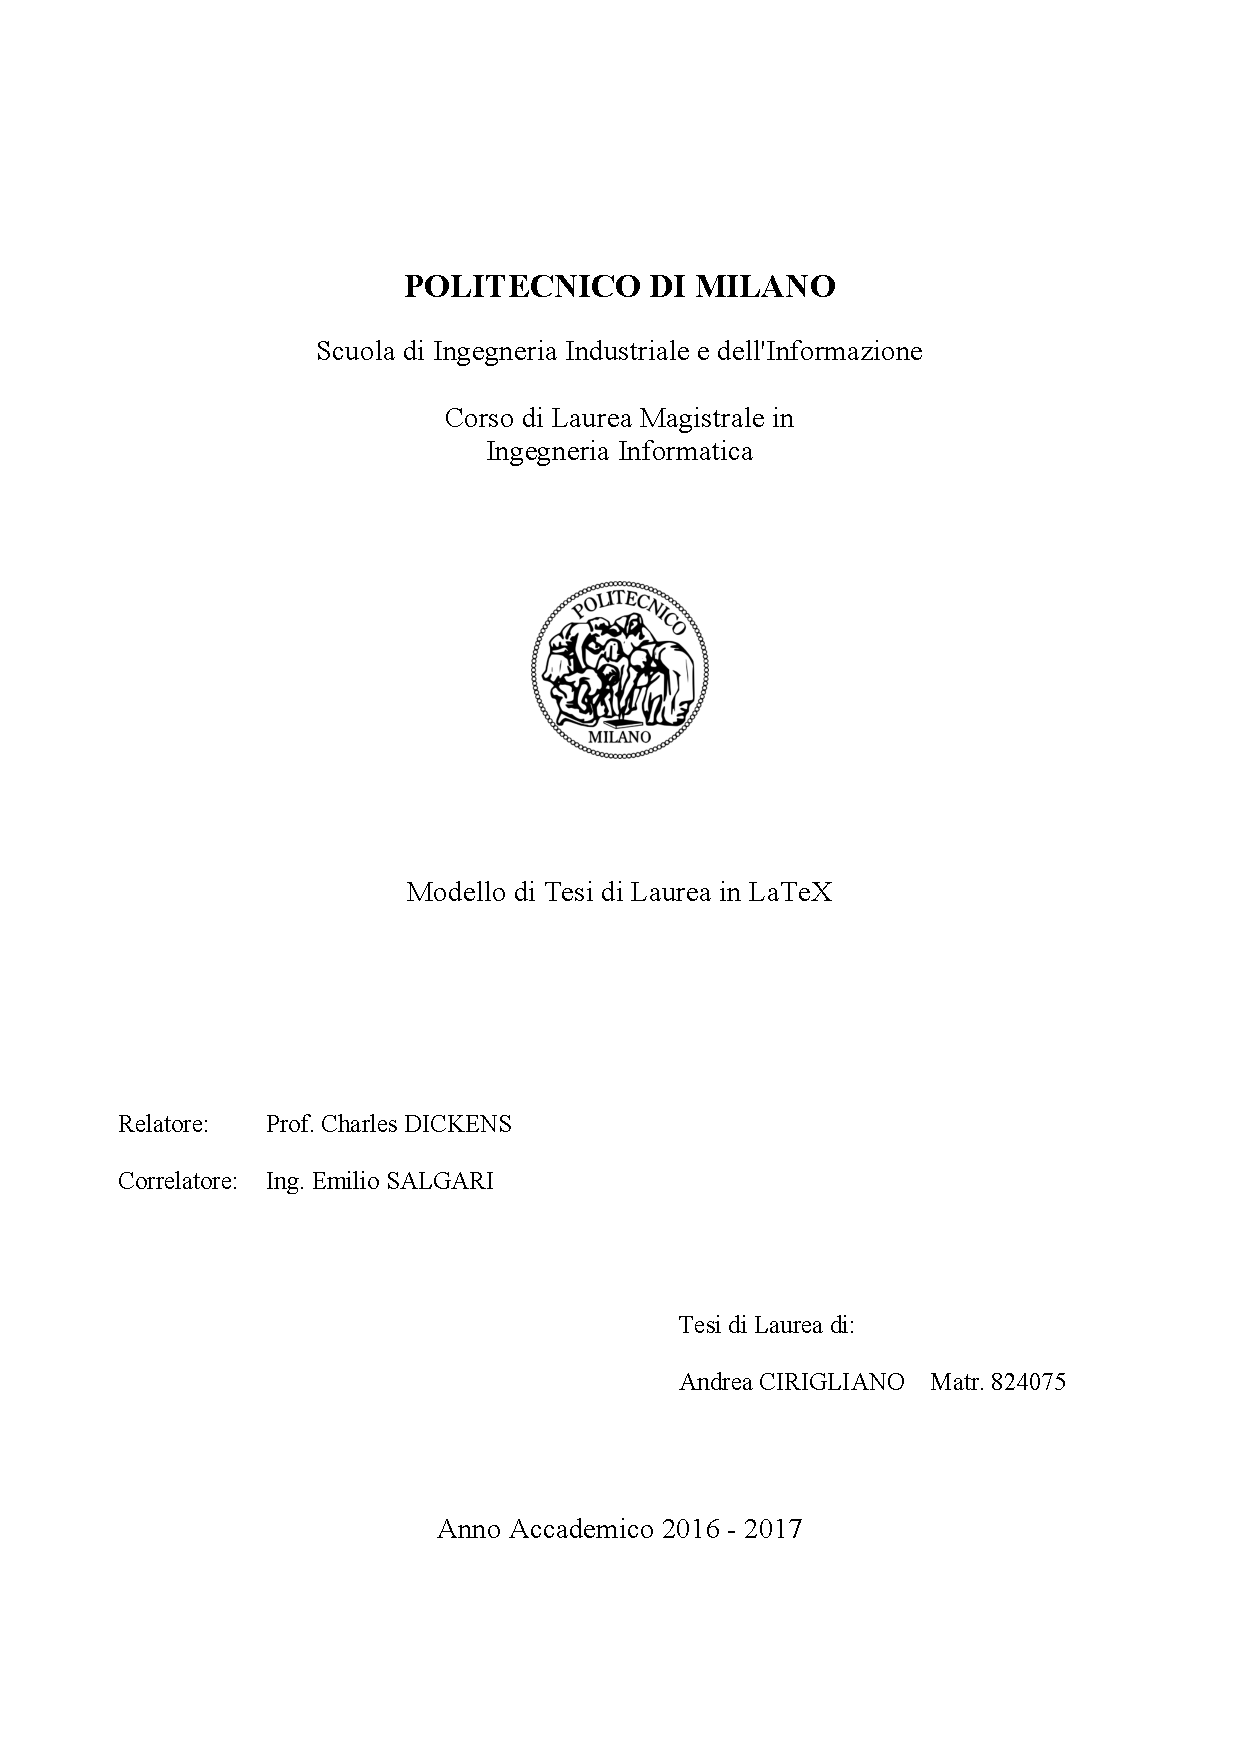
\includepdf{Frontespizio-Official-Word.pdf}
% %
% % ------------------------------------------------------------------------ %
% !TEX encoding = UTF-8 Unicode
% !TEX TS-program = pdflatex
% !TEX root = ../Tesi.tex
% !TEX spellcheck = it-IT
% ------------------------------------------------------------------------ %
%
% ------------------------------------------------------------------------ %
% 	COLOPHON
% ------------------------------------------------------------------------ %
%
\clearpage
%
\phantomsection
%
\thispagestyle{empty}
%
\pdfbookmark[1]{Colophon}{Colophon}
%
% ------------------------------------------------------------------------ %
%
\hfill
%
\vfill
%
% ------------------------------------------------------------------------ %
%
\noindent\myName:
%
\textit{\myTitle} \textbar\
%
\myThesis\ in \myDegree, \myUni.
%
\\
%
\textcopyright\ Copyright \myTime.

\vspace{0.5cm}
\hrule
\bigskip

\noindent{\myUni}: \\
\href{http://\myUrlUni}{\myUrlUni}

\medskip
\noindent{\myFaculty}: \\
\href{http://\myUrlFaculty}{\myUrlFaculty}
%
% ------------------------------------------------------------------------ %
% %
% ------------------------------------------------------------------------ %
% !TEX encoding = UTF-8 Unicode
% !TEX TS-program = pdflatex
% !TEX root = ../Tesi.tex
% !TEX spellcheck = it-IT
% ------------------------------------------------------------------------ %
%
% ------------------------------------------------------------------------ %
% 	RINGRAZIAMENTI
% ------------------------------------------------------------------------ %
%
\cleardoublepage
%
\phantomsection
%
\pdfbookmark{Acknowledgments}{Acknowledgments}
%
\chapter*{Acknowledgments\\\textit{Ringraziamenti}}
%

\textit{
Ringrazio Marco, che mi ha dato la possibilità di vivere e lavorare in un luogo unico come il NECSTLab, e che con la sua energia ha saputo spronarmi e migliorarmi.}

\medskip
\textit{
Ringrazio Alessandro, che ha saputo dirigermi e correggermi, e che mi ha lasciato larga autonomia nel mio percorso.
}

\medskip
\textit{
Ringrazio tutti i ragazzi che ho incontrato in NECSTLab, che non hanno mai esitato ad aiutarmi o divertirmi durante il lavoro.
}

\medskip
\textit{
E da ultimo, ringrazio le persone che con l'affetto mi hanno dato la gioia e la serenità delle mie giornate: mia sorella Antonella, i piccoli Carola e Luca, i miei genitori, mamma Maria e papà Giuseppe e Elena, lei che ha saputo essere protagonista dei miei istanti.}
%

\bigskip

\hfill \textit{Andrea}


\hfill \textit{\myLocation, \myTime}

%
% ------------------------------------------------------------------------ %
% %
% ------------------------------------------------------------------------ %
% !TEX encoding = UTF-8 Unicode
% !TEX TS-program = pdflatex
% !TEX root = ../Tesi.tex
% !TEX spellcheck = it-IT
% ------------------------------------------------------------------------ %
%
% ------------------------------------------------------------------------ %
% 	DEDICA
% ------------------------------------------------------------------------ %
%
\cleardoublepage
%
\phantomsection
%
\thispagestyle{empty}
%
\pdfbookmark{Dedica}{Dedica}
%
\vspace*{\stretch{1}}
%
\begin{flushright}
\textit{a te,\\ovunque tu sia,\\e qualunque percorso di vita tu abbia intrapreso.}
\end{flushright}
%
\vspace{\stretch{2}}
%
% ------------------------------------------------------------------------ %
%
% ------------------------------------------------------------------------ %
% !TEX encoding = UTF-8 Unicode
% !TEX TS-program = pdflatex
% !TEX root = ../Tesi.tex
% !TEX spellcheck = it-IT
% ------------------------------------------------------------------------ %
%
% ------------------------------------------------------------------------ %
% 	INDICI
% ------------------------------------------------------------------------ %
%
\cleardoublepage
%
% ------------------------------------------------------------------------ %
%
% Indice Generale
%
\pdfbookmark{\contentsname}{tableofcontents}
%
\setcounter{tocdepth}{2}
%
\tableofcontents
%
\cleardoublepage
%
% ------------------------------------------------------------------------ %
%
% Indice delle Figure
%
\phantomsection
%
\pdfbookmark{\listfigurename}{lof}
%
\listoffigures
%
\cleardoublepage
%
% ------------------------------------------------------------------------ %
%
% Indice delle Tabelle
%
\phantomsection
%
\pdfbookmark{\listtablename}{lot}
%
\listoftables
%
\cleardoublepage
%
% ------------------------------------------------------------------------ %
%
% Indice dei Listati di Programma
%
% \phantomsection
% %
% \pdfbookmark{\lstlistlistingname}{lol}
% %
% \lstlistoflistings
% %
% %listings and algorithms in same page
% \begingroup
% \let\clearpage\relax
% \listofalgorithms
% \endgroup
% %
% \cleardoublepage
%
% ------------------------------------------------------------------------ %
%
% ------------------------------------------------------------------------ %
% !TEX encoding = UTF-8 Unicode
% !TEX TS-program = pdflatex
% !TEX root = ../Tesi.tex
% !TEX spellcheck = it-IT
% ------------------------------------------------------------------------ %
% ------------------------------------------------------------------------ %
% 	ABSTRACT
% ------------------------------------------------------------------------ %
%
\cleardoublepage
%
\phantomsection
\addcontentsline{toc}{chapter}{Abstract}
%
%\pdfbookmark{Abstract}{Abstract}
%
% ------------------------------------------------------------------------ %
% consento presenza di più capitoli nella stessa pagina
%\begingroup
%\let\clearpage\relax
%\let\cleardoublepage\relax
%\let\cleardoublepage\relax
% ------------------------------------------------------------------------ %
%
\chapter*{Abstract}
\markboth{Abstract}{Abstract}
%
During the past few years, a lot of effort has been put in the research area of connected sensors and actuators, the so-called \emph{Internet-of-Things}. A big portion of this research is applied to the domain of Smart Buildings, where connected devices are exploited to increase comfort, safety, and energy sustainability.
However, there can be identified some missing tiles that get more difficult the adoption of such technologies in real buildings.
The work done in this thesis tries to solve two of these missing tiles.

First, is analyzed the problem of knowing number and position of building occupants, and an \emph{Occupancy Monitoring} system is proposed. One of the main limitations of existing solutions is the inability to provide both long time monitoring (many hours of execution) and a non-intrusive approach from the occupant point of view.
With the proposed system, called BlueSentinel, we tried to exploit the Bluetooth Low Energy technology at low level to detect the presence of occupants inside the building. The approach allows the system to run continuously for many hours without heavily affect the mobile battery consumption.\\
The experimental results confirmed that the proposed approach is suitable to obtain a real-time occupancy information with a localization accuracy comparable to the state of the art.

The second part of this work tries to solve the problem of designing optimal Smart Building systems based on wireless devices. We tried to explain the challenges faced by designers during the installation of Smart Building systems that require the positioning of several hardware nodes, and the lack of automatic tools able to support this phase.\\
For these reasons, we propose an integrated CAD tool for both floor plan specification and node positioning, developed within an \mbox{open-source} CAD environment extensible through plug-ins. The tool is able to provide a near-optimal solution of node allocations, with the aim to reduce the installation costs. The results suggest that, depending on the available hardware types, total cost of the solution could be improved by the proposed model moving from homogeneous to mixed type allocation.

\medskip
%
\noindent \textbf{Keywords:} 
Smart Buildings; Occupancy Detection; Occupancy Monitoring; Indoor Localization; Indoor WSNs; Indoor WSNs Deployment;
%
\clearpage
%\vfill
%
% ------------------------------------------------------------------------ %
%
%
\cleardoublepage
%
\phantomsection
% \pdfbookmark{Abstract}{Abstract}
% %
% \markboth{Abstract}{Abstract}
%
\chapter*{Abstract}
%
Negli ultimi anni, il continuo avanzamento tecnologico nel campo delle reti di sensori e attuatori ha generato il fenomeno del cosiddetto \emph{Internet-of-Things}. Larga parte della ricerca in questo campo è rivolta alla realizzazione di \emph{edifici intelligenti} (Smart Buildings), in cui numerosi dispositivi connessi sono utilizzati per aumentare il comfort, la sicurezza ed il risparmio energetico degli edifici. Tuttavia, esistono ancora alcuni problemi irrisolti che ostacolano la diffusione di queste tecnologie negli edifici odierni. Il lavoro descritto in questa tesi tenta di risolvere due di questi problemi.

Per prima cosa viene affrontato il problema di rilevare in tempo reale il numero e la posizione degli utenti all'interno di un edificio. I sistemi esistenti in letteratura non raggiungono lunghi tempi di esecuzione, o utilizzano approcci invasivi per gli abitanti dell'ambiente.
A tal proposito verrà presentato BlueSentinel, il sistema di \emph{Occupancy Monitoring} realizzato sfruttando il protocollo Bluetooth Low Energy per monitorare a lungo la posizione degli utenti, senza gravare sul consumo di batteria mobile.\\
Le analisi sperimentali confermano che l'approccio proposto è adatto a rilevare in tempo reale la posizione degli utenti, con un'accuratezza della localizzazione in linea con i metodi proposti nello stato dell'arte.

Successivamente, viene affrontato il problema del design di sistemi per Smart Buildings basati su nodi wireless. Durante l'installazione di questi sistemi, ad esempio di localizzazione o monitoraggio, il posizionamento dei nodi è critico, influendo sul costo e le performance del sistema. Tuttavia, questo processo viene ancora realizzato manualmente a causa della mancanza di tool automatizzati.\\
Proponiamo dunque una applicazione CAD per la specifica della struttura di un edificio e l'allocazione ottimale di nodi sensori. L'applicazione, rilasciata in maniera open-source ed estendibile tramite plugins, è in grado di posizionare i nodi in modo da massimizzare l'accuratezza del sistema, e allo stesso tempo fornire soluzioni a basso costo.
I risultati mostrano che il tool proposto è in grado di fornire, a parità di accuratezza, soluzioni meno costose allocando nodi eterogenei.

\medskip
%
\noindent \textbf{Parole chiave:} 
Edifici Smart; Rilevamento dell'Occupazione; Monitoraggio dell'Occupazione; Localizzazione Indoor; Indoor WSNs; Posizionamento Automatico di WSNs Indoor;
%
% ------------------------------------------------------------------------ %



%
% ------------------------------------------------------------------------ %
% !TEX encoding = UTF-8 Unicode
% !TEX TS-program = pdflatex
% !TEX root = ../Tesi.tex
% !TEX spellcheck = it-IT
% ------------------------------------------------------------------------ %
% ------------------------------------------------------------------------ %
% 	SOMMARIO
% ------------------------------------------------------------------------ %
%
\cleardoublepage
%
\phantomsection
\addcontentsline{toc}{chapter}{Sommario}


\markboth{Sommario}{Sommario}
%
\chapter*{Sommario}
Oggigiorno, l'avvento tecnologico delle reti di sensori e attuatori ha permesso di modernizzare gli edifici per migliorarne il monitoraggio e l'automazione. In particolare, l'uso della tecnologia è rivolto ad incrementare il comfort degli utenti, la sicurezza e l'efficienza energetica degli ambienti interni.\\
Gli edifici intelligenti (o \emph{Smart Buildings}) stanno diventando una realtà con l'adozione di sistemi automatici detti Building Management Systems (BMS), vale a dire sistemi di controllo che integrano l'infrastruttura di monitoraggio e attuazione sottostante con un motore di decisione logica ad alto livello. Queste decisioni sono solitamente basate su impostazioni dell'amministratore e regole definite dall'utente, oltre che da algoritmi di apprendimento automatico più complessi.

In questo contesto, identificare in tempo reale il numero degli occupanti nell'edificio, la loro posizione e l'identità di ciascuno può essere essenziale per fornire la logica di attuazione dell'edificio. Per citare un esempio, i sistemi di condizionamento, riscaldamento, e ventilazione dell'aria (sistemi HVAC) possono essere modulati in base al numero degli occupanti, aumentando il comfort termico, ed evitando sprechi di energia. Il problema di rilevare in tempo reale la posizione degli utenti in un edificio, noto come il problema dell'\emph{Occupancy Detection}, è uno dei due obiettivi principali di questa tesi.

La sostenibilità energetica non è l'unico scopo dell'occupancy detection. Recentemente, sistemi di sicurezza avanzati sono stati studiati e adottati negli edifici commerciali per rispondere a situazioni di pericolo e limitare i danni e le vittime. Il compito principale di questi sistemi è quello di rilevare eventi di crisi e fornire una risposta adeguata. La capacità di rilevare la posizione degli utenti all'interno dell'edificio può essere cruciale per assistere evacuazioni o recuperi di salvataggio.

Il problema di localizzare gli utenti in ambienti interni è intrinsecamente difficile, sia tecnologicamente che per quanto riguarda l'interazione con l'utente. Per applicazioni ad uso esterno, l'uso del GPS si è rivelata la migliore soluzione in termini di costo, precisione e facilità d'uso, aumentandone la diffusione. Per le applicazioni in ambienti interni, la mancanza di sistemi di localizzazione in edifici moderni è causato dall'inesistenza di una soluzione tecnologica a basso costo, con sufficiente precisione e buona usabilità. Inoltre, il problema specifico di rilevamento dell'occupazione pone ulteriori sfide rispetto ai sistemi di posizionamento indoor (IPS) generici. La differenza fondamentale tra i sistemi di occupancy monitoring e i IPS tradizionali risiede nel tempo di esecuzione. L'occupancy monitoring richiede di monitorare gli utenti per molte ore del giorno, mentre l'utilizzo di un IPS è in genere limitato all'orientamento e alla navigazione dell'utente.
Un lungo tempo di esecuzione porta innanzitutto ad un enorme problema di consumo della batteria per soluzioni che prevedono dispositivi mobili nel processo di localizzazione. Le applicazioni di localizzazione consumano in genere molta energia, e mentre ciò può essere accettato per un uso limitato, diventa impraticabile per molte ore di esecuzione.\\
Un altro problema che deriva dal lungo monitoraggio è l'invadenza del sistema sull'attività degli occupanti. Sistemi di occupancy monitoring basati su immagini provenienti dalle telecamere possono sollevare problemi di privacy, anche in spazi di lavoro condivisi come uffici e sale riunioni.

Un altro requisito impegnativo di molti sistemi di rilevamento dell' occupazione, fra cui quello proposto in questa tesi, è di fornire le informazioni di occupazione in tempo reale. Per essere considerati in tempo reale, i dati di posizione dovrebbero essere ricevuti dal sistema di back-end con un ritardo massimo di 2-3 secondi; in caso contrario l'automazione non viene percepita come utile o reattiva dall'utente. Ciò significa che le caratteristiche ambientali come temperatura, umidità, luce e CO2 che sono legate all'occupazione, non possono essere facilmente sfruttate per il rilevamento in tempo reale a causa del loro tempo di risposta lento.

Il sistema di occupancy monitoring proposto, chiamato BlueSentinel, è stato realizzato per monitorare a lungo la posizione degli utenti senza gravare sul consumo di batteria mobile. BlueSentinel è stato realizzato sfruttando il protocollo Bluetooth Low Energy a basso livello, per soddisfare i requisiti di real-time e bassa invadenza sugli utenti. Il sistema è composto, oltre che da una applicazione per smartphone, da una rete di nodi sensore posizionati nell'edificio in grado di rilevare la presenza degli utenti. I segnali percepiti vengono raccolti in maniera centralizzata da un server, dove la posizione di ogni persona viene calcolata con un algoritmo di classificazione.

\medskip
Per risolvere il problema dell'occupancy detection, così come altri sistemi per Smart Buildings (ad esempio gestione delle emergenze o del comfort termico), è comune impiegare numerosi dispositivi connessi con funzionalità di sensoristica, attuazione o di comunicazione wireless. 
L'elevato livello di eterogeneità e la mancanza di standardizzazione tra le tecnologie rende il design di questi ambienti un compito molto impegnativo, perché ogni installazione deve essere progettata ed eseguita manualmente, in maniera ad-hoc per la specifica applicazione. D'altra parte, molti sistemi diversi mostrano caratteristiche comuni, come la stretta dipendenza con la pianta dell'edificio, condividendo anche requisiti simili come un'allocazione dei nodi che fornisce connettività wireless e copertura all'ambiente.

La posizione di ogni nodo influenza fortemente le prestazioni del sistema, in quanto una cattiva allocazione può portare a zone non monitorate. Il numero di nodi impiegati, oltre a influire sul costo di installazione, grava anche sul consumo energetico complessivo del sistema, un parametro particolarmente critico da considerare soprattutto per sistemi di risparmio energetico.
La scelta dei nodi hardware può diventare ancor più difficile per la disponibilità sul mercato di diversi dispositivi e componenti che si differenziano per il costo, il consumo di potenza e la portata dei segnali wireless.

Nonostante l'importanza del posizionamento dei nodi, molti sistemi per Smart Buildings proposti in letteratura ignorano il problema per tutti gli ambienti che differiscono da quello di test originale.
Senza un approccio sistematico, lo spazio di progettazione non viene esplorato in maniera efficace, portando a soluzioni non ottimali. In tale contesto, lo sviluppo di strumenti in grado di automatizzare parte del flusso di progettazione dei sistemi per Smart Buildings è essenziale.

La mancanza di strumenti automatici di supporto di questo tipo ci ha indotto a sviluppare un'applicazione CAD specifica allo scopo.
Il lavoro che costituisce la seconda parte di questa tesi consiste in una applicazione CAD per la progettazione di sistemi per Smart Buildings basati sull'installazione di nodi hardware nell'ambiente interno. Lo strumento fornisce un algoritmo per la distribuzione efficiente di sistemi di localizzazione wireless, con l'obiettivo di massimizzare l'accuratezza della localizzazione mantenendo i costi di installazione contenuti.
Il progetto, rilasciato in maniera open-source, è estendibile tramite plugin in modo da poter modellizzare sistemi per Smart Buildings con diverse caratteristiche e requisiti.




%
\cleardoublepage
%
% ------------------------------------------------------------------------ %
% 	MAINMATTER
% ------------------------------------------------------------------------ %
%
\mainmatter
%
% ------------------------------------------------------------------------ %
% !TEX encoding = UTF-8 Unicode
% !TEX TS-program = pdflatex
% !TEX root = ../Tesi.tex
% !TEX spellcheck = it-IT
% ------------------------------------------------------------------------ %
%
% ------------------------------------------------------------------------ %
% 	INTRODUZIONE
% ------------------------------------------------------------------------ %
%
\cleardoublepage
%
\phantomsection
%
\addcontentsline{toc}{chapter}{Introduction}
%
\chapter*{Introduction}
%remove * to count from 1
%
\markboth{Introduction}{Introduction}	% headings
%
\label{cap:intro}
%
% ------------------------------------------------------------------------ %
%
On average, people spend approximately 70\% of their time indoors \cite{Roulet2001}, such as in offices, schools, and at home.
In the last years, the advent of sensors networks have enabled buildings to be retrofit for improved monitoring and automation.
In particular, the use of technology is intended to increment the occupants comfort, their safety and the energy efficiency of the indoor environments.
Smart Buildings are becoming a reality with the adoption of Building Management Systems (BMS), i.e. control systems that integrate the underlying monitoring infrastructure with a logic decision engine. These decisions are usually based on administrator policies or user-defined rules, other than more complex machine learning algorithms.
In this context, identifying in real-time the number of occupants in the building, their location and even the identity of each one can be essential to provide the building behavior logic. For instance, Heating, Ventilation and Air Conditioning (HVAC) systems can be modulated according to the number of occupants, increasing thermal comfort while avoiding energy wastes.
The problem of knowing in every instant the location of users in a building, known as the \emph{Occupancy Detection} problem, is one of the two main targets of this work.
% Occupancy detection, that at first glance could appear equal to the more conventional indoor localization, is characterized by different requirements, making the implementation and the adoption of such systems even more challenging.
% Accennare bluetooth low energy?

In order to solve the occupancy detection problem, as well as other smart building systems like thermal comfort or emergency management, it's common to employ several connected devices with sensor, actuator or network capabilities. During the testing phase of our system, but also trying to verify existing approaches from the state of the art, we experienced the difficulty of tedious, error-prone and time consuming tasks like the correct allocation of devices in the environment. During the installation of such systems, the choice of the nodes type and quantity, the proper placement of each one heavily affect the accuracy and the cost of the system. The lack of supporting tools for the design of indoor monitoring systems induced us to develop a CAD based application tailored for the purpose. The development of the mentioned application comprises the second main part of this thesis.




%
\section{Motivations}
Energy sustainability is one of the key target of smart (or green) buildings.
From 1980 to 2010, energy in the United States has increased 53\% \cite{doe}. In 2010, heating, ventilation, and air-conditioning (HVAC) consumed 42\% of the energy used in the United States.

There are two different parts of HVAC systems usage that should be affected by occupancy; temperature and ventilation.
Temperature control is dependent on whether a space is occupied. However, indoor environments are often conditioned assuming a constant occupancy. This leads to heating or cooling empty rooms. One method of reducing consumption is to condition based on the actual binary state of occupancy.
Ventilation instead, used to control CO2 levels and air pollutants, depends on the number of people occupying a space. Also in this case, spaces that are only partially occupied could be over-ventilated, leading to loss of conditioned air and thus thermal energy. For this purpose, standards have been issued to recommend ventilation for acceptable indoor air quality depending on occupation (ASHRAE standard 62.1 \cite{ashrae}).
The usage of energy-hungry appliances like HVAC systems can be improved not only by the real-time occupancy information, but also from occupancy probability profiles built on top of historical data. For instance, the information that in a certain office, every Friday the last employee leaves the room at 5 p.m. with a probability of 90\% can be exploited to reduce energy consumption.

\smallskip
Another purpose of smart buildings is safety. Automated systems that respond to harmful situations limiting damages and victims have been studied and adopted in commercial and private buildings since many decades. The primary job of these systems is to detect crisis events and provide a suitable response. The ability to detect the position of users inside the building can be crucial to assist evacuations or rescue operations. For example, the safety system could trigger alarm notifications tailored on user's position; escape routes and emergency exits might be highlighted with labels and lighting panels.

\smallskip
Occupancy detection can be exploited to build indoor location data analytics, that measure time spent by visitors in particular locations and which routes were used. This enables shopping stores find out how many people pass a certain zone during the day or which hours of the week are the least busy. Location monitoring allows shopping malls to provide rewards, discounts and targeted advertisement to their customers. At the same way in which web analytics are used by web managers to optimize their pages, indoor location data analytics can be exploited by store owners to increase profitability of their business.

\section{Challenges}
The problem of locate users in indoor environments is intrinsically hard, in both the technological and the user interaction sides. For outdoor applications the use of GPS has revealed to be the best solution in terms of cost, accuracy and ease of use, leading to its widespread popularity. For indoor applications, the lack of localization systems in modern buildings is caused exactly by the nonexistence of a low-cost technological solution with sufficient accuracy and good usability. In addition, the specific occupancy detection problem poses additional challenges to the generic Indoor Positioning Systems (IPS). The distinction between occupancy monitoring systems and traditional IPSs will be explained in detail in section \ref{subsec:wips_od}, but intuitively the key difference relies in the execution time. Occupancy monitoring requires to monitor the users for many hours of the day, while the execution of an IPS is typically limited to the orientation or navigation task of the user. 

\smallskip
First of all, long execution time leads to a huge \textbf{battery consumption} problem for solutions that involve mobile devices in the localization process. Localization applications are typically very battery hungry, and whereas this can be accepted for short usage, it becomes unfeasible for many hours of execution.

\smallskip
Another issue derived from the long monitoring is the \textbf{intrusiveness} on the occupants activity. Occupancy detection systems based on images coming from cameras can raise privacy issue, even in working spaces like offices or meeting rooms.
Solutions that relies on the assumption that the occupants are always accompanied by a tag, a smartphone or a wearable device are also intrusive in the sense that a certain level of effort is required to the user. This level of effort can be perceived differently depending on the situations. At work, where the user is used to guarantee phone call and email availability, the effort can be nearly zero; at home instead, where some users are used to empty their pockets as soon as they are inside, the effort can be high.
Again, battery consumption affect also the system intrusiveness.
%Smart devices are becoming omnipresent around people and they can be considered as an extension of our-selves.
%The only actual weak point of every smart device is the battery life, and thus it became an issue also for the user daily activity.
%For this reasons, occupancy detection systems that rely on smart devices should carefully consider the energy efficiency of the device.
A system that cause a considerable increase in battery drain directly afflict the user comfort and peace of mind, and can bring the user to leave the application.

\smallskip
A challenging requirement of some occupancy detection systems, including the proposed one, is to provide the occupancy information in \textbf{real-time}. In order to be considered real-time, the location data should be received from the system back-end with a maximum delay of 2-3 seconds, otherwise the automation will not be perceived as useful or responsive. This means that ambient characteristics like temperature, humidity, light, CO2 and so on, that are related to occupancy, can't be easily exploited for real-time detection due to their slow time response. 

\smallskip
Other issues that discourage that adoption of occupancy monitoring systems are in common with traditional IPSs. When the system is composed by transmitting nodes or sensor networks, the \textbf{cost} of the hardware purchase and the \textbf{installation} of appliances can be onerous. Even for small buildings, the choice of the nodes quantity and a correct placement able to guarantee space coverage can be cumbersome. Adjust and move devices to tune the system performances is time-consuming and sometimes unfeasible. To address this specific problem, we developed a CAD application for the design of smart building systems based on the installation of hardware nodes across the indoor space. The tool, that provide cost-effective deployment of wireless localization systems, will be described in chapter \ref{cap:cad}.

\section{Scope and Contributions}
This thesis is about occupancy detection and monitoring in smart buildings.
The work done in this thesis can be summarized in two main parts.

\medskip
First, an occupancy monitoring system based on Bluetooth Low Energy (BLE) is proposed. the key aspects of the proposed system are:
\begin{enumerate*}[label={\textbf{(\arabic*)}}]
\item extremely low battery consumption allows the system run continuously for many hours;
\item real-time occupancy detection;
\item non-intrusive system from the user point of view;
\item simplified installation and training.
\end{enumerate*}

\medskip
The second part of this thesis is about design automation for smart building systems based on sensor and network devices. The rationale of the developed application comes from a real-world necessity that we experienced during the arrangement of wireless indoor localization systems. The key contributions of the proposed application with respect to other existing approaches are:
\begin{enumerate*}[label={\textbf{(\arabic*)}}]
\item a CAD interface to specify building floor-plan and functional components of the smart environment;
\item an algorithm for hardware nodes allocation that provides to designers a cost-effective placement of devices;
\item a site-specific model for wireless indoor localization accuracy optimization that keeps into account the actual structure of the building;
\item The integration of the tool within an \mbox{open-source} application framework able to extend the system by means of JavaScript or C++ plug-ins.
\end{enumerate*}

%\clearpage

\section{Document Organization}
%
\par The thesis is structured as follows:
%
% ------------------------------------------------------------------------ %
%
\begin{description}
%
\item[{\hyperref[cap:soa]{The first chapter}}] explains and investigates the occupancy monitoring problem for smart buildings. The state of the art is analyzed reporting the most relevant existing approaches grouped by their respective enabling technologies. A particular attention is directed to wireless-based indoor positioning systems, how they have been exploited for occupancy monitoring and their limitations in this specific context. In this part are also reported some concepts of WiFi and Bluetooth Low Energy protocols useful to understand the limitations of existing approaches and the design choices of the adopted solution.
%
\item[{\hyperref[cap:bluesentinel]{The second chapter}}] describes the proposed BLE occupancy monitoring system. First, the feasibility study is reported, explaining also the reasons of the adopted design and the technology employed. Then will be illustrated the architecture of the system, passing through application, sensing and back-end layers. On the application side, will be discussed the potentiality and limitations of the BLE signal advertisement of recent smartphones, one of the key functionalities exploited in our system. Then, at sensors level, will be reported the different methods of synchronization and signal filtering experimented. For the back-end side, are reported the different classification methods employed for users localization, and their performances with respect to the ground truth. Here will be also illustrated how the occupancy information has being visualized in a web application.
%
\item[{\hyperref[cap:cad]{The third chapter}}] shows the design challenges of smart building systems based on the installation of several hardware nodes such as sensors or wireless access points. To address this problem, the developed supporting tool is presented. The application, based on a CAD interface for floor-plans specification, implements an heuristic algorithm for an optimal deployment of nodes. Although the heterogeneity and lack of standardization, is explained how we tried to provide a general-purpose tool, offering three different indoor localization techniques and the ability to extend the application with third-party plug-ins.
%
\item[{\hyperref[cap:results]{In the fourth chapter}}] will be described our system deployment in a real environment and the experimental results obtained. \lipsum[2]
%
\end{description}
%
% ------------------------------------------------------------------------ %
%
% ------------------------------------------------------------------------ %
% !TEX encoding = UTF-8 Unicode
% !TEX TS-program = pdflatex
% !TEX root = ../Tesi.tex
% !TEX spellcheck = it-IT
% ------------------------------------------------------------------------ %
%
% ------------------------------------------------------------------------ %
% 	STATO DELL'ARTE
% ------------------------------------------------------------------------ %
%
\chapter[Occupancy Monitoring and State of the Art]{Occupancy Monitoring Basics and State of the Art}
%
%\markboth{x}{y}	% headings
%
\label{cap:soa}
%
%cosa sono gli smart buildings e perchè è importante l'occupancy monitoiring

Smart buildings are environments like offices or schools able to exploit sensors, devices and appliances to observe users activity and adapt autonomously taking decisions to achieve comfort, safety and energy efficiency. Considering the fast development of technologies for connected sensor and actuator (the so called \emph{Internet of Things}), since few years smart buildings are becoming a reality from a technological point of view.

Both the industry and the academia have put a lot of effort in the research of smart buildings. In some commercial products the term \emph{smart} is often referred to devices that can be remotely accessed and managed, even though there is no intelligence involved. In this thesis, the term \emph{smart building} refers to the concept of environment able to cooperate and self-organize its components observing the indoor space.

\medskip
One of the main components of a smart building is the \textbf{Occupancy Monitoring system}, i.e. a system able to detect the number (or even the identity) of the occupants in every room or zone of the building. Occupants play a key role in the objectives of smart buildings. User comfort can be improved controlling automatically the environment temperature, humidity and brightness, setting all the parameters exploiting user defined preferences. In this scenario, user identification and localization inside the building is fundamental. 

\smallskip
In order to guarantee the building safety, the knowledge of the occupants position in real-time can be precious. In case of emergencies like fires, escape routes and emergency exits might be highlighted with notifications targeted to the specific user's location \cite{Piscitello2015}. Rescue operations can be organized faster and more efficiently when the position of injured occupants is known. Complex safety systems are even able to automatically detect dangerous situations like terrorist attacks when fast mass-movement of people happen from a room to another.

\smallskip
Probably, the main purpose of smart buildings, also called green buildings in this case, is energy sustainability.
In the last few years, plenty of methods have been proposed to learn the building occupants habits and to use such information to forecast the energy consumption.
Many of these approach are based on the concept of \emph{Smart Grid}. Smart Grid is a traditional electric grid enhanced with a two-way communication between the provider and its customers to respond digitally and more efficiently at quickly changing electric demand.
The mentioned methods for smart buildings are able to select the most appropriate appliance usage scheduling given an energy reduction request coming from the smart grid. Also in this case an occupancy monitoring system is essential to recognize users activities.

\medskip
The expected outcome of an occupancy monitoring system is the detection in real-time (or with a tolerable delay) of every user inside the building, with their position. Usually, the occupant needs to be localized in a zone or room of the building, since this information is sufficient to automatize HVAC and lighting systems. In cases of automation based on user-defined preferences also the identification of each user is required by the system.
At first look, the occupancy monitoring problem can be associated to the more traditional problem of the indoor localization. Even though the two problem share some characteristics, we will see that conventional solution for indoor localization are not directly applicable for monitoring (section \ref{subsec:wips_od}).

\smallskip
In this chapter, we will see that a lot of effort has been put both from the industry and the academia in terms of research and product industrialization. However, some intrinsically hard challenges of the occupancy monitoring problem bring to the lack of an accessible solution with broad adoption.

%il problema sembra simile o identico al più tradizionale indoor localization. non è così perchè ....
%come vedremo i due problemi sono simili ma le classiche soluzioni di WIPS non sono direttamente applicabili per O.M.

% ------------------------------------------------------------------------ %
\section{Evaluation Metrics}
\label{sec:occupancy-metrics}
% The traditional concept of indoor localization is a service able to assist the user during orientation in an unknown space, and to assist the navigation from one point to another. in this scenario, the end-user is the main subject who benefits from the positioning information.\\
% With the diffusion of smart spaces that cleverly support their inhabitants, positioning information is becoming essential also on the infrastructure side, usually called Building Management System (BMS).

Occupancy Monitoring systems have the purpose to detect the number of occupants in a building, their position and in some cases also the identity of each one.
Occupancy detection solutions can range to deeply different implementations, depending on the technologies exploited to detect human presence. In this section will be defined some metrics and aspects of occupancy monitoring systems useful to evaluate and compare different solutions.

\medskip
A feature that characterizes different occupancy monitoring systems is \textbf{Resolution} (Fig~\ref{fig:resolution}): it represents the granularity of the measurement.

\begin{figure}
     \centering
     \subfloat[]{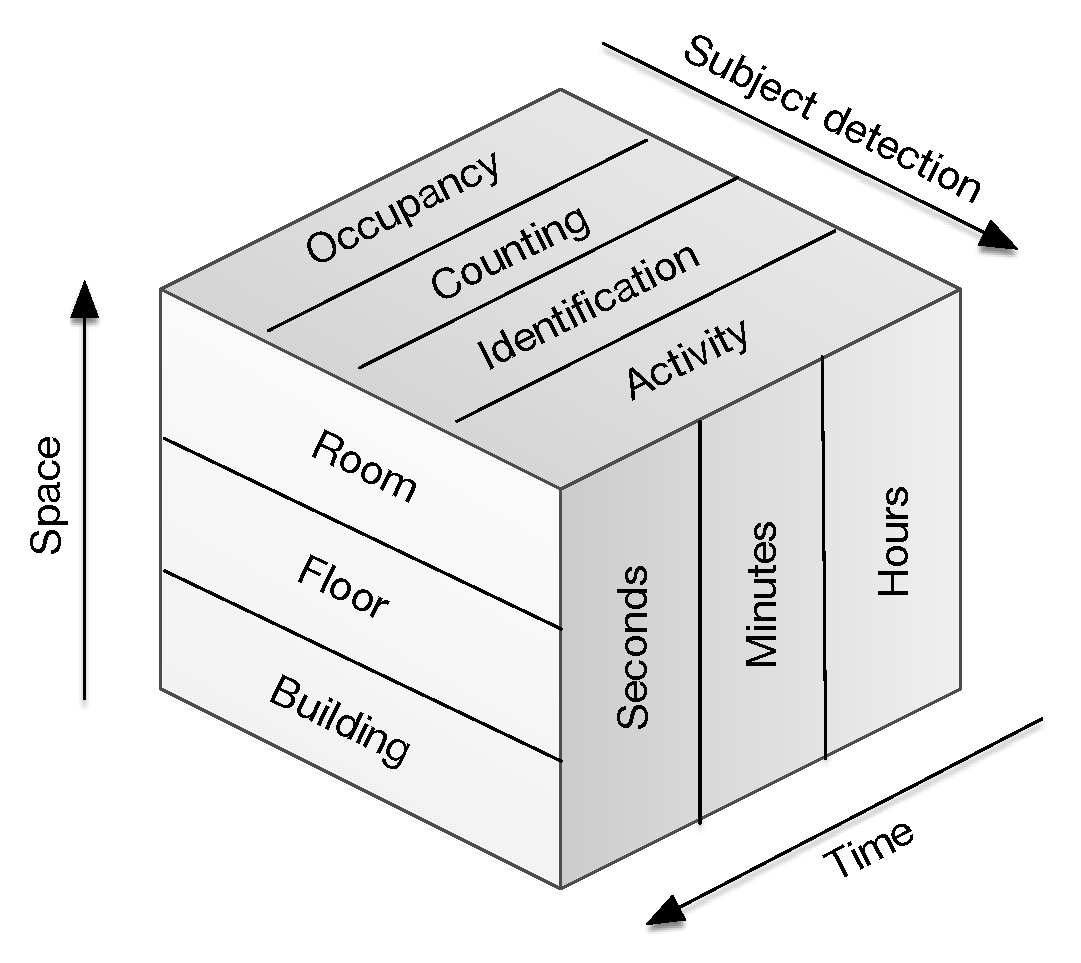
\includegraphics[width=0.5\linewidth]{resolution.pdf}\label{fig:resolution}}
     \subfloat[]{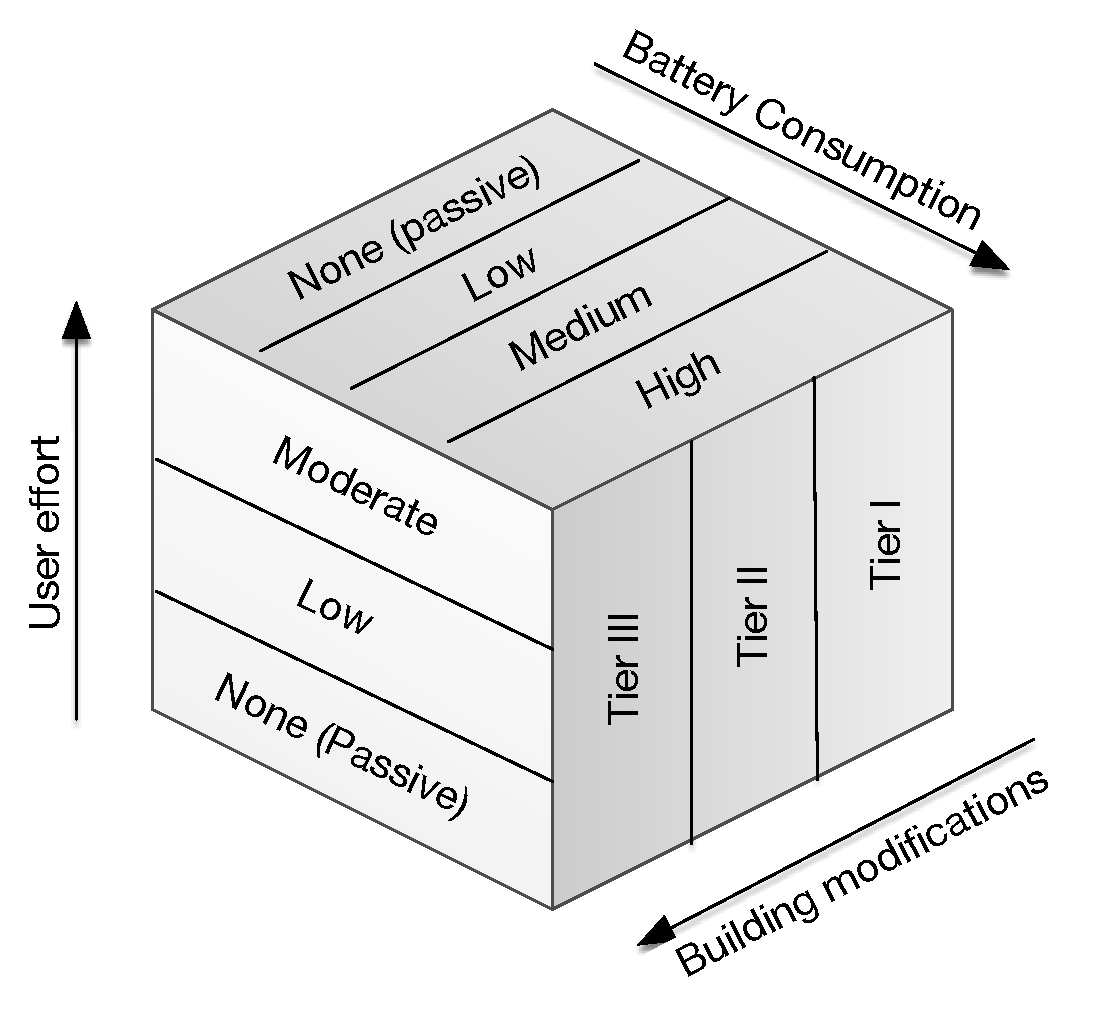
\includegraphics[width=0.5\linewidth]{intrusiveness.pdf}\label{fig:intrusiveness}}
     \caption[Occupancy Monitoring systems Resolution and Intrusiveness.]{\protect\subref{fig:resolution} Occupancy Monitoring systems Resolution. \protect\subref{fig:intrusiveness} Occupancy Monitoring systems Intrusiveness.}
	\label{fig:res_intr}
\end{figure}

% \begin{figure}
% \centering
% \subfloat[]{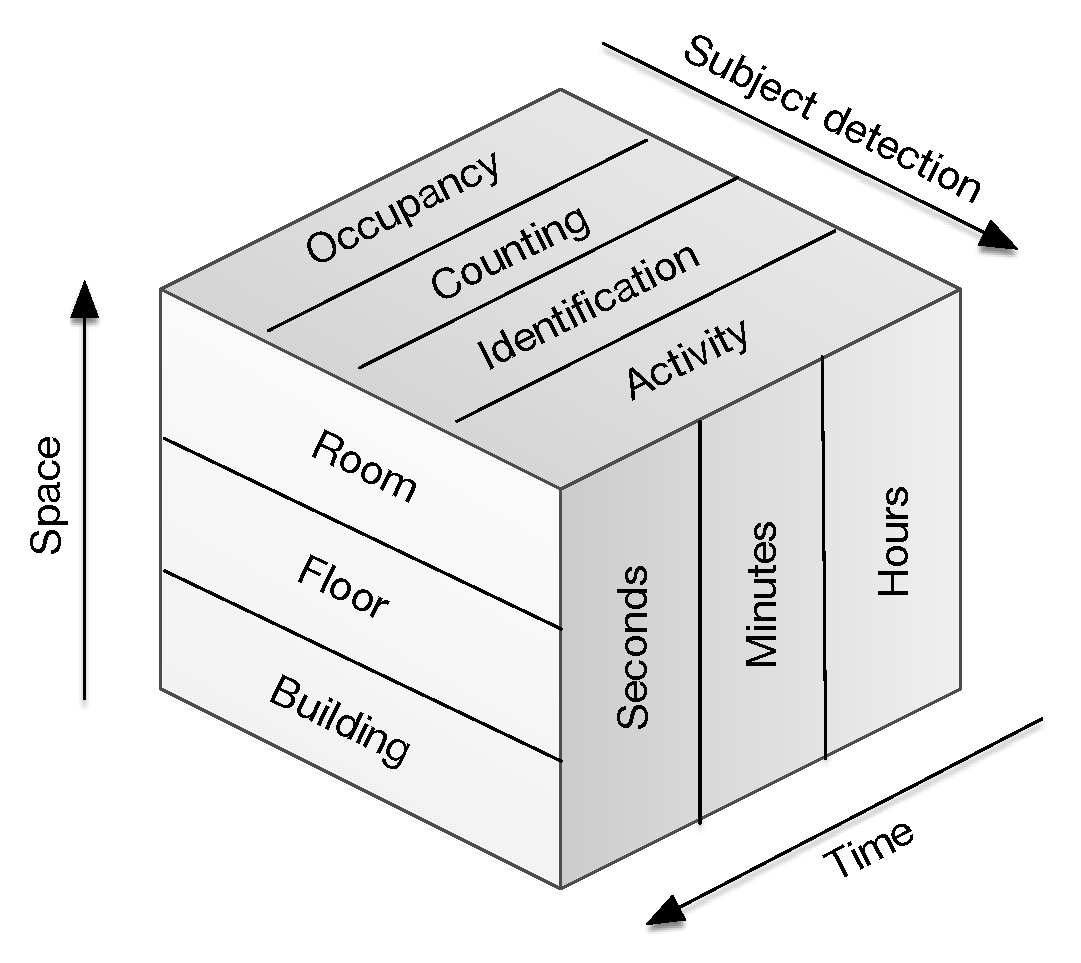
\includegraphics[width=0.5\linewidth]{resolution.pdf}\label{fig:resolution}}
% %
% \subfloat[]{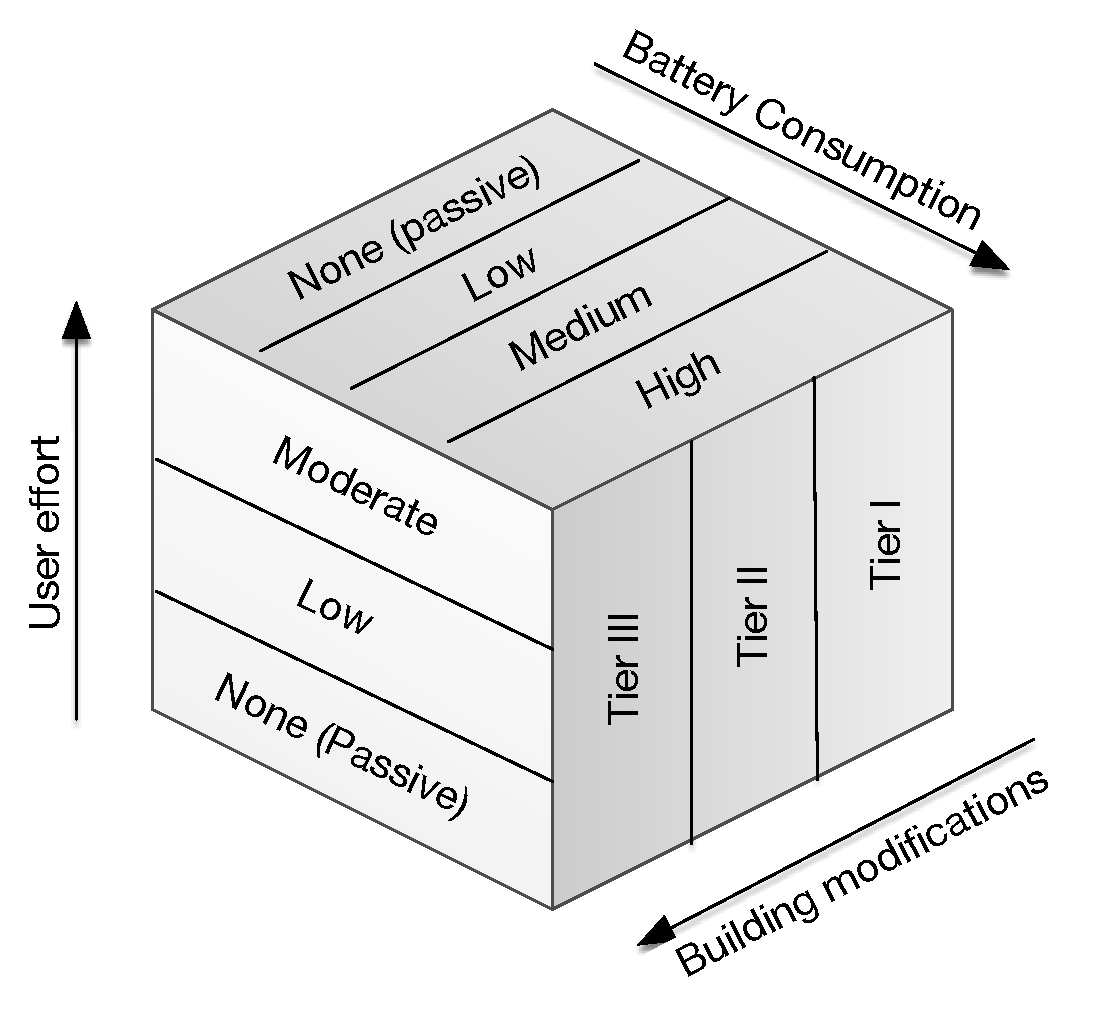
\includegraphics[width=0.5\linewidth]{intrusiveness.pdf}\label{fig:intrusiveness}}
% \caption[Occupancy Monitoring systems Resolution and Intrusiveness.]{\protect\subref{fig:resolution} Occupancy Monitoring systems Resolution. \protect\subref{fig:intrusiveness} Occupancy Monitoring systems Intrusiveness.}
% \label{fig:res_intr}
% \end{figure}

Resolution can refer to:
\begin{itemize}
\item Subject of the detection: from low to high resolution, the system can perceive only the occupied/unoccupied status of a zone, the number of people or even the identity of each person.
\item Space resolution, i.e. the smallest region in which the user can be localized. Can range from building zones to single rooms, desktop stations or cubicles.
%In this terms, occupancy monitoring usually requires lower levels of resolution than localization.
\item Temporal resolution indicates the smallest time span in which occupancy status transitions can be reported. For real-time applications, small delays are always required to avoid user waits and annoyances.
\end{itemize}

\medskip
A common metric to valuate and compare any solution is the \textbf{Accuracy} of the system, an index that describe how much the resulting measurement differs from the true value (also called \emph{Ground Truth}). In our context, detection accuracy is the capability to correctly recognize occupied/unoccupied state of the rooms; occupancy estimation accuracy reveals how much the number of estimated people in the room differs from the actual number of occupants. A good level of accuracy is essential for almost every detection systems: as instance, in order to reach energy waste reduction, false positive presence detections can be counterproductive since appliances would be turned-on in empty rooms.

\medskip
Accuracy and resolution are good parameters to summarize the system performances, but are not sufficient to describe how much the solution is desirable and attractive for real commercial applications. For instance, approaches that provide high accuracy and resolution tend to have also a higher \textbf{Cost}, complex \textbf{Installations} and higher \textbf{intrusiveness} for the occupants (see Fig.~\ref{fig:intrusiveness}). To classify installation complexity, three levels, or \emph{tiers}, have been identified by  Akkaya et al. \cite{Akkaya2015}:

\begin{itemize}
  \item Tier \rom{1} requires no modifications to the existing systems other than a data collection and processing unit. Solutions at this level make use of already existing building infrastructures, such as local network or electricity meters to measure occupancy. This approach is called \emph{implicit} occupancy sensing, and will be discussed in section \ref{subsec:implicit}.
  \item Tier \rom{2} is characterized by fast software and/or hardware installations to make occupancy related data available. Training phases are fast or immediate to execute, and can be accomplished by one or few building administrators.
  \item Tier \rom{3} involves the addition of software and hardware that requires complex installations or long training periods. Complex installations include precise measurements of the building geometry in order to know the exact position of every installed device. Long training periods are usually required by solutions that extract occupancy information from ambient data (see section \ref{subsec:ambient}).
\end{itemize}

Usually higher tiers also imply higher costs for hardware purchase, system maintenance and computational resources. For occupancy monitoring systems, keeping low the installation and running costs is crucial, since spending cut is one of the main purposes of building renovations.

Another factor that need to be considered to promote the adoption of a monitoring system is the \textbf{Intrusiveness} on the users routine. Intrusiveness describe how much the user activity is negatively affected by the system.
%Since localization systems used for orientation and navigation are executed for a limited amount of time (typically in the order of minutes), indoor localization techniques doesn't take into consideration the system intrusiveness caused, for example, by high levels of power consumption.
In occupancy monitoring systems, where positioning data needs to be continuously collected during many hours of the day, a low level of system intrusiveness is essential.
Implicit occupancy sensing (tier \rom{1}) is usually completely passive and doesn't require the occupant to use any additional device or software.
Other solutions instead, relies on the assumption that the occupants are always accompanied by a tag, a smartphone or a wearable device. This can be quantified more or less by a "low effort" required to the user. This amount of effort can be perceived differently depending on the situations. At work for example, where the user is used to guarantee phone call and email availability, the effort can be nearly zero; at home instead, where some users are used to empty their pockets as soon as they are inside, the effort can be high.
However, for solutions based on smart devices, the aspect that more affects users routine is the battery consumption. Smart devices are becoming omnipresent around people and they can be considered as an extension of ourselves. A possible weak point of every smart device is the battery life, that becomes an issue also for the user daily activity. For this reasons, occupancy detection systems that rely on smart devices should carefully consider the energy efficiency of the device. A system that cause a considerable increase in battery drain directly afflict the user comfort and peace of mind, and can bring the user to leave the application. Nevertheless, we'll see in the next sections that many wireless based solutions present in literature that exploit smart devices completely ignore the energy problem.

System intrusiveness, from both the points of view of the building equipment and the user activity, is summarized in figure \ref{fig:intrusiveness}.

% In conclusion, the main differences between traditional indoor localization and monitoring systems like BlueSentinel are (Fig.~\ref{fig:locvsmon}):
% \begin{itemize}
% \item Resolution of the measurement, where localization usually gives more resolute estimation;
% \item Duration of execution is usually very short for navigation and orientation tasks, while can last for many hours in occupancy monitoring;
% \item Battery consumption (per time unit) is not an issue during brief orientation, while in occupancy monitoring must be very low to guarantee several hours of execution.
% \end{itemize}

\section{Existing Solutions}
\label{sec:soa}
In this section are reviewed some of the most relevant approaches proposed in literature to solve the occupancy monitoring problem, grouped by their respective enabling technologies. A particular attention is directed to wireless-based indoor positioning systems (section \ref{sec:wips}), how they have been exploited for occupancy monitoring and their limitations in this specific context.

\subsection{Traditional Solutions}
The traditional solutions used to face the occupancy detection problem are based on passive infrared sensors (PIR), door badges or radio frequency identification tags (RFID tags). PIR sensors are used to detect people movements in order to control lighting, doors and other appliances.
The main issue is that overly still occupants become invisible to these sensors. In some cases, door sensors have been added to mitigate this issue. How will be explained in section \ref{subsec:ambient}, usually PIR are used in combination with other ambient sensors because of their low accuracy and their inability to provide estimations on the number of occupants.

In RFID systems, antennas are displaced inside the building to detect the presence of tags co-located with the occupants. However, few RFID systems can reach 10 meters of working range increasing the number of minimum antenna; in addition, tag transmissions are easily disrupted by other radio-frequency sources.

% TODO: research info RFID in traditional solutions

\subsection{Implicit Sensing Solutions}
\label{subsec:implicit}
Implicit occupancy sensing is the use of existing building infrastructure (that is not originally intended for occupancy detection) to measure occupancy. Implicit sensing relies on the notion that the effects passively produced by occupants on building systems can be used to determine occupancy information.

\smallskip
An example is those proposed by Melfi et al. in \cite{Melfi2011} that measures occupancy using existing network infrastructure: their method consists in the collection of MAC and IP addresses in routers that are successively correlated to the occupancy of a building, a zone, and/or a room. The main idea is that when a client sends a WiFi packet to an Access Point (AP), it is assumed to be located within the range of the AP.
They collect data from Address Resolution Protocol tables (or ARP cache) and Dynamic Host Control Protocol (DHCP), of available access points, and derive the occupancy level of each area.
The approach reveals a low occupancy accuracy (59\%), caused by two main problems. First the overlap of AP coverage results in devices connecting to APs that are not the nearest available. Second, the inconsistence of mobile devices that lose connectivity causing false negatives.\\
Although they obtained low levels of occupancy accuracy with respect to the ground truth, they proposed one the first solutions able to re-use infrastructures common to many (if not most) building types, and does not require any additional hardware or physical modification.

\smallskip
Balaji et al. proposed Sentinel \cite{Balaji2013}, another WiFi based occupancy detection system used to actuate on HVAC. They used the protected network of the University of California (San Diego) to collects packets coming from users' devices and infer occupancy. Also in this work, clients location has been assumed to be in the range of the receiving AP. In order to increase accuracy, building zones have been divided into personal spaces, with the constraint that a personal space cannot be occupied unless the owner is present in the space. This approach is represented in figure \ref{fig:sentinel}. If the AP does not hear from the client for a fixed period of time (1000 seconds in their network), the connection is terminated and the user is considered out of the zone.

\begin{figure}[h!tb]
\centering
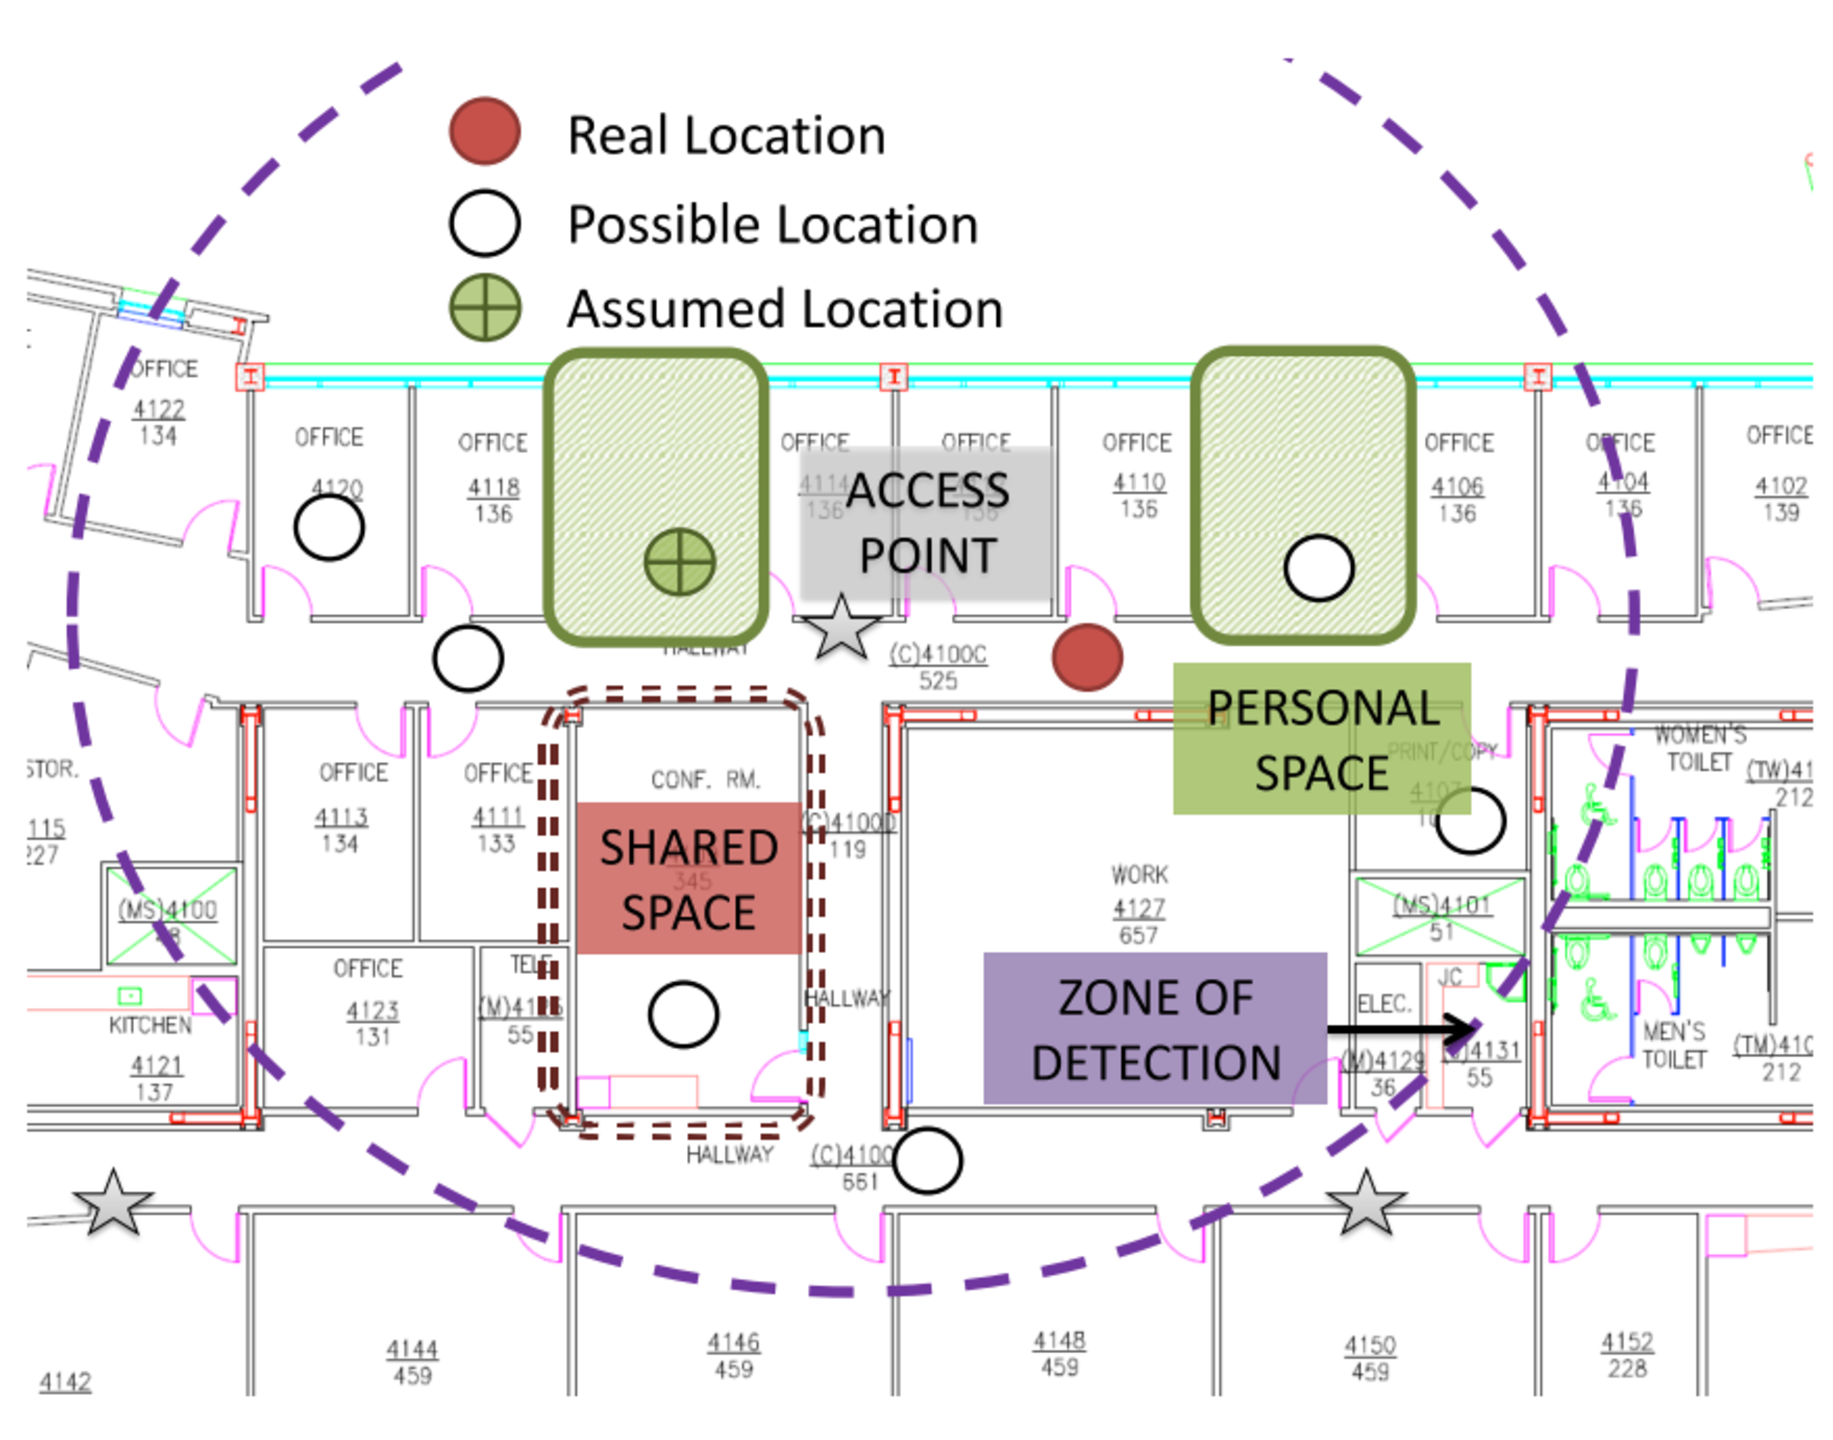
\includegraphics[width=0.6\linewidth]{sentinel.pdf}
\caption[Occupancy inference of the Sentinel system using WiFi connectivity]{Occupancy inference of the Sentinel system using WiFi connectivity. The occupant is assumed to be in her personal space whenever she is within the associated AP’s zone of detection, as denoted by “Assumed Location”.}
\label{fig:sentinel}
\end{figure}

Since an occupant can have different WiFi devices, Balaji et al. decided to use the smartphone as the most representative of the user position. However, the algorithm that they implemented in order to distinguish the phone from the others devices in APs logs has a high level of inaccuracy, causing a degradation of overall results. In addition, smartphones revealed an aggressive sleep policy on WiFi activity as soon as the screen is locked, determining lack of packets and significant false negative detections of occupancy.

\medskip
Implicit sensing solutions have very low costs of installation and don't require the user to do anything except their usual activity. Implicit sensing is usually characterized by low levels of accuracy and resolution; for example can be difficult, if not impossible, to distinguish if more than one connected devices belong to a single occupant of the building. Due to the low performances, implicit sensing is not a suitable source of information for real-time applications like appliance control or safety operations, but thanks to the easy and inexpensive implementation can be always used to collect historical data and to extract long-term occupancy probabilities as a function of time.

\subsection{Ambient Sensor Networks}
\label{subsec:ambient}
Thanks to the diffusion of low cost and low power sensors, and the emerging research area on Wireless Sensor Networks (WSN), solutions based on ambient sensing are currently deeply investigated.
The basic idea is that human presence inside the building continuously affects ambient factors like temperature, humidity, sound, CO\(_2\) and so on. By monitoring these factors the system can estimate the number of occupants.
At this purpose, sensor motes are applied to each room of the building; data is sent to a centralized system where an algorithm estimates the number of occupants. One of the main issues of this approach is the long training period required to build the model, causing time consuming and intrusive data collection. We report two works that tried to overcome this issue.

\smallskip
Beltran et al. proposed ThermoSense \cite{Beltran2013}, a wireless sensor network of nodes that can measure occupancy of rooms. Each node implements a combination of thermal sensor array and PIR sensor. Since occupants are typically warmer than the surroundings, the thermal sensor array, that is capable of measuring multiple temperatures with an area, is used for detecting occupancy. For distinguish between people from passive warm objects, the PIR functionality is exploited. If the PIR sensor indicates the room is empty, then the array determines the thermal background of the space, otherwise the system tries to recognize the number of hotspot corresponding to occupants.\\
The thermal sensor array used is able to measure temperatures in an 8x8 grid pattern within an 2.5mx2.5m area, when placed at a height of 3m (ceiling). A photo of the employed sensor mote and the resulting detection is reported in figure \ref{fig:thermosense}. The system was able to measure occupancy with a Root Mean Square Error of 0.35 person. The weak point of this implementation relies on the short coverage of single sensors, that heavily increases the cost of installation. In order to fully cover a simple 10mx10m room, 16 nodes would be necessary. Covering only hot points like desktop stations or cubicles would drastically reduce the accuracy.

\begin{figure*}
\center
\minipage{0.5\textwidth}
  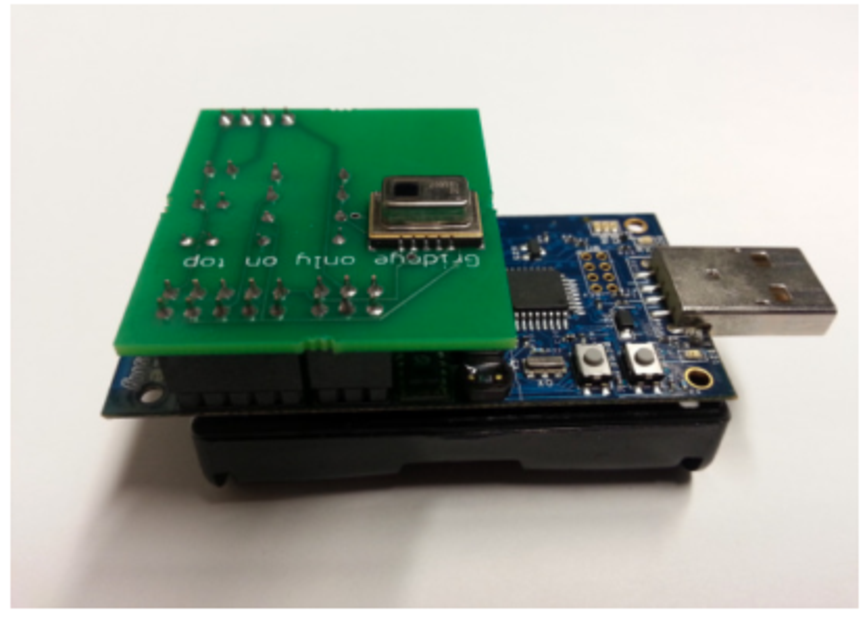
\includegraphics[width=\linewidth]{thermosense1.pdf}
\endminipage\hfill
\minipage{0.5\textwidth}
\center
  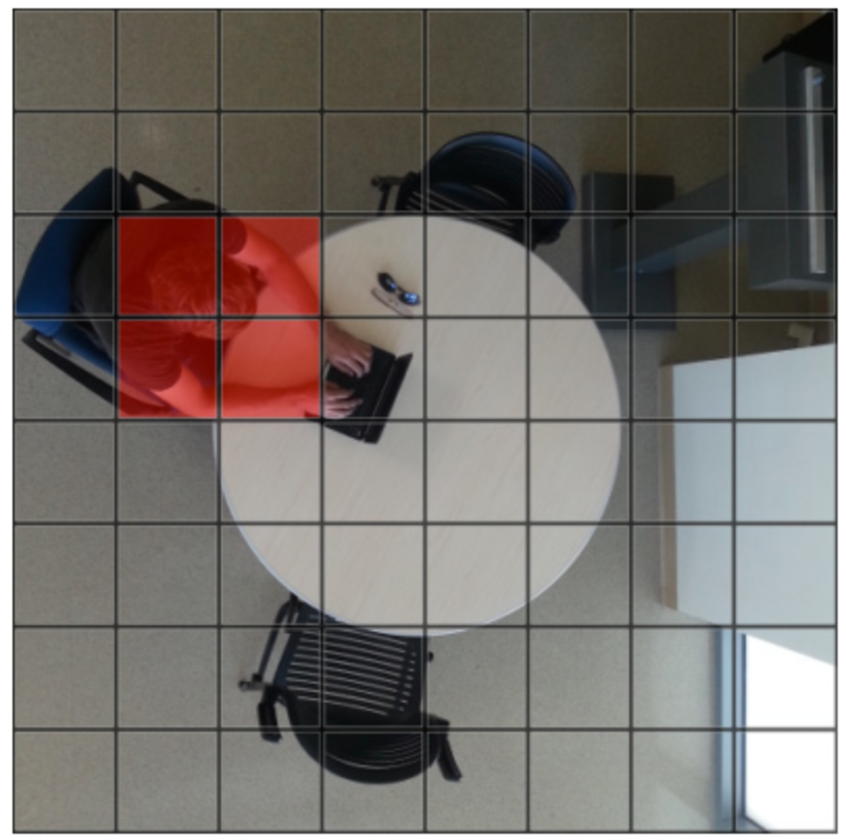
\includegraphics[width=0.8\linewidth]{thermosense2.pdf}
\endminipage
\caption{Thermal sensor array employed in the ThermoSense system and its occupancy detection outcome.}\label{fig:thermosense}
\end{figure*}

\smallskip
Zheng et al. \cite{Cossio2012} proposed a framework for cross-space occupancy modeling in which the model is trained in a space only a single time, and then applied to other geometrically similar spaces. The objective of their study was to generalize relationships between occupancy and ambient factors, collected through sensor boxes equipped with several different sensors: light, sound, motion, CO2, temperature, humidity, PIR and door switch. Training data has been collected from six rooms for long periods of time (10 / 18 months). The occupancy ground truth was collected using ceiling-mounted cameras, which captured images every 10 seconds. Occupancy was then manually labeled for the ground truth. After a phase of selection and pre-processing, the ambient features were used by five supervised learning classifiers to build the general model.\\
The occupancy model was then tested applying samples from other geometrically similar rooms. The modeled occupancy was compared with the actual occupancy detection from 6:00 AM to 9:00 PM (only weekdays) to calculate the performance. They experienced a daily F-measure from \numrange{0.71}{0.94} and a daily RMSE from \numrange{0.42}{1.72} person. However, training rooms employed accommodate no more than four occupants, suggesting that the performances of such model could drastically drop if applied to more populated areas.

\medskip
The advantage of similar solutions is that the user is not forced to keep devices with him/her to be detected by the system. Intrusiveness on the occupant is rather low, except for the employment of cameras and microphones that strongly reduce the privacy.\\
The principal issue of ambient sensing solutions is that ambient factors variate slowly, and provide fast reactions to users movements is difficult. Second, ambient models requires long training period in order to teach the algorithm the relationships between occupancy and ambient factors.
Other complications arise because ambient factors are influenced, besides occupancy, also by HVAC and lighting systems. HVAC and lighting are often the appliances that occupancy detection outputs should regulate, creating undesired feedbacks in the control system.

\subsection{Cameras}
\label{subsec:cameras}
Cameras can be used for measuring occupancy exploiting image analysis algorithms, that recognize bodies or faces within captured images.

\smallskip
Erickson et al. developed OPTNet \cite{Erickson2013}, an occupancy estimation system comprised of 22 node wireless camera nodes used as an optical turnstile to measure area/zone occupancies. They employed a lightweight on-board image processing algorithm along with classification techniques in order to detect occupants' transitions. In addition, they exploited a 40 node PIR wireless sensor network to improve the system accuracy. Figure \ref{fig:optnet} reports two photos of the deployed camera systems and an example of image analyzed. Their work claims to be capable of detecting occupants transitions with up to 94\% accuracy and that the overall system was able to bound the error of occupancy within 1.83 people on average for their building.

\begin{figure}[h!tb]
\centering
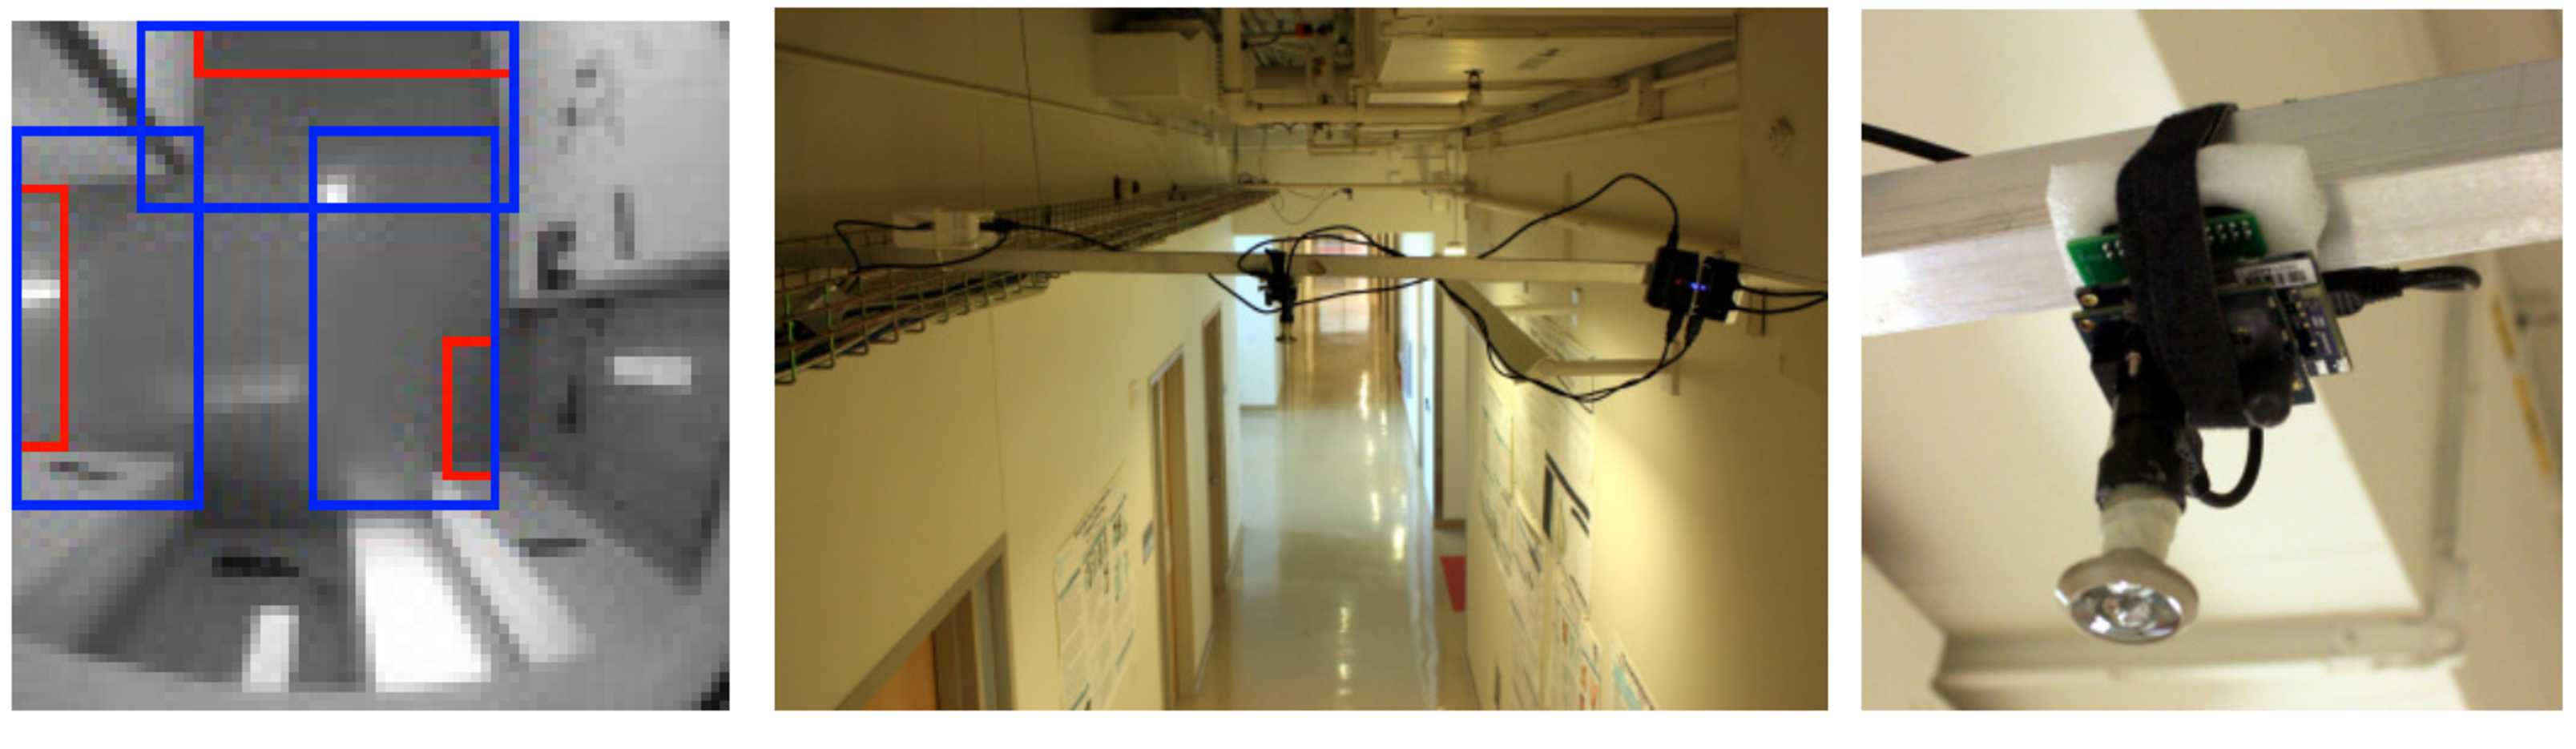
\includegraphics[width=\linewidth]{optnet.pdf}
\caption[The deployed OPTNet system.]{The deployed OPTNet system. Transition areas are represented as bigger blue boxes while trigger areas are small red boxes.}
\label{fig:optnet}
\end{figure}

\medskip
Camera placement is a considerable issue. Cameras placed in offices or meeting rooms raise privacy concerns. A flexible solution for different privacy requirements (and legislations) should allow to keep track of anonymous occupants without collects sensitive data like faces pictures. Cameras can be placed in public and narrow transition points, like hallways or stairways and function as an "optical" turnstile, counting people for each direction. This strategy however is prone to cumulative error: If an optical turnstile misses even a single person entering/exiting a space, this error is propagated until another offsetting error occurs or some other mechanism is used to remove the cumulative error. To give an example, if the last person in an office leaves at 7 p.m. and this transition is missed, then the space will continue to be erroneously considered occupied.\\
Another problem of camera based systems is the computational effort required by the image analysis algorithms. One of the main purpose of smart buildings is the reduction of costs through energy harvesting. In this perspective, the installation of expensive hardware with high computational resources and consumptions for image processing is not the most appealing solution.

\section{Wireless Indoor Positioning}
\label{sec:wips}

In order to determine the position of a user (or an object) in a limited physical space, positioning systems based on wireless technologies have been studied and employed from many years.
Wireless positioning systems, even with deeply different implementation technologies, always rely on a set of reference nodes that communicates with the target object to be localized through generic radio frequency signals.
GPS as instance, the well-known Global Positioning Systems, is able to provides location information anywhere on the Earth where there is an unobstructed line-of-sight with at least four GPS satellites. GPS, which is able to provide good performance levels in open spaces, has been widely adopted for outdoor applications; however, is not capable of operating indoors, due to the significant attenuation introduced by buildings walls and ceilings.

\smallskip
During last years, solutions for indoor localization have been proposed; in this case reference points are represented by WiFi access points or beacons enabled with different signal protocols like Bluetooth.
Some existing solutions that exploit WiFi infrastructure have already been discussed in section \ref{subsec:implicit}. In that case however, the location estimation was performed based on access points data like MAC or IP addresses collected at the Network layer of the OSI model. In this section instead will be discussed localization techniques that analyze the wireless signals at a lower level (Physical OSI layer). For this reason, this section provides first some background concepts of radio signals, later an overview of the most common localization techniques based on signal analysis and finally some relevant related works.

\subsection{Signal Transmission}
\label{subsec:sig_tx}
Electromagnetic signals are classified according to their frequency. Radio frequency (RF) includes all the wave frequencies that lie in the range extending from around 3 kHz to 300 GHz, which include those frequencies used for the most common wireless communications. For this reason the term \emph{Radio Frequency} (or its abbreviation RF) is used as a synonym for radio, describing the use of wireless communication as opposed to communication via electric wires.

The signal transmitted by an antenna can be expressed as a function of time:


\begin{equation}\label{eq:sig_func}
s(t) = a(t) \cos [2 \pi f_c t + \theta(t)]
\end{equation}

where $\theta(t)$ is the phase, $f_c$ is the carrier frequency. A useful measurement of radio signals is power, or more precisely the average power, defined as the time average of energy:

\begin{equation}\label{eq:sig_power}
P = \lim_{T \to +\infty} \frac{1}{2T} \int\limits_{-T}^{+T} (|s(t)|)^2 dt
\end{equation}

When an antenna transmits a RF signal, the signal is characterized by a certain power. The signal at this point is transformed by the antenna into a electromagnetic wave. During propagation the signal travels a medium that introduces some power attenuation to the signal. When the signal hits the receiving antenna this attenuation, also called \emph{Path Loss}, can be expressed as:

\begin{equation}\label{eq:path_loss}
PL = \frac{P_t}{P_r}
\end{equation}

where $P_t$ is the power of the transmitted signal while $P_r$ refers to receiving signal. Different transmission mediums, like free space, air, walls or bodies, can introduce different attenuations. In free space the attenuation is minimal and is in fact called free-space loss. In other materials additional attenuation is introduced by effects like refraction, diffraction, reflection, and absorption. If the medium is completely composed by the free space or the air, the transmission link is referred as Line of Sight (LOS). Differently, if the signal needs to travel across other materials in order to reach the receiving antenna, the communication is called Non Line of Sight (NLOS).

Usually the path loss is expressed in decibels (dB):

\begin{equation}\label{eq:path_loss_db}
PL_{db} = 10\log_{10}(\frac{P_t}{P_r})
\end{equation}

dB unit is a shorthand way to express the ratio of two values. To express absolute values instead, in this thesis many examples and results are expressed in dBm (Decibel-milliwatt), as returned by smartphones and sensors used for the measurements.
The unit dBm denotes an absolute power level measured in decibels and referenced to 1 milliwatt (mW). Absolute power $P$ (in watts) is converted to dBm with the formula $P_{dBm} = 10 \log (\frac{P}{1 mW})$. This equation looks almost the same as that for the dB, except that the power level $P$ has been referenced to 1 mW.

The transmission medium entails, other than the power loss of the signal, also a propagation delay. In particular, the delay depends mainly on the distance to be traveled, and secondary by the wave propagation speed of the medium. For wireless communication this propagation speed tends to $3*10^{8}$, which is equal to the speed of light in vacuum.

\subsection{Signal Analysis for Localization}
\label{subsec:sig_techniques}

Radio Frequency signals transmitted by reference nodes can be analyzed in order to compute or estimate the position of a target object or subject. Different signal characteristics has been measured at this purpose.

\begin{itemize}
\item \textbf{Time of Flight (ToF)}: As we previously said, the time a signal spend traveling from transmitter to receiver depends on the path length and the materials encountered. However, in most cases the main medium is the air and its propagation speed can be considered in good approximation equal to the constant speed in space. ToF technique exploits the resulting linear relationship between travel time and distance, computing distance between two points using the time delay between the transmitted waves.

There are two main approaches to compute ToF, \emph{single packet} and \emph{double packet}. The first simply requires that the reference nodes transmit a packet containing the timestamp of the transmission instant. The receiving mobile device estimates the distance between each nodes comparing the received timestamp with its time of arrival. However this approach requires a strong synchronization between the reference nodes and the target device.
When synchronization between reference and target nodes is impossible or too difficult to achieve, a double packet approach can still be used to determine ToF, as shown in figure \ref{fig:ToF}. This approach is based on the differential time difference of arrival, and eliminates time offsets between the reference and target nodes simply assuming that the path traveled by each packet is the same. Since the same time offset is added to the measured
time of one packet and subtracted from the other, the correct time of flight can be calculated without any synchronization with the equation:

\begin{equation}\label{eq:ToF}
ToF = \frac{T_{b1} - T_{a1} + T_{a2} - T_{b2}}{2} 
\end{equation}

Where $T_{a}$ and $T_{b}$ represent a timestamp measured using respectively node A and B local clocks.

\begin{figure}[h!tb]
\centering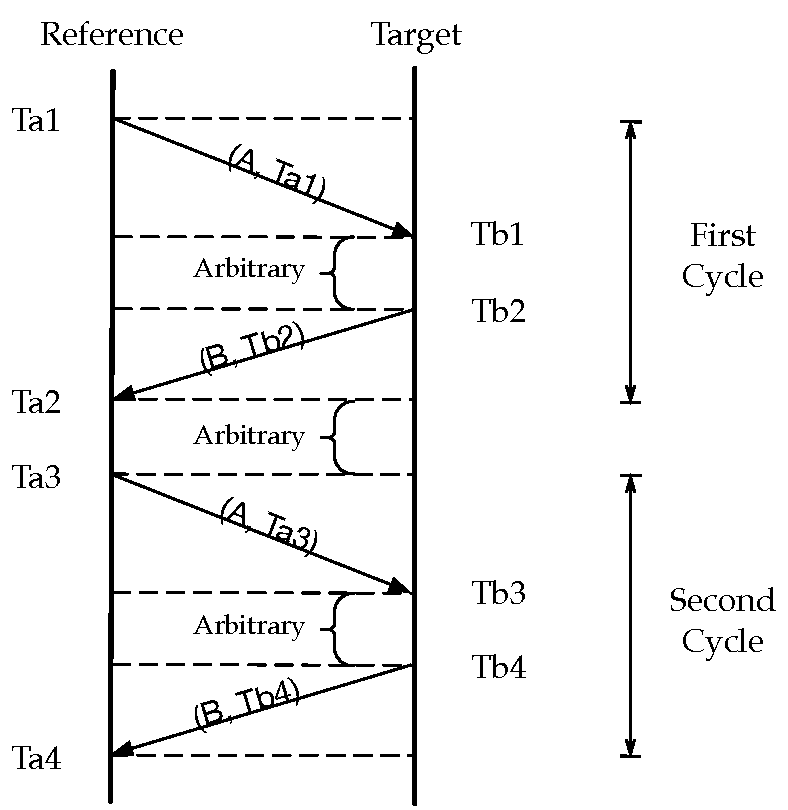
\includegraphics[scale=0.56]{ToF.pdf}
\caption{Time of Flight computation exploiting a double packet transmission.}
\label{fig:ToF}
\end{figure}

\item \textbf{Received Signal Strength Indicator (RSS or RSSI)}: is a measurement of the power present in a received radio signal. RSS can be used in two main approaches: distance estimation and fingerprinting. As introduced in \ref{subsec:sig_tx}, power loss of the signal during transmission depends on the distance, other than the medium material. The RSS perceived by a receiving node from a transmitter can be used to estimate their distance. Typically this estimation requires a prior work to be done before localization can take place. A common necessary training consists in a calibration that measures the RSS value at a fixed distance. Defining $C$ as the received signal strength collected at one meter, the run-time distance can be estimated with the following equations:

\begin{equation}\label{eq:RSS_dist}
RSS_{dBm} = -10 \alpha \log_{10}(distance) + C)
\end{equation}

\begin{equation}\label{eq:dist_RSS}
distance = 10^{\frac{(RSS - C)}{(-10 - \alpha)}}
\end{equation}

Once that three or more distances between reference and target nodes have been computed, the position can be estimated using geometric properties like trilateration.

RSS values can also be used for localization without the needs of estimating each single distance between reference and target nodes, focusing instead on the aggregate RSS information. Pattern Recognition (PR) or fingerprinting techniques attempt to engage a received power levels vector obtained from multiple reference nodes with a defined calibration test, once a time without the need for geometric algorithms. Some example of these pattern recognition techniques, that will be illustrated in the next section, are K-Nearest Neighbors (KNN), Bayesian methods, and Support Vector Machines (SVM).

Depending on OS and application, signal strength is measured either as quality in percentage, or an RSSI value in dBm. RSS values usually range from 0 (zero) to -110dBm and the closer they are to zero, the stronger the signal is. RSS level lower than -80dBm may not be usable for telecommunication, but still very useful for localization.

\item \textbf{Angle of Arrival (AoA)}: is a method for measuring the propagation direction of a RF signal incident on an antenna array. Usually AoA determines the direction by measuring the time difference of arrival at each single antenna of the array, or directly measures the angle exploiting highly directional sensors. Once that angles have been measured, position con be computed using geometric properties of triangles like in the case of RSS, but using triangulation instead of trilateration.

\end{itemize}

\subsection{Localization Techniques and Algorithms}
\label{subsec:loc_algorithms}
In the previous section there have been mentioned some properties and characteristics of wireless signals useful to infer or compute the target position. The way in which these signal properties are used to extract location encompass different algorithms and techniques. These algorithms can be classified in two main classes: \emph{Geometric} and \emph{Fingerprinting}.

Geometric algorithms are based on geometric properties of triangles. They achieve high accuracy localization, provided that the underline signal analysis is also accurate. Their biggest drawback is that they require a meticulous set-up in which distances (or angles) between the installed reference points are precisely measured in order to identify each reference at least in a Cartesian plane, if not in space. Some of the most common geometric techniques are reported below.

\begin{itemize}
\item \textbf{Trilateration}: is the process of determining absolute or relative locations of points by measurement of distances between reference and target nodes, using the geometry of circles, triangles, or spheres. Representing the space in two dimensions, when receiving a signal from a single transmitter, target device can be situated on a circumference with the reference at the center. With two transmitters there are only two positions possible: the two points where the circles around the two transmitters intersect. Adding a third transmitter enables to eliminate one of these two possibilities.
In figure \ref{fig:trilateration}, this condition is represented by a target node T localized by means of distances $d1, d2, d3$.

\begin{figure}[h!tb]
\centering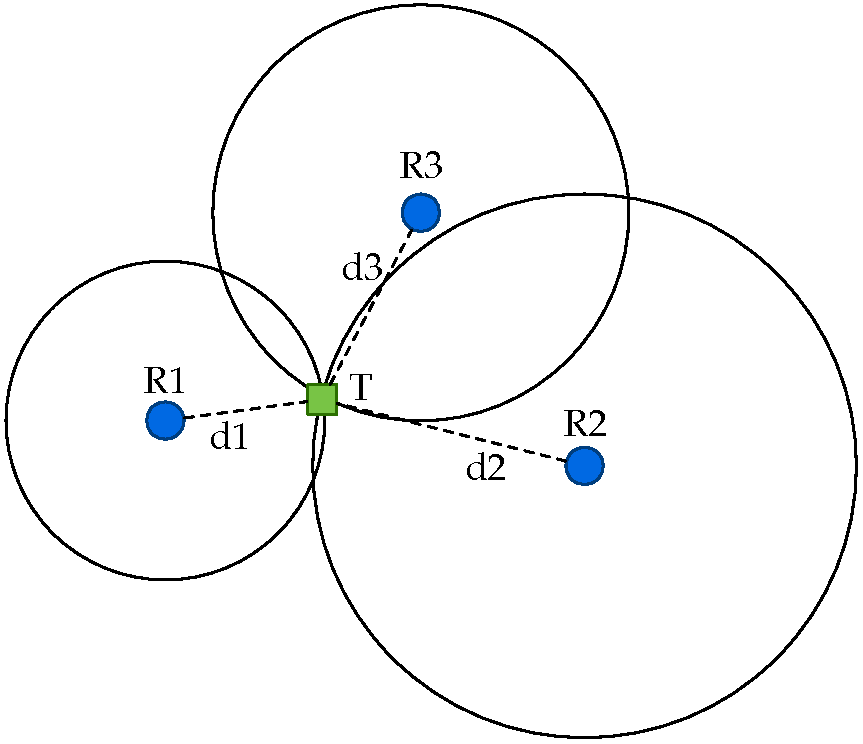
\includegraphics[scale=0.45]{trilateration.pdf}
\caption{Example of a target node $T$ localized with Trilateration by means of distances $d1, d2, d3$.}
\label{fig:trilateration}
\end{figure}

When we extend trilateration to three dimensions, the circles become spheres. In this case it's necessary to add one additional transmitter in order to find the position of the target. This explains why GPS needs to receive at least four satellites to work.

\item \textbf{Triangulation}: allows an observer (target) to calculate its position by measuring two directions towards two reference points. Since the positions of the reference points are known, it is hence possible to construct a triangle where one of the sides and two of the angles are known, with the observer at the third point. This information is enough to define the triangle completely and hence deduce the coordinates of the observer. An example of the triangle construction is reported in figure \ref{fig:triangulation} where the system is able to measure at run time $\alpha$ and $\beta$, while distance $L$ is known since the two reference points $R1$ and $R2$ have well-known coordinates.

\begin{figure}[h!tb]
\centering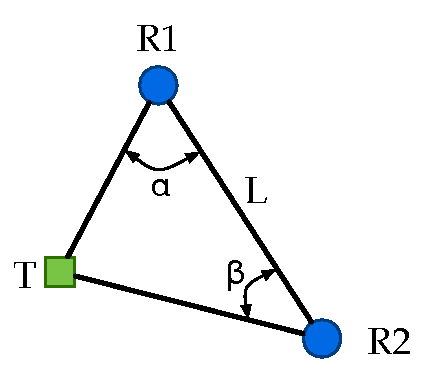
\includegraphics[scale=0.6]{triangulation.pdf}
\caption[Example of Triangulation of a target node $T$]{Example of Triangulation where the system is able to measure at run time $\alpha$ and $\beta$, while distance $L$ is known since the two reference points R1 and R2 have well-known coordinates.}
\label{fig:triangulation}
\end{figure}


\item \textbf{Min-Max algorithm}: is based on simple geometric considerations, and it is one of the most used for localization due to its easy implementation. The target node computes the distance $d_i$ from each reference node, and for each of them it draws a square with center in the position of the reference node, and edges of length $2d_i$. Then, the algorithm calculates the intersection among the squares drawn around the anchor nodes, and the mobile node is at the center of the resulting quadrilateral. In mathematical terms, the target node computes the maximum and minimum values, and it identifies a square having coordinates

\begin{equation}\label{eq:minMax}
(max_{(x_i - d_i)}, max_{(y_i - d_i)}) \times (min_{(x_i - d_i)}, min_{(y_i - d_i)})
\end{equation}

The center of this four-sided figure is the estimated position searched. An example of Min-Max estimation is shown in Figure \ref{fig:minmax}.

\begin{figure}[h!tb]
\centering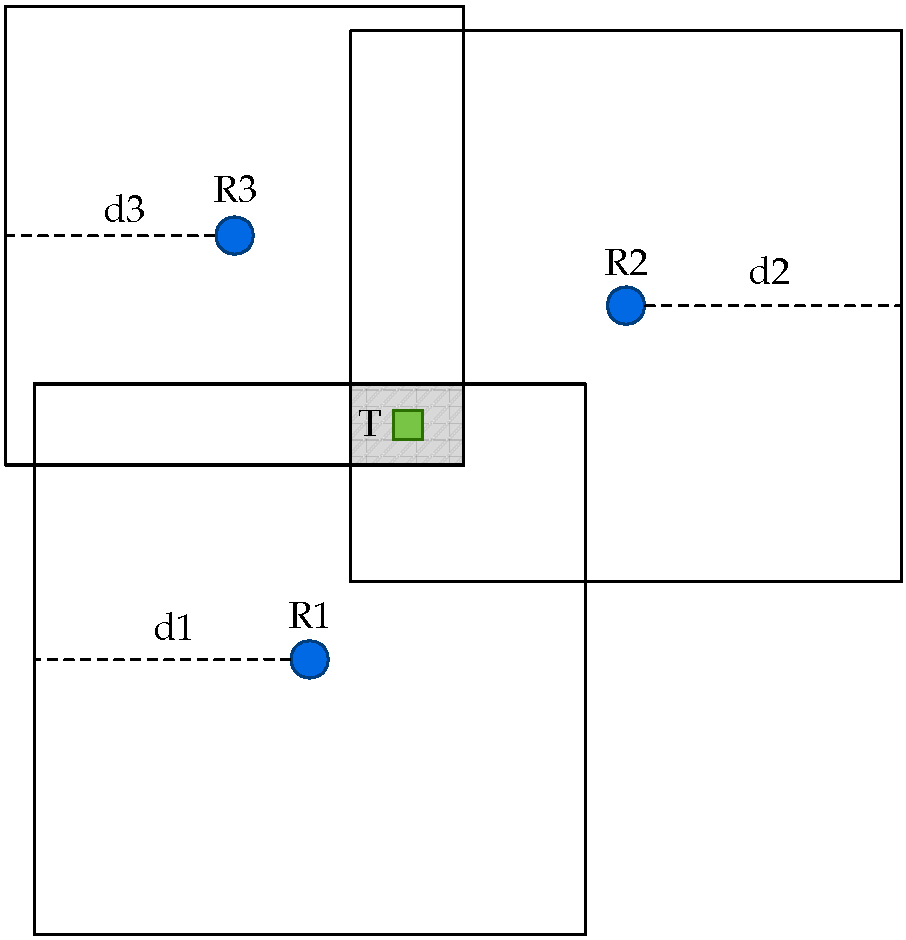
\includegraphics[scale=0.4]{minMax.pdf}
\caption[Example of MinMax computation]{Example of MinMax computation where the target node computes the distance $d_i$ from each reference node, draws a square with center in the reference node and edges of length $2d_i$. }
\label{fig:minmax}
\end{figure}

\item \textbf{Maximum Likelihood Algorithm}: is based on statistical considerations on the set of measures coming from the reference nodes. Its main aim is to minimize the Mean Square Error (MSE) of the measurements which are affected by noise. First, an estimate of distance $d_i$ to each reference device is derived from the RSSI value. Then, the node defines the error $e_i$ between the measured and the actual distance with the following equation:

\begin{equation}\label{eq:maxLike}
e_i(x_0, y_0) = d_i - \sqrt{(x_i - x_0)^2 + (y_i - y_0)^2}
\end{equation}

where $(x_0, y_0)$ is the unknown position of the target node and $(x_i,y_i)$ the position of the $i$-th reference node. To estimate the position this algorithm minimize the MSE, obtaining solutions with low error variance. Unfortunately the measurement pool need to be significant, and with only three reference nodes the accuracy can be poor.
\end{itemize}

%intro fingerprinting
Fingerprinting techniques are used to estimate the position of a mobile device based on measured signal characteristics without the constraints of geometric properties. This subsection will refer to RSS as the main signal measure, but the same could be applied to ToF or AoA. Each target receives the signal from \(k\) nodes, each one with a given power. The values are collected at run-time into a vector of \(k\) element that is later compared with a dataset of vectors, each one pre-labeled with the corresponding position. Although fingerprinting algorithms are less accurate then geometric techniques, they are more flexible since there aren't constraints on the vectors dimension. In addition, training phase are usually far more easy and fast to perform, since to construct the database is sufficient to subdivide the target area in tiles and scan for the surrounding signals in each one of them.
The most common ways in which run time and database vectors are compared to estimate target position are reported below.
\begin{itemize}
\item \textbf{K-Nearest Neighbors (KNN) method}: is based on the idea that even if RSS values do not depend linearly on the distance between references and target, some relation exists. Exploiting this relations, a database of locations and the radio map (the set of test vectors) can be created, containing the position of each location (as coordinates or tile) and the corresponding RSS from the reference nodes. To locate the target device, the vector of current received powers is analyzed, and then compared with the database of locations. The test vector closest to the received one is selected. A majority vote on the vector elements is used to identify the closest test vector. Later, euclidean distance between runtime and off-line vector can be used to adjust and improve the outcome position.
An example has been provided in figure \ref{fig:KNN}. For each room, three signal scans have been performed and are represented by colored shapes. The classification assigns to the runtime measure (green square) the most likely position based on the three closest values.

\begin{figure}[h!tb]
\centering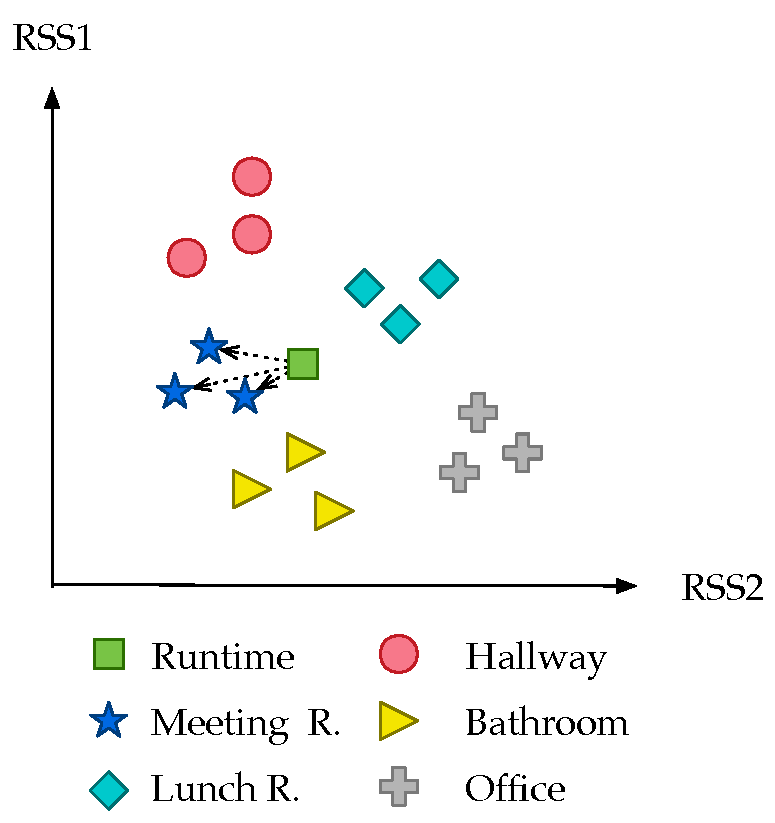
\includegraphics[scale=0.55]{KNN.pdf}
\caption[Example of KNN classification of a position between the target sub-areas]{Example of KNN classification of the current position between the target sub-areas. For each room, three signal scans have been performed. The classification assigns the most likely position based on a majority vote with $K=3$.}
\label{fig:KNN}
\end{figure}

\item \textbf{Bayesian method}: A Bayesian network containing the points of interest is built during the training phase. In the next step the system is trained a certain time on each of the points of interest, collecting RSS samples periodically. During the training phase, a priori probability $p(L)$ is constructed as a function of location L. Then, conditioned posteriori probabilities $p(E|L)$ are defined as the function of perceived RSS from a reference nodes in a certain location, and a given event or locations history (E). These methods are able to model impossible transitions from one location to another, in similar way as in Hidden Markov Model (HMM).

\item \textbf{Support Vector Machines (SVM)}: This method is a paradigm of Neural Networks, in which measure/observation vectors are processed. Processing is done by using a hypothesis space of linear functions over a space with a greater dimension (space of high-dimensional features) where the dimension of observations is induced by a kernel function with the purpose to obtain a hyperplane that separates linearly the observations and let to locate points in the most reliable as possible way. An hyperplane separates the set of training points into two subsets, each one containing a different label. From all possible planes there is only one optimal separating hyperplane (OSH) which is calculated by maximizing the distance between the optimal separation hyperplane and the closest training pattern, i.e. the maximum margin.

\item \textbf{Neural Networks Methods (NN)}: this method uses a Neural Network to estimate the location processing distinct RSS emitted from fixed receptor-emitters. The NN is implemented by a multilayer perceptron in which the input entries may be the RSS of each fixed receptor-emitters, and the output is likely to be in each of the locations.

\end{itemize}


\subsection{WiFi Protocol}
The midrange wireless local area network (WLAN) standard, operating in the 2.4GHz Industrial, Scientific and Medical (ISM) band, has become very popular in public hot-spots and enterprise locations during the last few years. With a typical gross bit rate of 11, 54, or 108 Mbps and a range of 50-100 m, IEEE 802.11 is currently the dominant local wireless networking standard. It is, therefore, appealing to use an existing WLAN infrastructure for indoor location as well, by adding a location server. The accuracy of typical WLAN positioning systems using RSS is approximately 3 to 10 m, with an update rate in the range of few seconds.

All the functionality of the protocol is reflected in the packet headers. RF technology and station mobility impose some complex requirements on 802.11 WLAN networks. This added complexity is reflected in the long physical layer convergence protocol (PLCP) headers as well as the data-rich MAC header. The packet compared with the Ethernet structure is showed in figure \ref{fig:802}.

\begin{figure}[h!tb]
\centering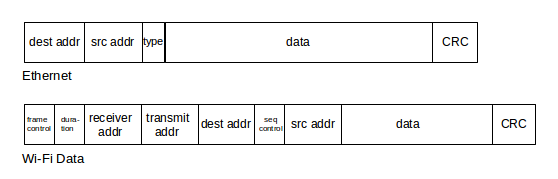
\includegraphics[scale=0.8]{802.png}
\caption{}
\label{fig:802}
\end{figure}

\subsection{Bluetooth Protocol}
Bluetooth is a wireless technology standard for exchanging data over short distances (using short-wavelength UHF radio waves in the ISM band from 2.4 to 2.485 GHz) from fixed and mobile devices, and building personal area networks.
Nowadays, various mobile devices (most of commercially available phones, personal digital assistants, etc.) are equipped with Bluetooth radio transceivers. Due to its broad adoption, Bluetooth can be considered a highly ubiquitous standard. Bluetooth was originally a codename for a project lead by a Special Interest Group (SIG) consisting of major companies, like Ericsson, Intel and Nokia. The Bluetooth bit rate is lower (1 Mbps), and the range is shorter (typically
10-15 m) with respect to Wi-Fi. Moreover, Bluetooth is a lighter standard and supports several other networking services in addition to IP. For positioning, it is suggested to employ received signal strength indications (RSSI), since RSSI decreases with distance between sender and receiver. Since Bluetooth is a low-cost and low-power technology (Bluetooth tags are small size transceivers), it can be intended as an efficient solution to design IPSs. The Bluetooth positioning systems suffer from the same drawbacks of RF positioning technique in complex and full of obstacles indoor situations.


\subsubsection{Bluetooth 4.0 or Bluetooth Low Energy (BLE)}
\label{subsec:BLEprotocol}

Bluetooth v4.0 introduced Bluetooth Low Energy in 2014, officially known as BLE or Bluetooth Smart. This specification introduced a completely different wireless radio that was smaller, cheaper and lower power to meet the needs of these new applications. The wide support for it in smartphones, tablets and embedded systems makes BLE one of the most appealing protocol for the Internet of Things communications.

\smallskip
BLE specification divides Bluetooth devices in two classes: \emph{Central} and \emph{Peripheral} devices. Central devices can scan for other devices and initiate a communication. Usually, the central is a smartphone, tablet or a PC.
Peripheral wait for connections or broadcast unconnected signals coming from sensors. Typically, the slave is a small device like a fitness tracker or a smart-watch that wait for a central device and broadcast the sensed data.
Another type of peripheral device is the Bluetooth beacon, a small devices usually battery powered that continuously broadcast a unique identifier in the surrounding area for ranging applications. Some examples of BLE beacons on the market are the Estimote beacon or the Apple iBeacon.

BLE has two ways of communicating. The first way to communicate is to receive packets using a \emph{Connection}, where both the peripheral and central send packets.
The second way is using \emph{Advertisements}, where a BLE peripheral device broadcasts packets to every device around it. The receiving device can then act on this information or connect to receive more information.
Advertising is by design unidirectional. A Central device can't send any data to the Peripheral device without a connection. But a single peripheral can advertise to multiple masters in the area.

\subsubsection{Apple iBeacon protocol}
\label{subsec:ibeacon}
The iBeacon protocol, since the release of iOS 7, allows a Apple devices to receive push notifications when users enter (or exit) in (from) a iBeacon region. In addition, iOS applications can also evaluate the relative distance among the iBeacons. In iOS, regions associated with an application are continuously tracked, including when the application itself is not running; if a region boundary is crossed, the application is activated in background to handle the event. A possible application of iBeacon is a store where users receive a welcome (plus, eventually, a set of special offers) whenever they enter the store. Usually, in this kind of applications, the accuracy in determining the location of the users is not critical, and even an approximation of several meters can be acceptable.

\subsection{Existing Wireless IPS}
\label{subsec:wips_soa}

In this section the most relevant wireless indoor positioning exploiting WiFi and Bluetooth are reported.

\subsubsection{WiFi IPS}
\label{subsubsec:wifi_soa}

ARIEL \cite{Jiang2012} is a fully automated indoor room localization system. To accurately identify rooms without extensive manual annotation, they developed a number of novel techniques. First, a zone-based clustering algorithm that accurately identifies room occupancy hotspot(s) using Wi-Fi signatures. A clustering algorithm based on motion to identify inter-zone correlation, thereby distinguishing different rooms. An energy efficient motion detection algorithm to minimize the noise of Wi-Fi fingerprints.\\
ARIEL has been implemented and deployed for a 10-month study with 21 participants. The evaluation results demonstrate that their automated clustering algorithm generates clusters that are high representative of individual rooms and achieves high accuracy (95\%) for room localization. The accuracy is comparable to existing techniques that require manual annotation.

Beder and Klepal \cite{Beder2012} focused on the likelihood observation function used in fingerprinting based localization. They proposed two improvements on the commonly used Gaussian approach directly addressing two well-known issues. The first issue was the differing antenna attenuation between different devices, that they addressed by explicitly estimating a global offset thereby considering only relative differences between vectors of received signal strength measurements. The second issue was dealing with environments where not every beacon is visible everywhere, which they proposed to address by explicitly modeling the pickup probability of beacons using Gibbs distributions. Both improvements of the likelihood observation function were shown to increase the performance of their localization system. A suitable distance metric between signal strength measurements is at the core of every fingerprinting based localization system, however their findings are likely to improve all systems currently relying on a purely Gaussian approach.\\
during the 2014 Microsoft Indoor Localization Competition, 22 different solutions to indoor localization from different teams around the world were put to test in the same unfamiliar space, and the system deployed by Beder and Klepal \cite{Beder2012} performed better in the infrastructure-free (WiFi) category.


\subsubsection{Bluetooth IPS}
\label{subsubsec:bt_soa}

Zhu et al. \cite{Zhu2014} proposed one of the most relevant RSSI based Bluetooth positioning method. As usual, there are two phases in their positioning procedure: offline training and online locating. In the phase of offline training, they used piecewise fitting based on the log-normal distribution model to train the propagation model of RSSI for every BLE reference node. They design a Gaussian filter to pre-process the receiving signals in different sampling points. In the phase of online locating, they used weighted sliding window to reduce fluctuations of the real-time signals. In order to reduce the errors of targets coordinates caused by ordinary least squares method, they propose a collaborative localization algorithm based on Taylor series expansion. Another feature of their method is the active learning ability of BLE reference nodes.\\
Every reference node adjusts its pre-trained model according to the received signals from detecting nodes actively and periodically, which improve the accuracy of positioning. Experiments showed that the probability of locating error less than 1.5 meter is higher than 80\%using their positioning method.

Nacci et al. \cite{Conte2014} proposed BlueSentinel, a Bluetooth Low Energy occupancy detection system based on the Apple iBeacon protocol, with the aim to provide an energy efficient solution. In particular they proposed a modification of the iBeacon protocol, still based on BLE, in order to overcome the limitation that allows mobile devices to detect iBeacons only when entering and exiting from beacons proximity. The main idea of their implementation was to change the way the beacons advertise the region associated with them. Instead of correlate each one of them with only a single region, they let the beacons advertise more than one region, in a cyclic sequence. Thanks to this, they was able to create false events that force the operating system to wake up the mobile application more frequently.\\
The application was in charge of computing the position using RSS values and transmitting the location data to the BMS through HTTP requests.\\
The results confirmed that HTTP protocol over WiFi, even if simple to use, is not the best choice when a continuous communication is required. A test performed on a Android device (using HTTP over WiFi) showed that the battery discharged completely in only 4 hours. A different test showed that the energy consumption related to BLE tasks was \numrange{5}{10}\% of the consumption related to WiFI. This demonstrates that true low power state was guaranteed only for the stationary device (beacon) while the mobile device was forced to heavily affect the battery, increasing users effort and intrusiveness. Some consideration on this issue are reported in the next section (\ref{subsec:wips_od}).

\subsection{Indoor Localization for Occupancy Monitoring}
\label{subsec:wips_od}
The problem of monitoring the occupants location in smart buildings can be erroneously considered equal to the more traditional indoor localization problem. Although the same localization algorithms and techniques can be applied, their implementations requires relevant structural differences.

\smallskip
The main purpose of traditional indoor localization systems is to provide to the user its position on the building. The location information is exploited for navigation apps that assist the user moving from a starting point to a destination in the building, or more generally to orient the user in the indoor environment. At this purpose, signal analysis and localization algorithms are always executed on the mobile device.
Scans for wireless signals and location computation usually involve high battery consumption for the mobile devices. However, the mobile energy efficiency is not taken in consideration by the majority of the existing wireless IPS because orientation and navigation tasks are usually executed by users for a limited execution time (typically few minutes) and don't affect the battery lifetime.

\smallskip
Occupancy monitoring for smart buildings shows requirements extremely different. First, the main purpose is to obtain users presence and position information at the infrastructure level. Here the occupancy information can be exploited by the BMS to regulate automatic systems (e.g. HVAC and lighting), build occupancy probability profiles, expose occupancy information to safety applications, and so on.
Since the information is required in real-time on the infrastructure side (back-end), traditional indoor positioning systems that compute location on mobile device needs to transfer the location data through mobile connectivity.

Take in consideration WiFi based IPS as shown in figure \ref{fig:wfips_od}. The mobile device compute its position exploiting signals coming from WiFi access points. In order to monitor its position in real-time, the mobile application needs to upload the current position continuously, generating an interminable connection with high energy consumption (red connection in fig.~\ref{fig:wfips_od}). Since occupancy monitoring is required to work potentially for many hours of the day, the approach become unsustainable for the mobile battery. In addition, an energy-hungry application is intrusive for the user point of view and less likely to be adopted for continuous monitoring.



\begin{figure}
     \centering
     \subfloat[]{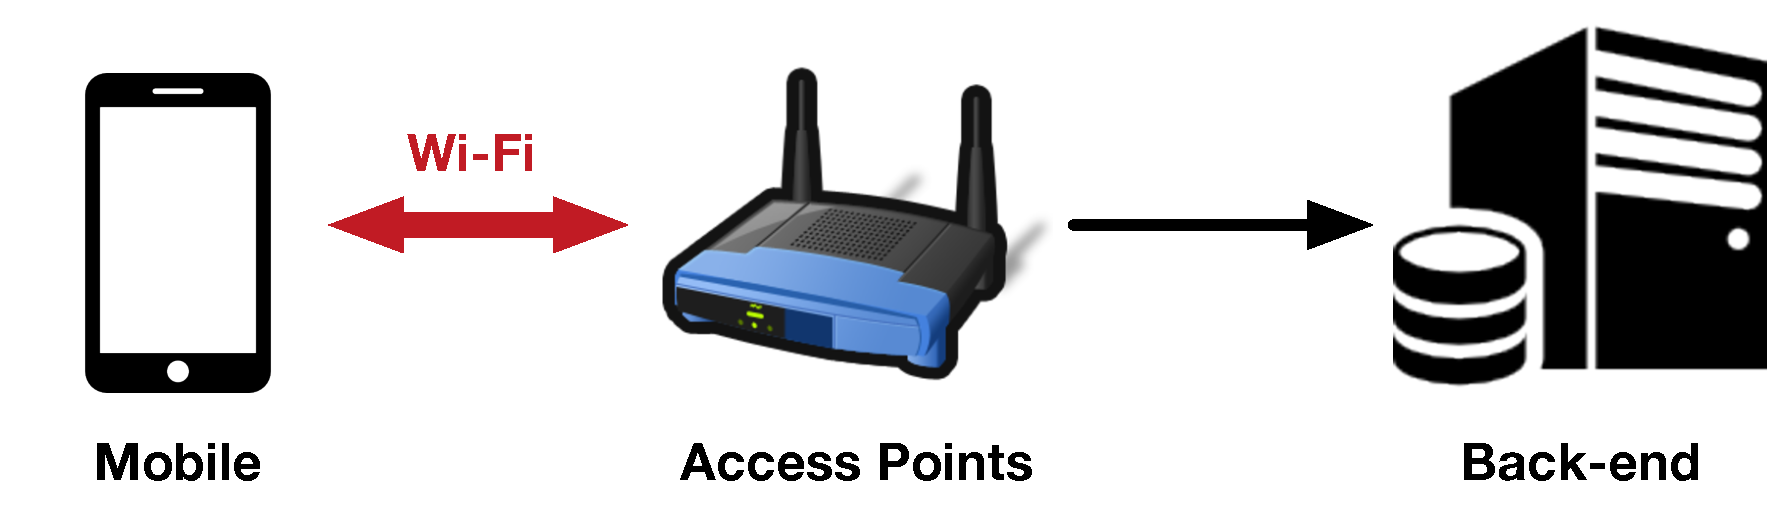
\includegraphics[scale=0.32]{protocololdwf.pdf}\label{fig:wfips_od}}\\[-2ex]
     \subfloat[]{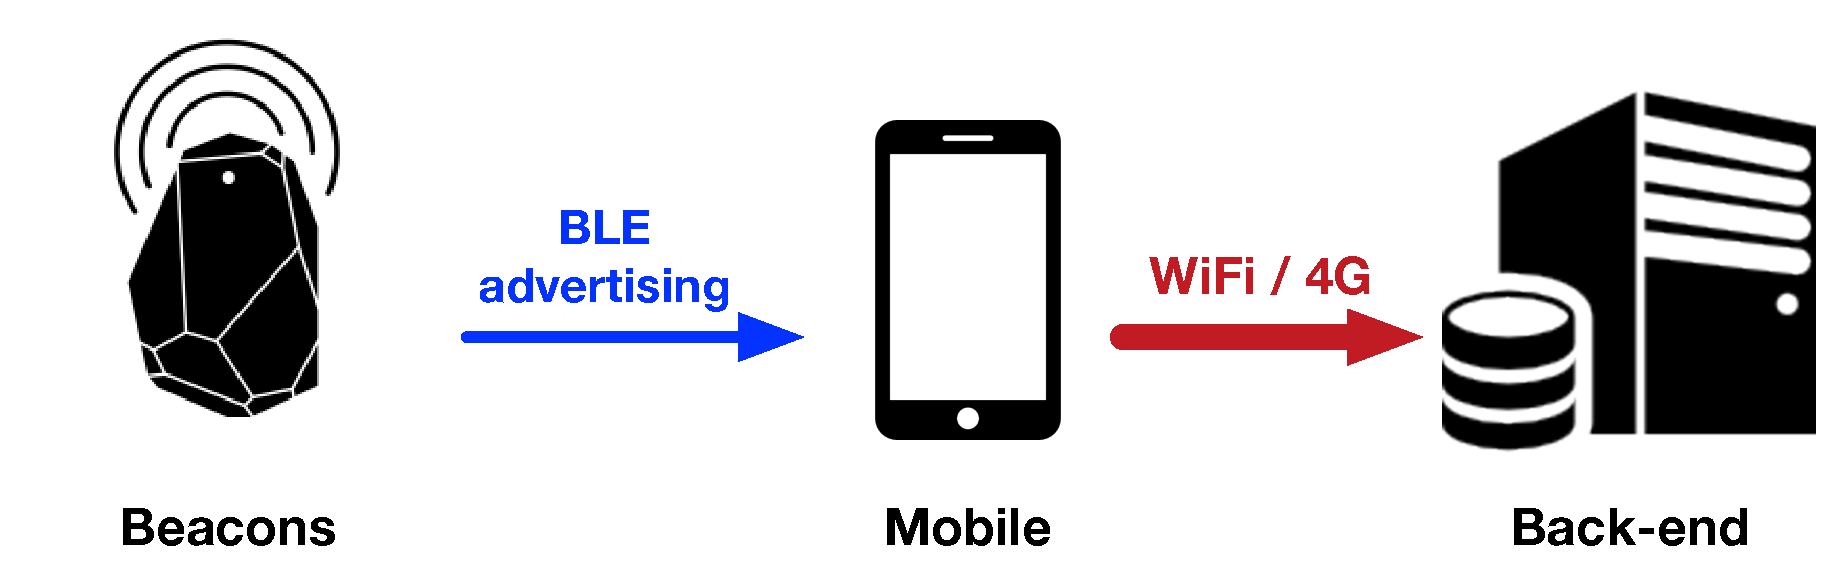
\includegraphics[scale=0.32]{protocololdbt.pdf}\label{fig:btips_od}}
     \caption[Traditional Indoor Positioning Systems applied for occupancy monitoring.]{Traditional Indoor Positioning Systems applied for occupancy monitoring. \protect\subref{fig:wfips_od} Refers to common WiFi based IPS, \protect\subref{fig:btips_od} refers to common Bluetooth based IPS used for real-time monitoring.}
	\label{fig:wfips_btips}
\end{figure}


% \floatsetup[figure]{style=plain, subcapbesideposition=center}
% \begin{figure}
% \centering
% \sidesubfloat[]{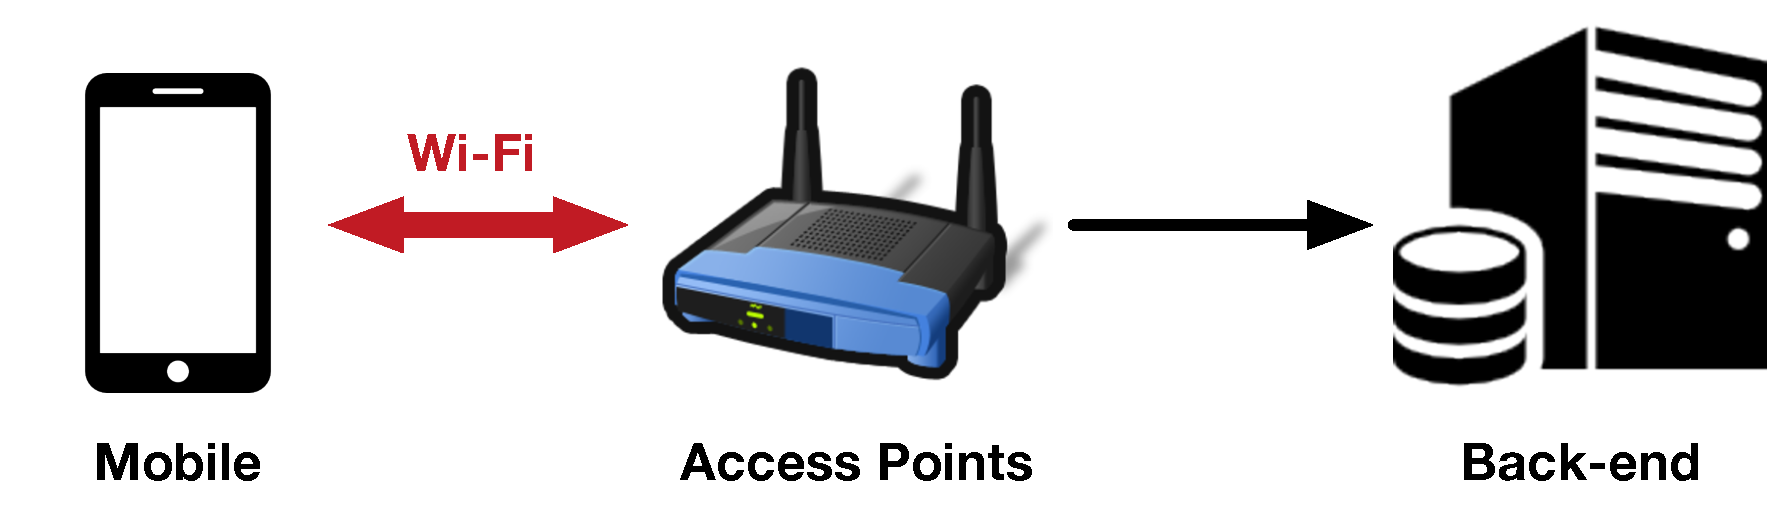
\includegraphics[scale=0.33]{protocololdwf.pdf}\label{fig:wfips_od}}
% \newline
% \sidesubfloat[]{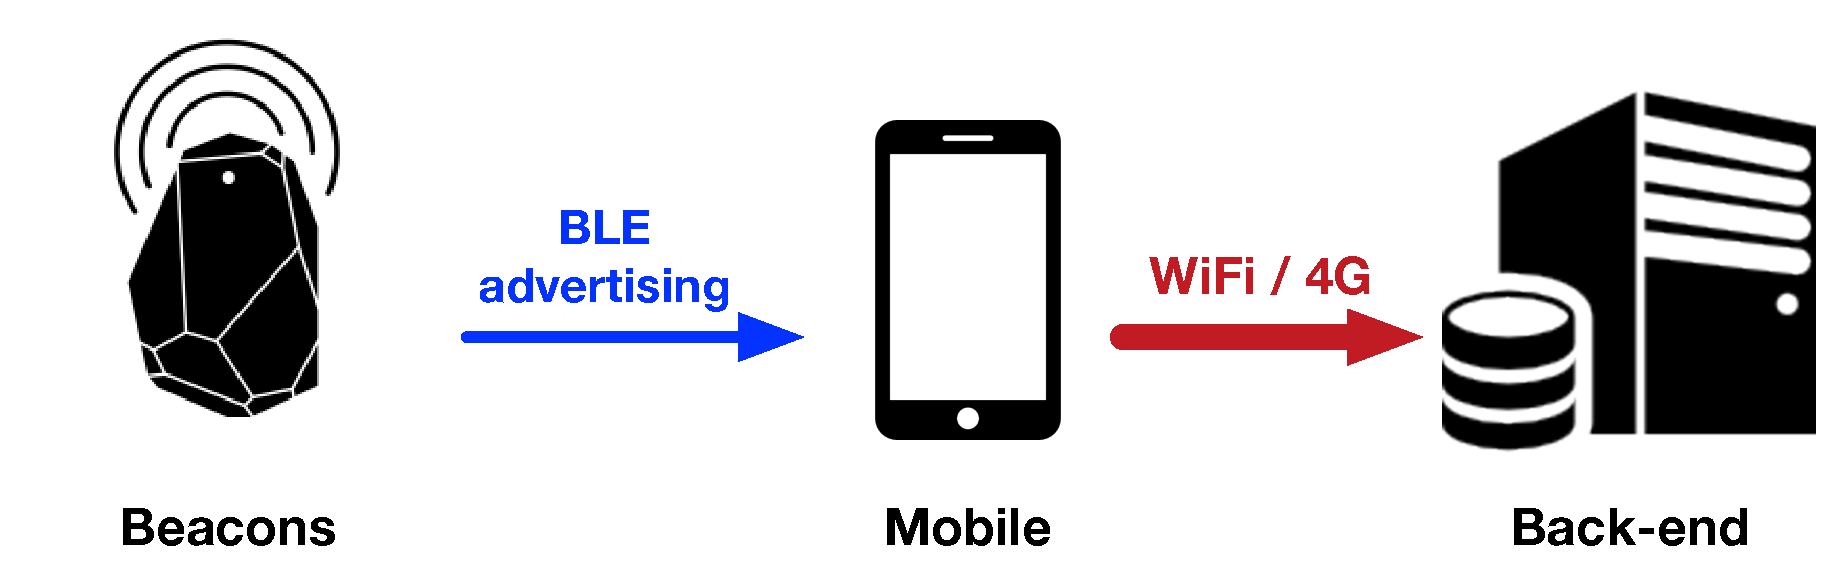
\includegraphics[scale=0.33]{protocololdbt.pdf}\label{fig:btips_od}}
% \caption[Traditional Indoor Positioning Systems applied for occupancy monitoring.]{Traditional Indoor Positioning Systems applied for occupancy monitoring. \protect\subref{fig:wfips_od} Refers to common WiFi based IPS, \protect\subref{fig:btips_od} refers to common Bluetooth based IPS used for real-time monitoring.}
% \label{fig:wfips_btips}
% \end{figure}

In case of Bluetooth Low Energy, the employment of reference nodes such as beacons enable to provide users with their location using a low power communication. The wide popularity of the Apple iBeacon or the Estimote in commercial contexts have proved that BLE beacons are a suitable technology for providing users ranging applications and location aware services. However, in the context of location monitoring, they show the same limitations of WiFi based systems, as reported in figure \ref{fig:btips_od}. In order to retrieve position in real-time at the BMS level, the device needs to send its current position continuously through mobile connectivity, generating a long connection characterized by high energy consumptions.



\section{Comparison}
\label{sec:comparison}

In this last section, all the occupancy detection monitoring systems from existing literature that have been illustrated during this chapter are summarized and compared in table~\ref{tab:od_soa}. Extra devices for building refers to any hardware installation required in common buildings such as offices or schools. WiFi hotspots are considered already present appliances in the building infrastructure. Installation complexity, as defined by Akkaya et al. in \cite{Akkaya2015}, is represented by three tiers from low to high complexity. User intrusiveness is an indicator of how much the its activity is negatively affected by the system. When battery consumption is high, user intrusiveness is also considered high.\\
Accuracy has been considered high if the system was able to localize a user within circumscribed area with an accuracy greater than 85\%. 
%
% ------------------------------------------------------------------------ %
%
\begin{sidewaystable}
%
\caption[Comparison between the most relevant Occupancy Monitoring systems in literature.]{Comparison between the most relevant Occupancy Monitoring systems in literature.}
%
\label{tab:od_soa}
%
\centering
%
\renewcommand{\arraystretch}{0.65}
%
\begin{tabulary}{\textheight}{>{\bfseries}L L L L L L L L L L}
%
\toprule
%
\textbf{Approach} &
	\textbf{Technology}	& \textbf{Extra devices building side}	 & \textbf{Installation complexity}
	& \textbf{Extra device user side} & \textbf{Mobile consumption} & \textbf{User intrusiveness}
	& \textbf{High accuracy} & \textbf{Real-time detection} & \textbf{User identification}\\ 
%
\midrule
%
\cite{Melfi2011}  	& Implicit network sensing & No & Tier \rom{1} & No & None & Very Low & No & No & No\\
%
\cite{Balaji2013}  	& Implicit network sensing & No & Tier \rom{1} & No & None & Very Low & No & No & Yes\\
%
\midrule
%
\cite{Beltran2013}  & Ambient sensors & Yes	& Tier \rom{3} & No & None & Low & No & No & No\\
%
\cite{Cossio2012}   & Ambient sensors & Yes	& Tier \rom{3} & No & None & Low & No & No & No\\
%
\midrule
%
\cite{Erickson2013} & Cameras & Yes	& Tier \rom{2} & No	& None & High & Yes & Yes & No\\
%
\midrule
%
\cite{Jiang2012}  	& WiFi localization	& No & Tier \rom{2} & Yes & High & High & Yes & Yes & Yes\\
%
\cite{Beder2012}  	& WiFi localization	& No & Tier \rom{2} & Yes & High & High & Yes & Yes & Yes\\
%
\cite{Zhu2014}  	& Bluetooth localization & Yes & Tier \rom{2} & Yes & High & High & Yes & Yes & Yes\\
%
\cite{Conte2014}  	& Bluetooth localization & Yes & Tier \rom{2} & Yes	& High & High & Yes & Yes & Yes\\
%
\midrule
%
Proposed approach 	& BLE sensor network & Yes & Tier \rom{2} & Yes & Low & Low & Yes & Yes & Yes\\
%
\bottomrule 
%
\end{tabulary}
%
\end{sidewaystable}



\pagebreak

% Solutions based on wireless technologies have obtained the best results in terms of accuracy, spacial and temporal resolution. They usually make use of common Wi-Fi access points to locate the user's device inside the building.\\
% The most commons approaches use trilateration (Fig~\ref{fig:trilater}), triangulation and time-of-flight techniques. Although these are consolidate and performant techniques in localization (such as GPS systems), they have the drawback to require the exact position of each AP inside the building: the entire floor plan must be measured, as well as the distances between all access points, causing hard and long installations.\\
% In addition, the constant exchange of packets via WiFi is characterized by medium/high power consumption levels, so an employment for many hours of the day can be considered not sustainable for the mobile devices battery and too many intrusive for the user.\\
% An alternative to the WiFi access points are Bluetooth Low Energy (BLE) beacons. A beacon is a small wireless device that constantly broadcasts radio signals to nearby smartphones. This transmission is called \emph{advertising}, and each device advertise a universally unique identifier (UUID). In this way, mobile apps can listen for that signal and, when they receive it, trigger the correct location-based action.
%
% ------------------------------------------------------------------------ %
% !TEX encoding = UTF-8 Unicode
% !TEX TS-program = pdflatex
% !TEX root = ../Tesi.tex
% !TEX spellcheck = it-IT
% ------------------------------------------------------------------------ %
%
% ------------------------------------------------------------------------ %
% 	NOME CAPITOLO
% ------------------------------------------------------------------------ %
%
\chapter[BlueSentinel: the Occupancy Monitoring System]{BlueSentinel: the Proposed Occupancy Monitoring System}
\chaptermark{The BlueSentinel System}
%\markboth{The BlueSentinel System}{The BlueSentinel System}	% headings
%
\label{cap:bluesentinel}

\section{Introduction}
\label{sec:intro}

Smart buildings are environments like offices or schools able to exploit sensors, devices and appliances to observe users activity and adapt autonomously to achieve comfort, safety and energy efficiency. Considering the fast development of technologies for connected sensor and actuator (the so called \emph{Internet of Things}), since few years smart buildings are becoming a reality from a technological point of view.

\medskip
One of the main components of a smart building is the \textbf{Occupancy Monitoring system}, i.e. a system able to detect the number (or even the identity) of the occupants in every room or zone of the building. Occupants play a key role in the objectives of smart buildings. User comfort can be improved controlling automatically the environment temperature, humidity, and brightness, setting all the parameters exploiting user defined preferences. In this scenario, user identification and localization inside the building is fundamental.\\
In order to guarantee the building safety, the knowledge of the occupants position in real-time can be precious. In case of emergencies like fires, escape routes and emergency exits might be highlighted with notifications targeted to the specific user's location.\\
Probably, the main purpose of smart buildings, or in this case also called green buildings, is energy sustainability.
In 2010, heating, ventilation, and air-conditioning (HVAC) consumed 42\% of the energy used in the United States.
At this purpose, in the last few years plenty of methods have been proposed to control HVAC systems based on real-time occupancy information or learning the occupants habits to forecast the energy consumption.

\medskip
The expected outcome of an occupancy monitoring system is the detection in real-time (or with a tolerable delay) of every user inside the building, with their position. Usually, the occupant needs to be localized in a zone or room of the building, since this information is sufficient to automatize HVAC and lighting systems. In cases of automation based on user-defined preferences also the identification of each user is required by the system.

\smallskip
As explained in chapter \ref{cap:soa}, a lot of effort has been put both from the industry and the academia in terms of research and product industrialization. However, some intrinsically hard challenges of the occupancy monitoring problem bring to the lack of an accessible solution with broad adoption.

In this chapter is presented BlueSentinel, an occupancy monitoring system developed with the aim to improve the shortcomings identified in the state of the art.

\section{Choosing the Enabling Technology}
\label{sec:technology}
In the {\hyperref[cap:soa]{previous chapter}}, many possible technological solutions to build indoor location monitoring systems have been reviewed. During the preliminary analysis of our work, all the available technologies have been considered in order to satisfy the occupancy monitoring requirements and a feasible solution for both users and infrastructures.

Considering the comparison summarized in table \ref{tab:od_soa}, it can be deduced that the only solutions able to guarantee a true real-time detection of users are cameras and wireless based solutions. When comparing this two approaches, cameras revealed to have many more drawbacks with respect to wireless solutions.
Camera based systems require a high computational effort to perform real-time body recognition on indoor video (or images) streams. The compute-intensive peculiarity makes the approach not suitable to scale up for large buildings, with tens or thousand rooms and users.
Wireless based solutions tend to provide easily an outcome in real-time, or with a tolerable delay. Raw data produced by wireless systems is usually far more lightweight to process (for example compared to images), making the solution attractive for large indoor areas.

\smallskip
Inside the wireless scope, the choice is restricted to technologies that all users have already available in their mobile devices, so to avoid the employment of additional objects. The first one is certainly WiFi. WiFi based localization solutions have been deeply investigated, also because of WiFi infrastructure is already present in almost all buildings. However, for monitoring purposes, they are not able to provide real-time location data for long execution periods. This issue is explained in detail in section \ref{subsec:wips_od} and summarized here.\\
There exist two ways to localize a mobile device using WiFi connectivity, an \emph{active} and a \emph{passive} method. The active method requires an application installed on mobile device that keeps an active connection with all the surrounding hotspots, and continuously notify collected data using an Internet connection. However, battery consumption related to WiFi operations is too high to reach many hours of execution.\\
The passive method instead doesn't require any installed application on mobile device, but simply exploits WiFi packets sent from devices during their usual activity. Unfortunately, using this approach, is nearly impossible to obtain real-time detection since mobile operating systems apply aggressive sleep policies to WiFi module in order to limit consumptions. A WiFi connected smartphone during sleep can spend several minutes without emits any signal, making the system unresponsive to users movements \cite{Balaji2013}.

\smallskip
The remaining available wireless technology is Bluetooth, and in particular Bluetooth Low Energy. Since 2010, BLE chips (able to work with classic and Low Energy enabled Bluetooth) have been built into in an increasing number of smartphones, tablets or wearables (as instance, Apple has incorporated them in its products since the iPhone 4S in 2011).
Devices using BLE consume ten times less then WiFi and a fraction of the power of classic Bluetooth \cite{Choperena2013}.
However, at the best of our knowledge, BLE has been employed for localization only through passive appliances (like beacons) that leave the burden on the mobile device, forcing it to run positioning algorithms continuously and notify the result through energy-hungry connectivities.
In order to fully exploit energy efficiency of BLE, the proposed system relies on BLE mobile advertisement (section \ref{sec:advertisement}), a particular BLE signal transmission compatible with almost all mobile devices since few years.
%With the diffusion in the last few years of devices enabled with peripheral mode BLE chipset, BLE advertisement becomes possible on mobile devices
%This makes BLE an excellent technology for a real-time positioning solution.


\section{Mobile BLE advertisement}
\label{sec:advertisement}
As explained in section \ref{subsec:BLEprotocol}, BLE specification divides Bluetooth devices in two classes: \emph{Central} and \emph{Peripheral} devices (figure \ref{fig:cent-per}). Peripheral devices generates data, like sensor readings or audio streams, while Central devices consumes it. This BLE specification was intended to classify smartphones and PC as centrals, while accessories as peripherals.

BLE has also two ways of communicating. The first way is establishing a \emph{Connection} between a peripheral and a central device. Every connection however, requires a preliminary pairing phase between the two devices. This makes unfeasible the employment of BLE connections in monitoring applications, since a mobile device (central) would be forced to perform a pairing with every single reference node (peripheral) before monitoring can start.

\begin{figure}[h!tb]
\centering
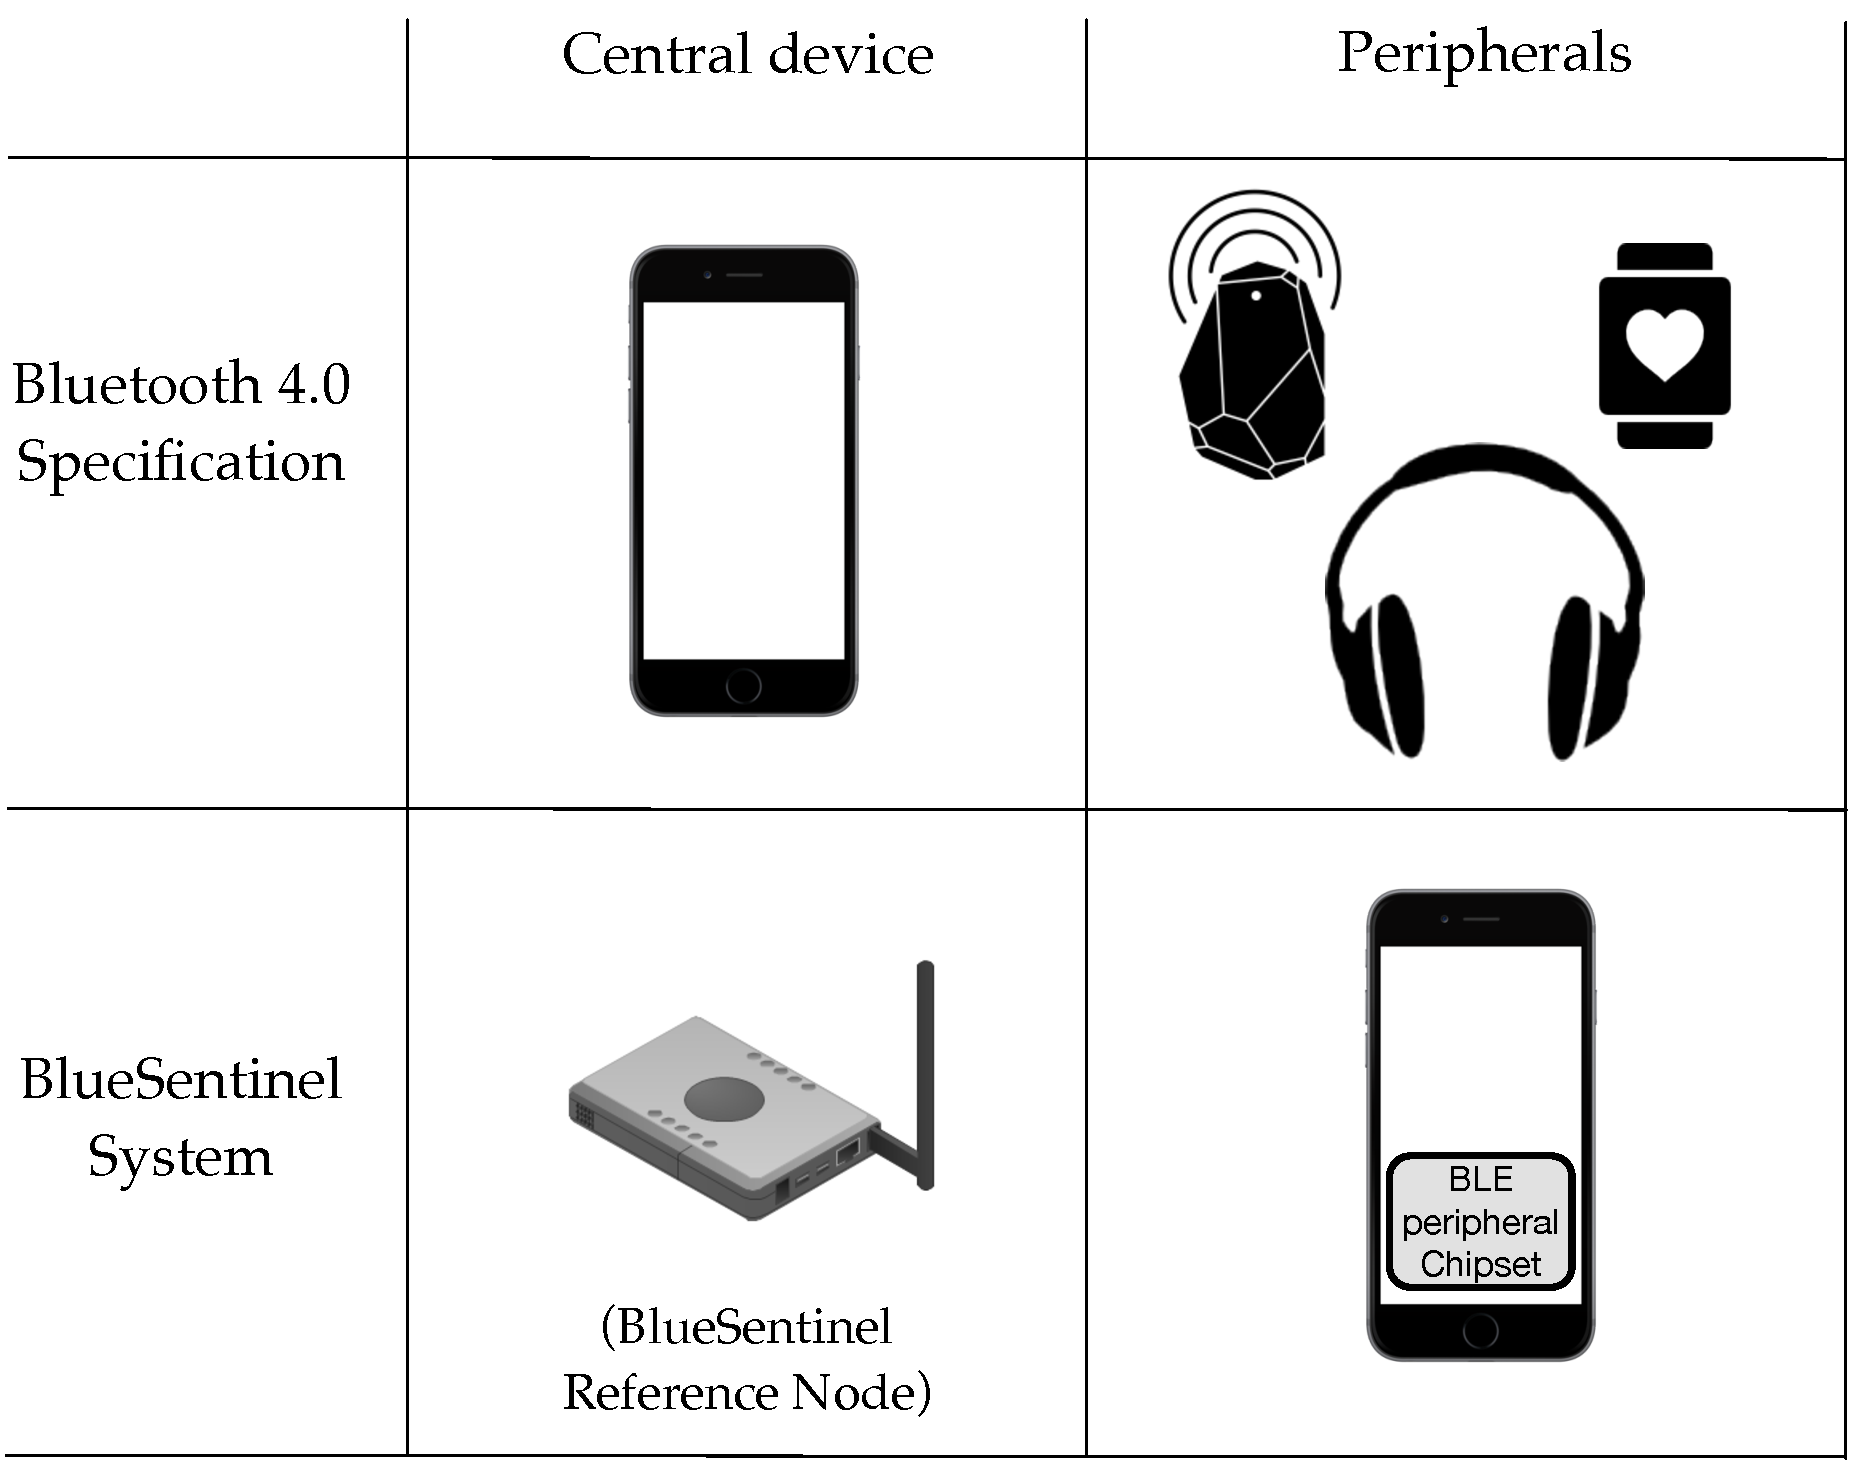
\includegraphics[width=0.8\linewidth]{central-peripheral2.pdf}
\caption[Central and Peripheral devices in BLE specification and the implemented system.]{Central and Peripheral devices in BLE specification compared with the implemented system.}
\label{fig:cent-per}
\end{figure}

The second possible way to communicate is using \emph{Advertisement}, where a BLE peripheral device broadcasts packets to every device around it. The receiving device can then act on this information.
Advertising that is by design unidirectional can be performed exclusively by peripheral devices.
For localization purposes, advertisement devices known as beacons as been employed as reference nodes; however, for localization purposes, this approach leaves the burden on the mobile device, forcing it to run positioning algorithms continuously and notify the result through energy-hungry connectivities (more details in section \ref{subsec:wips_od}).\\
The key idea behind the proposed system is to use smartphones as BLE peripheral devices, while reference nodes as BLE central devices (fig. \ref{fig:cent-per}). In this way, user devices are able to advertise them-self in a given position of the building without any connection or pairing, while reference nodes collect all the received advertisement packets.

\begin{figure}[h!tb]
\centering
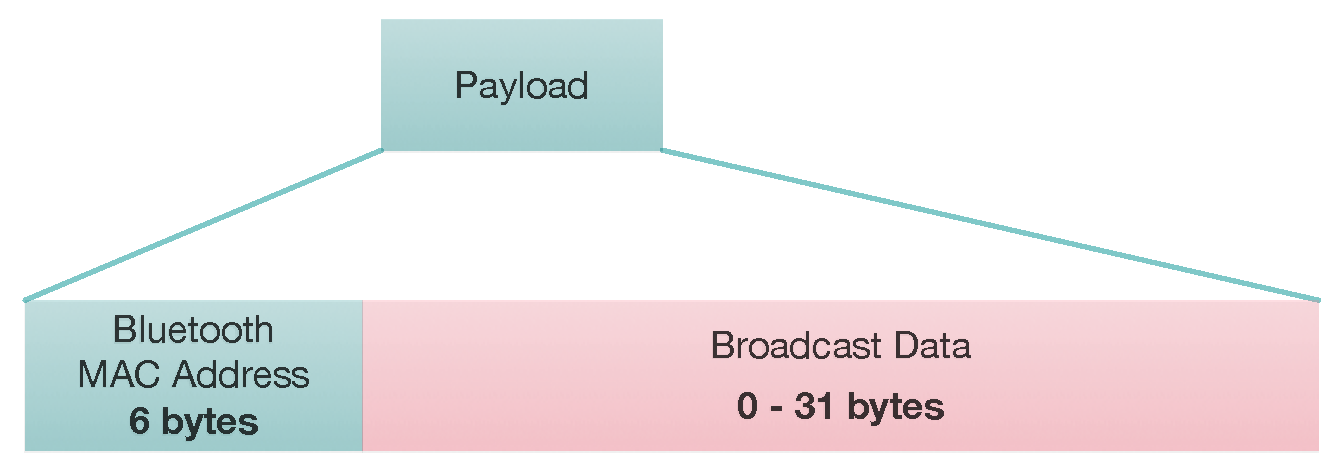
\includegraphics[width=0.65\linewidth]{payload.pdf}
\caption[BLE advertisement packet contents.]{BLE advertisement packet contents.}
\label{fig:payload}
\end{figure}

As shown in figure \ref{fig:payload}, advertisement packets contain the Bluetooth MAC address of the device and a very limited custom payload of 31 bytes. Since we need to identify the user, a straightforward solution would be to associate each MAC address with a registered user. However this is no longer possible on recent versions of Android and iOS since they hide MAC addresses to developers in order to increase user's privacy. For this reason, a Universally Unique IDentifier (UUID) has been employed to recognize each user advertisement.
At the same way in which UUIDs have been used to advertise regions through BLE beacons (like the Apple iBeacon), occupants of a building can be localized and identified in real-time associating each UUID with a building user.

\smallskip
BLE advertisement on mobile devices requires a specific hardware, the BLE peripheral mode chipset. Fortunately, almost all current devices have built-in peripheral chipset: all Apple devices since iPhone 4S and iPad 3, about 80\% of all Android devices released in 2014 and about 90\% in 2015 \cite{RadiusNetwork2016}.
%A Central device can't send any data to the Peripheral device without a connection. But a single peripheral can advertise to multiple masters in the area.

\medskip
The proposed system has been developed using smartphones as advertising devices. However, The same advertising task can be easily implemented on wearable devices like smart-watch, that are natively build as BLE peripheral devices. The employment of wearable devices for occupancy monitoring would be even more effective, since they never separate from their users.

\section{System Overview}
\label{sec:overview}
In this section, the architecture of the proposed system will be over-viewed, while in the next three sections every components will be explained in detail.

The proposed location monitoring system is composed by three main parts (figure \ref{fig:bs-protocol}).

\begin{figure}[h!tb]
\centering
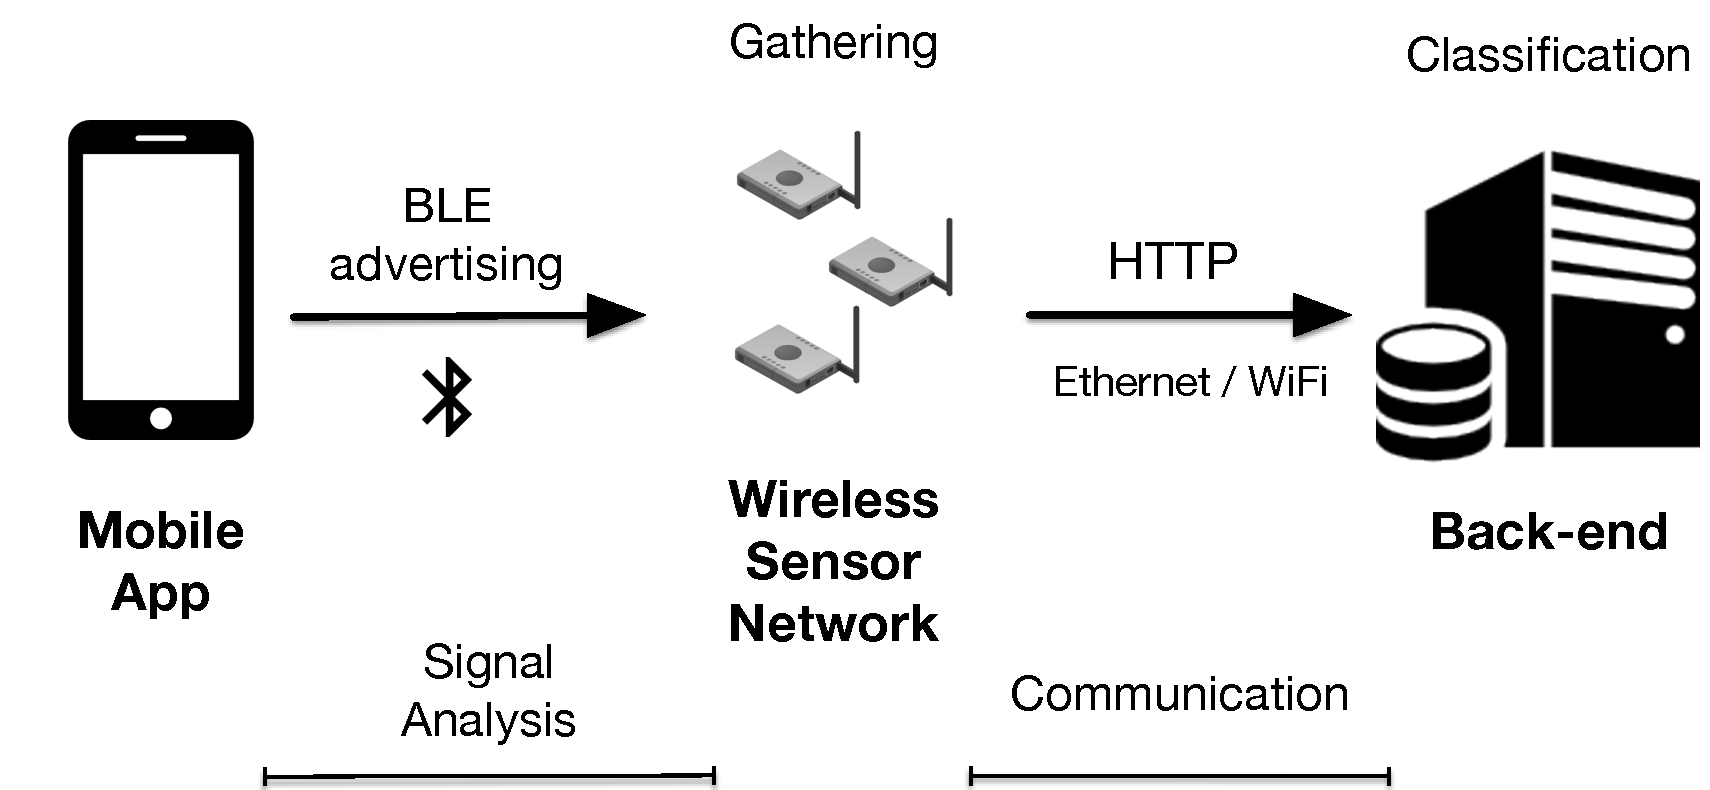
\includegraphics[width=\linewidth]{bs-protocol.pdf}
\caption[Overview of the BlueSentinel occupancy monitoring system.]{Overview of the BlueSentinel occupancy monitoring system. A mobile application perform advertising over BLE. Packets are collected by a network of sensor nodes and analyzed by a centralized system.}
\label{fig:bs-protocol}
\end{figure}

\begin{itemize}
\item First, the \textbf{mobile application} that runs on users mobile devices. The application manages registrations and logins of users (necessary to detect occupants identity) and performs the BLE advertisement. For both Android and iOS devices, it's possible to perform BLE advertisement even during device sleep and when the application is in background.
During BLE advertisement the application is free from any localization algorithm, Internet connection or GPS service, to preserve battery and to bother users as least as possible.

\item The component that directly interacts with occupants mobile devices is a network of Bluetooth Low Energy \textbf{receiver nodes}. This nodes, positioned by the building administrator during the system installation, are in charge of collecting BLE packets coming from occupants, together with signal features (like the received power) useful to estimate their position. The information collected by each node is rapidly forwarded through an Internet connection toward a centralized Building Management System.

\item All the information collected by the sensor nodes are merged at the back-end level by the \textbf{Building Management System} (BMS). Here signal features related to every occupant is reconstructed and compared to a database of training data to estimate their position. In particular, different classification algorithms have been implemented to locate each users in the best fitting zone or room. Real-time and historical data occupancy is then exposed by the BMS for a web-based monitoring and third-party applications through a REST API.
\end{itemize}

\begin{figure*}
\center
\minipage{0.50\textwidth}
\center
  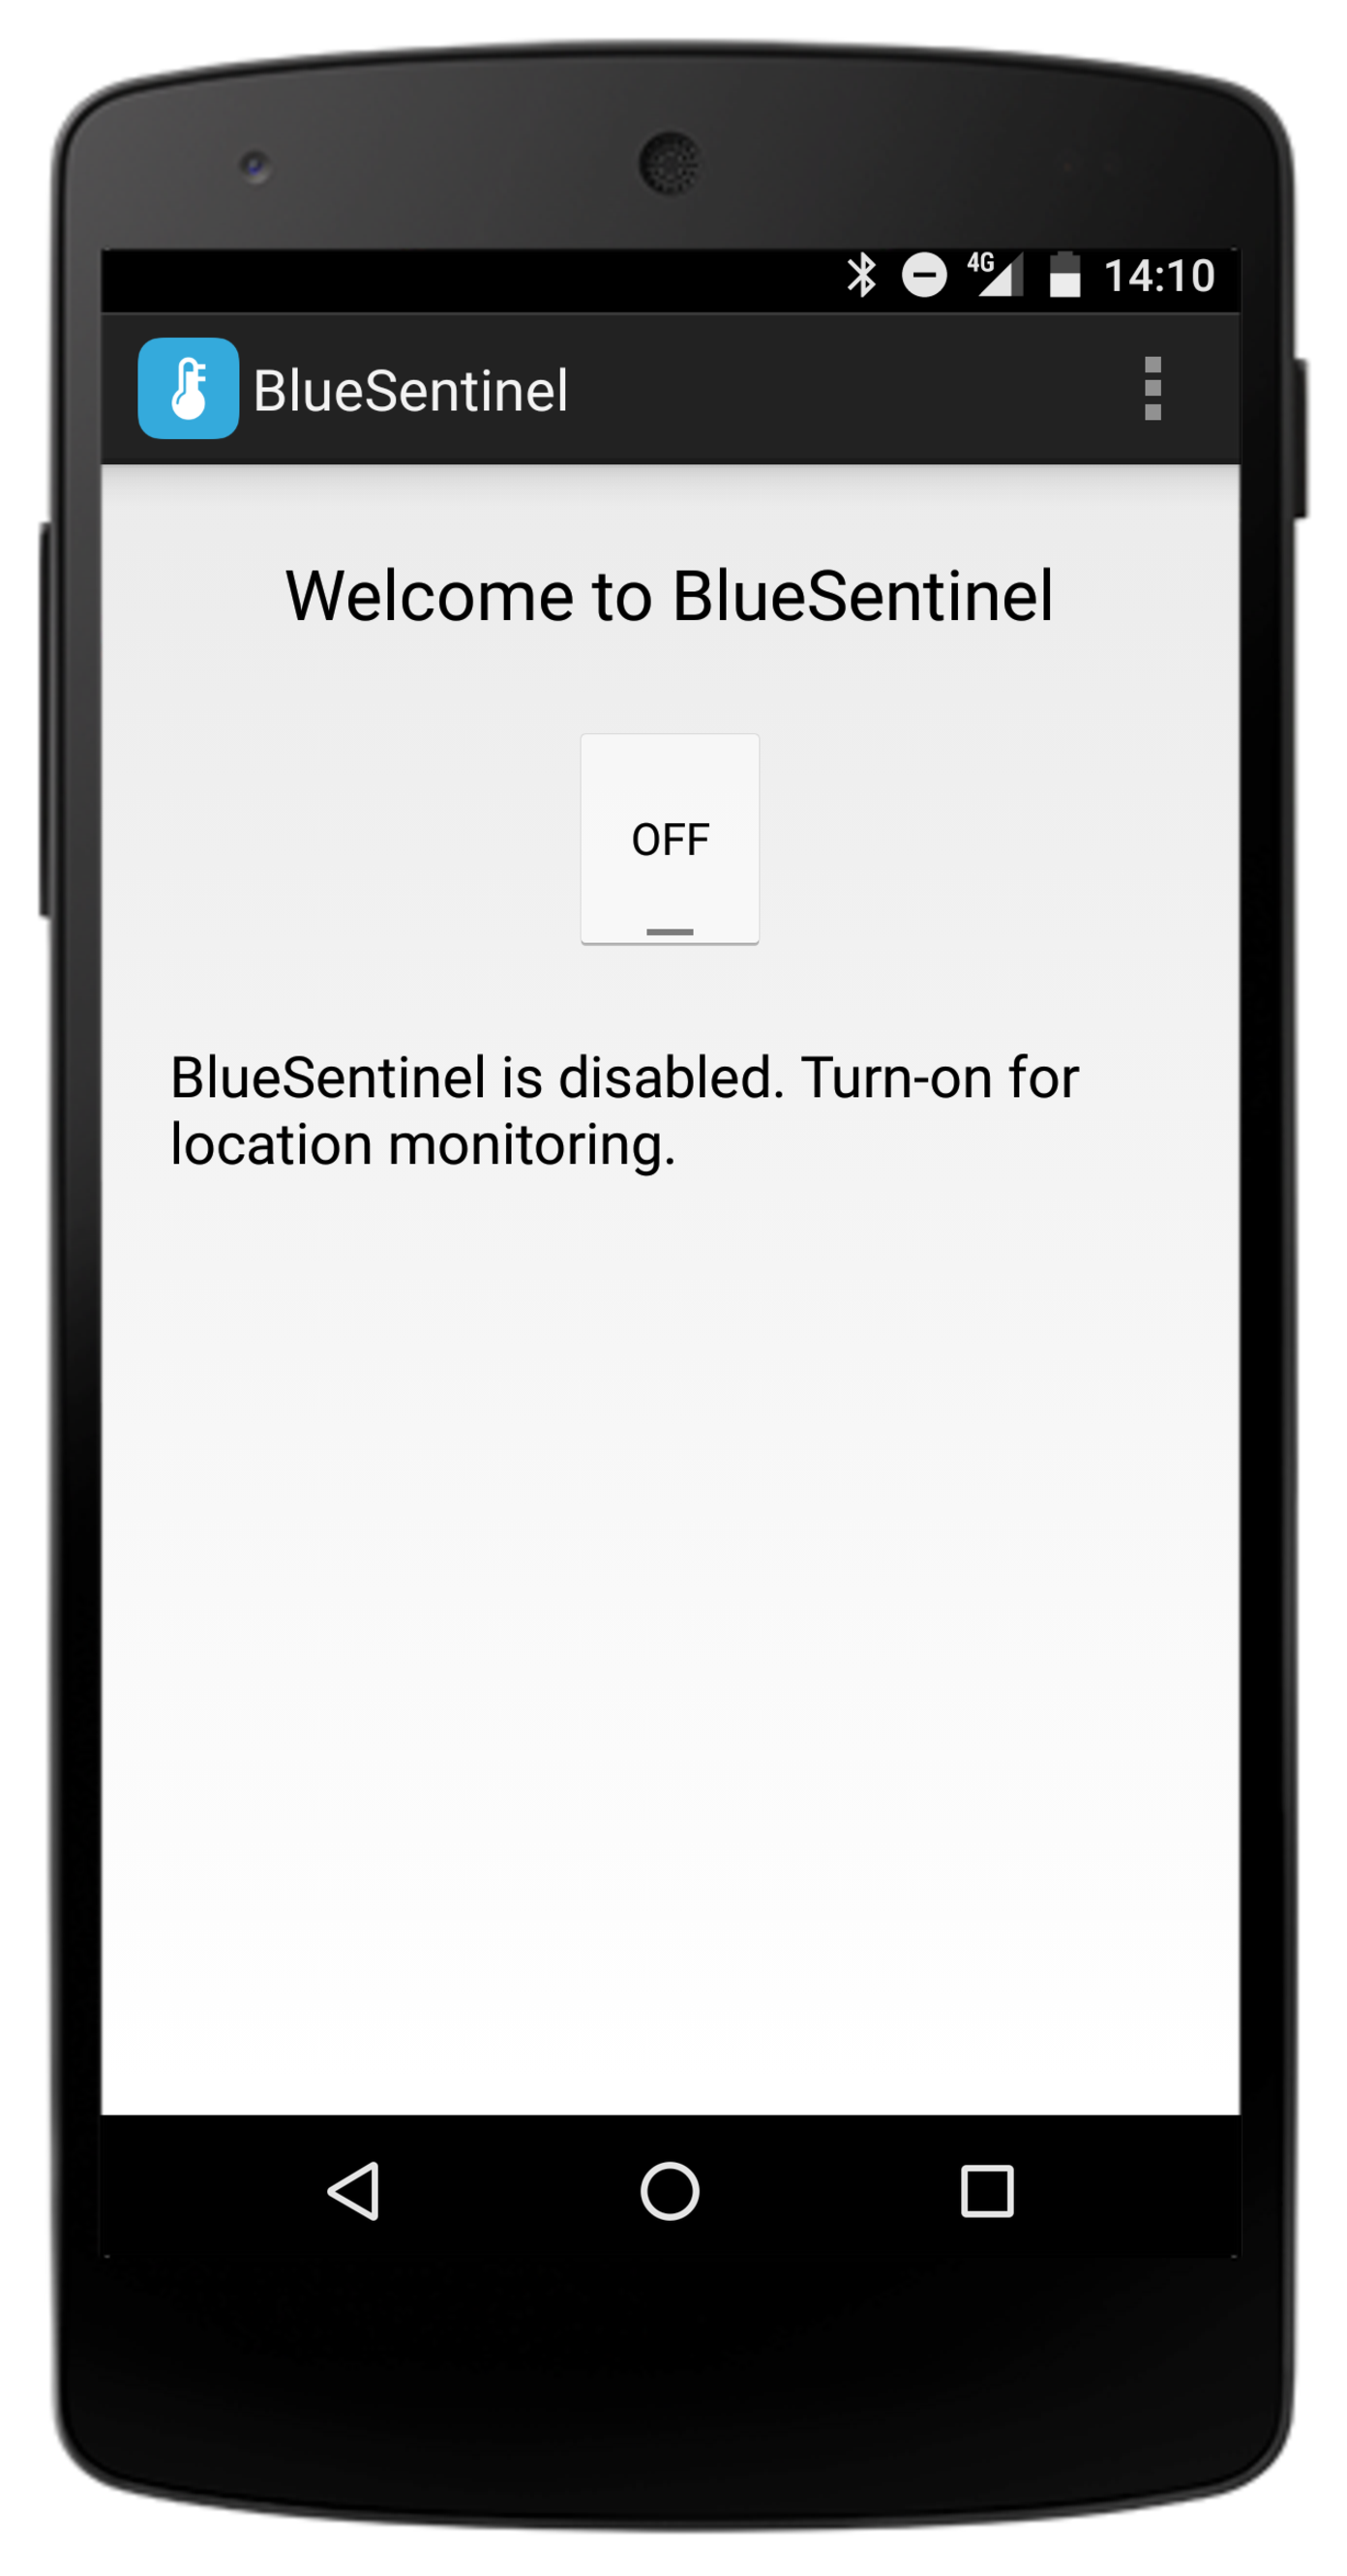
\includegraphics[width=0.8\linewidth]{bsscreen1.pdf}
\endminipage
\minipage{0.50\textwidth}
\center
  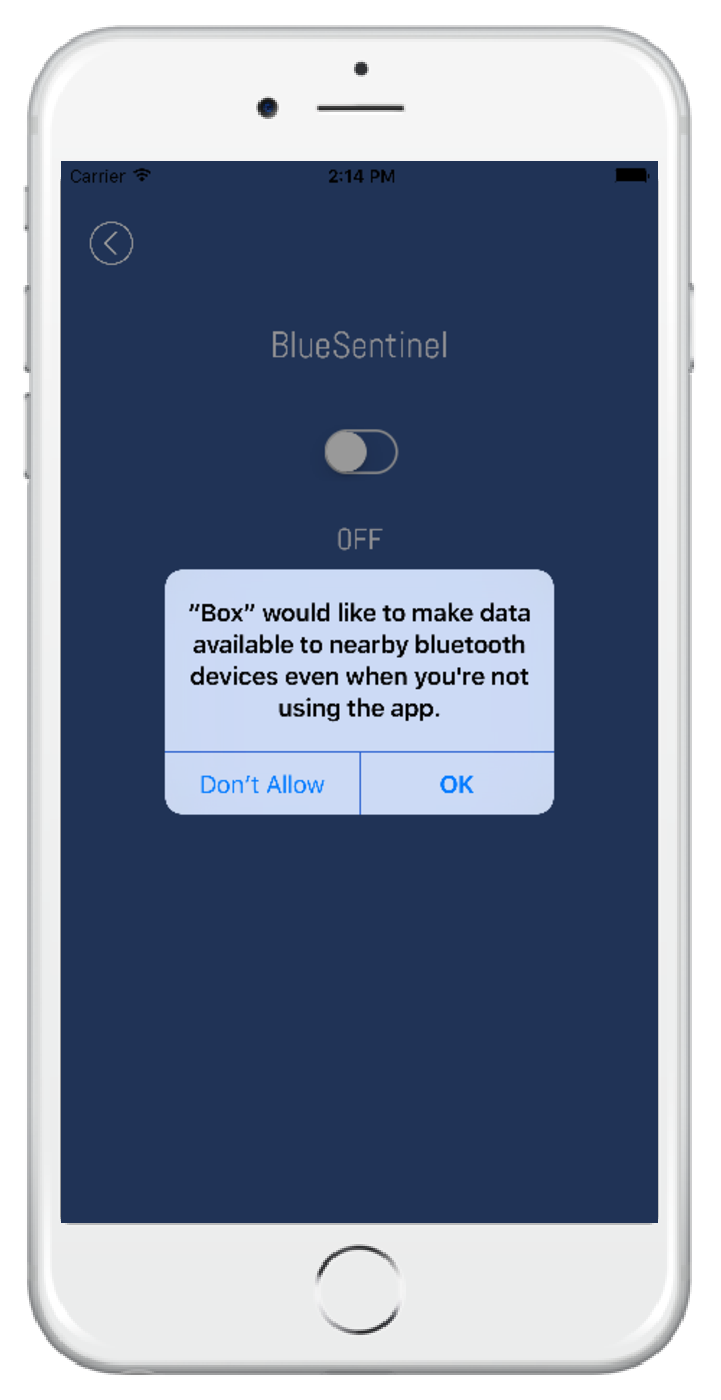
\includegraphics[width=0.8\linewidth]{bsscreen2.pdf}
\endminipage
  \caption{Mobile application developed for Android and iOS devices.}\label{fig:bsscreen}
\end{figure*}

\section{Mobile Application}
\label{sec:app}
A mobile application for both Android and iOS devices has been developed for BlueSentinel users and released on the respective store \cite{NECSTboxAndroid, NECSTboxIos} (Figure \ref{fig:bsscreen}).

The application manages users registrations to the system, asking for e-mail, username and password. Registration has been set up as mandatory; in this way the system is enabled for user identification, but also to build historical data and occupancy probability profiles per single occupant.\\
For each registered user, the system generates an identification string of 10 characters (for example \verb|userId=tslJp2hnqf|). This identifier will be used for both database key and advertisement UUID (Universally Unique IDentifier).

\lstset{
  basicstyle=\ttfamily\footnotesize,
  language=Java,
  columns=fullflexible,
  keepspaces=true,
}

The BlueSentinel menu let the user manage the Bluetooth functionality. Here BLE advertisement can be turn on and off.
In the Android environment BLE advertisement in background is supported by simply implementing the \verb|BluetoothLeAdvertiser| class in an Android Service. The essential code for the advertisement is reported in listing \ref{lst:androidAdv}.

\begin{minipage}{\linewidth}
\begin{lstlisting}[caption={BLE advertising of user identification for Android devices.}, label={lst:androidAdv}]
    private void startAdvertising() {
    		// Retrieve user identification string from database
        String userId = ParseUser.getCurrentUser().getObjectId();
        ParcelUuid pUuid = new ParcelUuid(UUID.fromString(UuidFromString("BLSNTL" + userId)));

        bleAdvertiser = BluetoothAdapter.getDefaultAdapter().getBluetoothLeAdvertiser();
        AdvertiseSettings settings = new AdvertiseSettings.Builder()
        				// Balanced transmission frequency
                .setAdvertiseMode(AdvertiseSettings.MODE_BALANCED)
                // High transmission power
                .setTxPowerLevel(AdvertiseSettings.TX_POWER_HIGH)
                // No time limit
                .setTimeout(0)
                .setConnectable(false)

        AdvertiseData data = new AdvertiseData.Builder()
        		.addServiceUuid(pUuid)
                .setIncludeDeviceName(false)
        bleAdvertiser.startAdvertising(settings, data, advCallback);
    }
\end{lstlisting}
\end{minipage}

User identification string is retrieved from database, converted into a 128-bit UUID and added to the advertisement data. An identification token ("\verb|BLSNTL|") is used as prefix in the UUID; the purpose of the prefix is to discriminate BlueSentinel UUIDs from packets advertised by unrelated devices in the environment, such as BLE headphones or wristbands. Considering 6 chars for the prefix, and the 10 chars of the id, the string of 16 characters can be contained in the 16 bytes of the UUID using the 8-bit ASCII encoding. The resulting Bluetooth packet is represented in figure \ref{fig:payload-detail}.

\begin{figure}[h!tb]
\centering
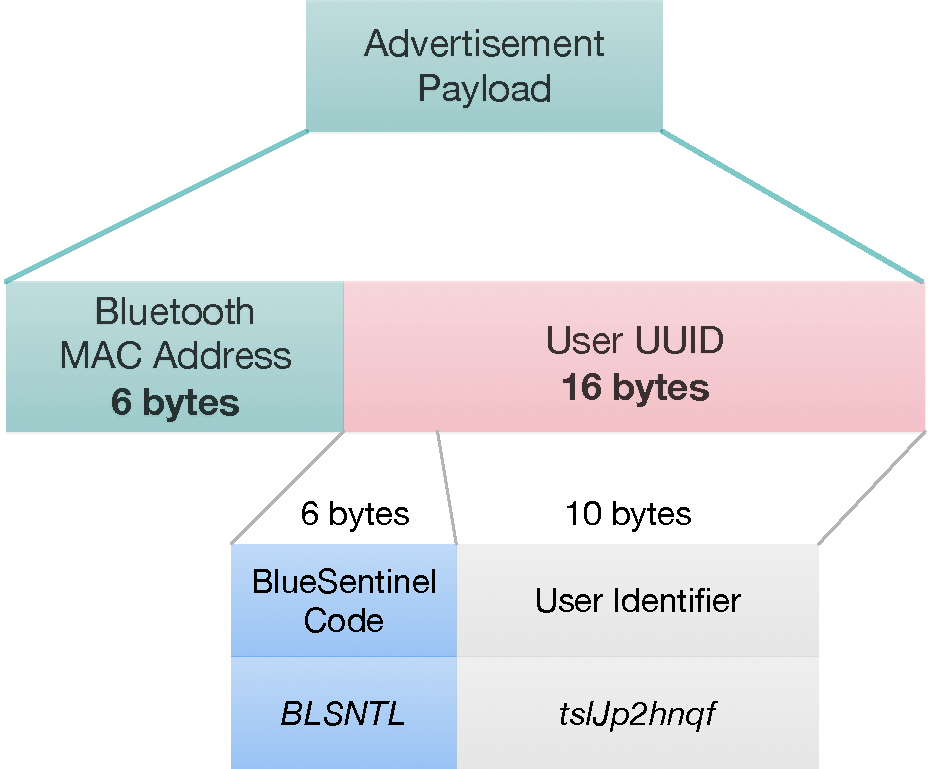
\includegraphics[width=0.6\linewidth]{payload-detail.pdf}
\caption[Detail of the BLE packet advertised by each BlueSentinel user.]{Detail of the BLE packet advertised by each BlueSentinel user.}
\label{fig:payload-detail}
\end{figure}

\medskip
In iOS SDK beacon functionalities are implemented in the CoreLocation framework, which supports all that it is needed to replicate beacons through an iDevice.
However, the CoreLocation framework places many limits on how it can be used in the background.\\
The application has been implemented exploiting the CoreBluetooth framework, that has much greater background support of iOS apps. With CoreBluetooth, it's possible to broadcast as a peripheral and detect as a central while in the background. The Objective-C code that performs the advertising is similar to the equivalent \ref{lst:androidAdv}, where the \verb|CBPeripheralManager| take the place of the \verb|BluetoothLeAdvertiser| class.


\medskip
In addition to the application for building users, a separate application has been developed for the building administrator in order to perform the training of the classification algorithm. The training requires the creation of a label for each building zone; then the administrator needs to travel across each building zone, stop for some seconds and declare the correct room label. Meanwhile, on the server side, the training phase creates a set of RSS samples, each one of them labeled with the corresponding ground truth location.

\section{Wireless Sensor Network}
\label{sec:wsn}
On the building side, the system requires a set of hardware nodes deployed in the indoor environment able to collect BLE packets and contact a centralized server. The node prototype has been developed using Raspberry Pi 3, one of the most cheapest board that supports all the necessary connections. In particular, the mentioned single-board computer provide a BLE module, and both WiFi and Ethernet for Internet connections.

\begin{figure}[h!tb]
\centering
\includegraphics[width=0.6\linewidth]{raspberry.png}
\caption[Prototype of BlueSentinel sensor nodes using Raspberry Pi 3 boards.]{Prototype of BlueSentinel sensor nodes using Raspberry Pi 3 boards.}
\label{fig:raspberry}
\end{figure}

Raspberry boards support a Debian-based Linux distribution, that has been used for the BlueSentinel nodes. The routine that runs continuously on each board has been written in Python, since the most supported library to manage BLE connections is provided for that language. The routine is divided in three concurrent threads:

\begin{itemize}
\item \textbf{BLE scan}: a thread is in charge of collecting every single BLE advertising signal coming from BlueSentinel users. Received packets are first filtered, searching for the BlueSentinel token inside the packet payload. All the unidentified signals are discarded, while the useful packets are stored in a queue. In particular, for each BlueSentinel packet, the thread stores the user Id, the corresponding Received Signal Strength (RSS) expressed in dBm (Decibel-milliwatt), and a timestamp representing the receiving instant.
\item \textbf{Filtering}: Like any other indoor radio-frequency signal, BLE advertisement suffer from signal fluctuations due to multipath fading. This cause a signal to fluctuate over time even if the transmitter is stationary at a fixed distance from the receiver. To reduce the error caused by fluctuations a low-pass filter is applied to the signal received by each user. The filter implemented is the Exponentially Weighted Moving Average (EWMA) that applies weighting factors to the RSS which decrease exponentially over time. Since any filter applied to smooth the signal will always introduce a delay, the EWMA filter has been selected to prioritize more recent RSS samples. The value $V_t$ is computed at time instant $t$ with the following equation:

\begin{equation}\label{eq:filter}
V_t = \alpha \cdot RSS_t + (1 - \alpha) \cdot RSS_{t-1}
\end{equation}

The weighting for each older datum decreases exponentially, never reaching zero. The $\alpha$ coefficient has been fixed to 0.85.
\item \textbf{Data push}: the third thread is is in charge of pushing RSS values periodically to the server at regular intervals. In particular, in each cycle and for each user detected, this thread send the user id, the filtered RSS values, and the most recent timestamp within the sliding window of the EWMA filter.
The choice of the timestamp is given by the weighting factor that emphasizes exponentially the more recent sample. The server is contacted with a HTTP request.
After that data is pushed to the server, the thread empty the samples queue, so that new signals coming from BLE scan will be evaluated in a new filtering window.
After some attempts with different intervals, the period has been set to 1.5 seconds.
\end{itemize}

Every nodes has been connected to the building LAN infrastructure and set up to be remotely accessed using SSH. Every relevant operation executed by the mentioned threads has been logged in a file, in order to check 

\section{Back-end}
\label{sec:back-end}
The system back-end has been set up using Parse-Server, an open-source API server based on the Express web application framework. The REST API has been exploited to interact with Parse Server from the mobile applications, sensor nodes, and a web page. The JavaScript SDK provided by Parse Server (called Cloud Code) has been used to manage the creation of database objects and the localization algorithm.\\
The system back-end has been structured to provide the building occupancy information through the REST API to any third party components of the Building Management System able to send HTTP requests.

All the platforms used to develop the back-end and the external components are represented in figure~\ref{fig:platforms}.

\begin{figure}[h!tb]
\centering
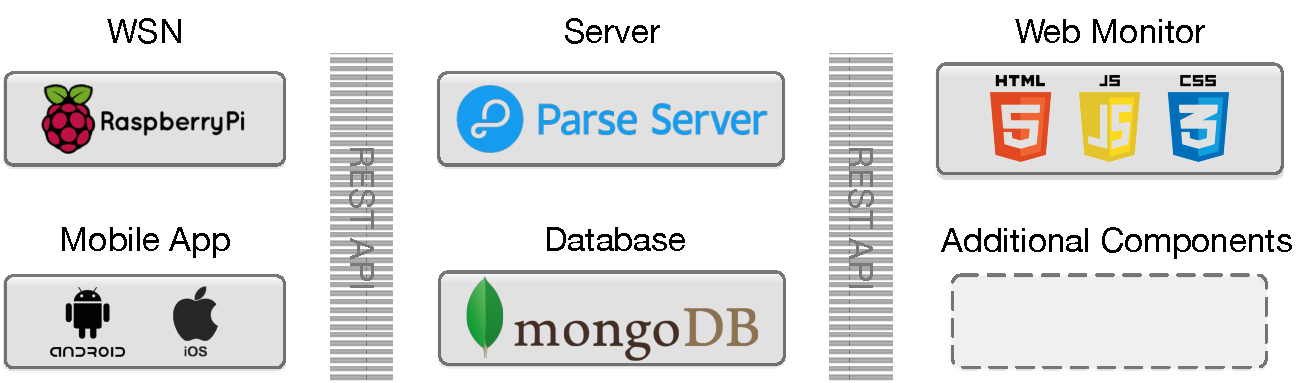
\includegraphics[width=0.9\linewidth]{platforms.pdf}
\caption[Platforms employed for the system back-end and the external components.]{Platforms employed for the system back-end and the external components.}
\label{fig:platforms}
\end{figure}

\subsection{Database}
\label{subsec:db}

The database that supports the system has been implemented using MongoDB. The database contains user objects created during registration. Each zone (or room) of the building has its own instance, created during the training phase by the administrator application. The ReceivedSignal object is created directly by the sensor nodes. It represents the reception of a BLE signal, by a given node. The object is created with the user id founded in the signal, and the received signal strength. The ReceivedSignal data is used by the fingerprinting algorithm to compute each user position. Whenever this happens, the outcome is stored using the UserPosition object.

\begin{table}[h!tb]
\caption[BlueSentinel back-end database.]{BlueSentinel back-end database. Underlined fields represent keys of the table.}
\label{tab:db}
\begin{tabular}{c | c c c c}
%\hline
Table & \multicolumn{4}{c}{Fields} \\
\hline
\multicolumn{1}{c|}{User} & \underline{userId} & email & username & hashedPwd\\
\multicolumn{1}{c|}{Zone} & \underline{zoneId} & floor & maxCapacity & label\\
\multicolumn{1}{c|}{Node} & \underline{nodeId} & zoneId & floor & label\\
\multicolumn{1}{c|}{ReceivedSignal} & \underline{userId} & \underline{nodeId} & RSS & \underline{timestamp}\\
\multicolumn{1}{c|}{UserPosition} & \underline{positionId} & \underline{userId} & RSS & \underline{timestamp}\\
\multicolumn{1}{c|}{TrainingSet} & zoneId & zoneLabel & RSS[~] & timestamp[~]\\
\multicolumn{1}{c|}{TrainingSetDiff} & zoneId & zoneLabel & DiffRSS[~] & timestamp[~]\\
\hline
\end{tabular}
\end{table}


\subsection{Fingerprinting Algorithms}
\label{subsec:algorithms}
The localization algorithm in charge of estimating the position of each detected user has been implemented on the back-end using the JavaScript SDK provided by Parse Server.

The fingerprinting technique is based on a preliminary offline phase in which the building administrator create the training set for the algorithm. More specifically, the training procedure provides the creation of a label for each building zone (For example, \verb|OFFICE_1| or \verb|MEETING_ROOM|). Then the administrator needs to visit each building zone and declare the correct room label. During ground truth collection, the application asks to the administrator to remain stationary if the zone is tiny ($< 15 - 20m^2$) or walk around slowly if the zone is bigger. Meanwhile, on the server side, the RSS samples coming from the admin application are collected and stored in the training set together with the corresponding ground truth location. For each location, the number of vector collected must be at least 4; otherwise the fingerprinting for that location is considered incomplete.

\smallskip
The simplest, or \emph{baseline}, training set schema (represented by the TrainingSet entry in database \ref{tab:db}) is those illustrated in the following example (table \ref{tab:sample-simple}):

\definecolor{blizzardblue}{rgb}{0.67, 0.9, 0.93}
\newcolumntype{a}{>{\columncolor{blizzardblue}}c}

\begin{table}[h!tb]
\caption[Example of RSS samples captured during a training phase.]{Example of RSS samples captured during a training phase (baseline training set). Blue cells represent classification features.}
\label{tab:sample-simple}
\begin{center}
  \begin{tabular}{ | c | a | a | a | a | a |}
    \hline
    zoneLabel & zoneID & RSS1 & RSS2 & RSS3 & RSS4\\ \hline
    COFFEE ROOM & \verb|WTbiGlRdxu| & -60 & -81 & -85 & -95\\
    COFFEE ROOM & \verb|WTbiGlRdxu| & -62 & -80 & -86 & -89\\
    COFFEE ROOM & \verb|WTbiGlRdxu| & -70 & -82 & -91 & -96\\
    COFFEE ROOM & \verb|WTbiGlRdxu| & -63 & -81 & -87 & -93\\
    \hline
  \end{tabular}
\end{center}
\end{table}

Using this schema, the zone identifier and the RSS values represent the features of the classification algorithm.
The training samples reported above have been collected with the configuration depicted in figure \ref{fig:necst-sketch}.

\begin{figure}[h!tb]
\centering
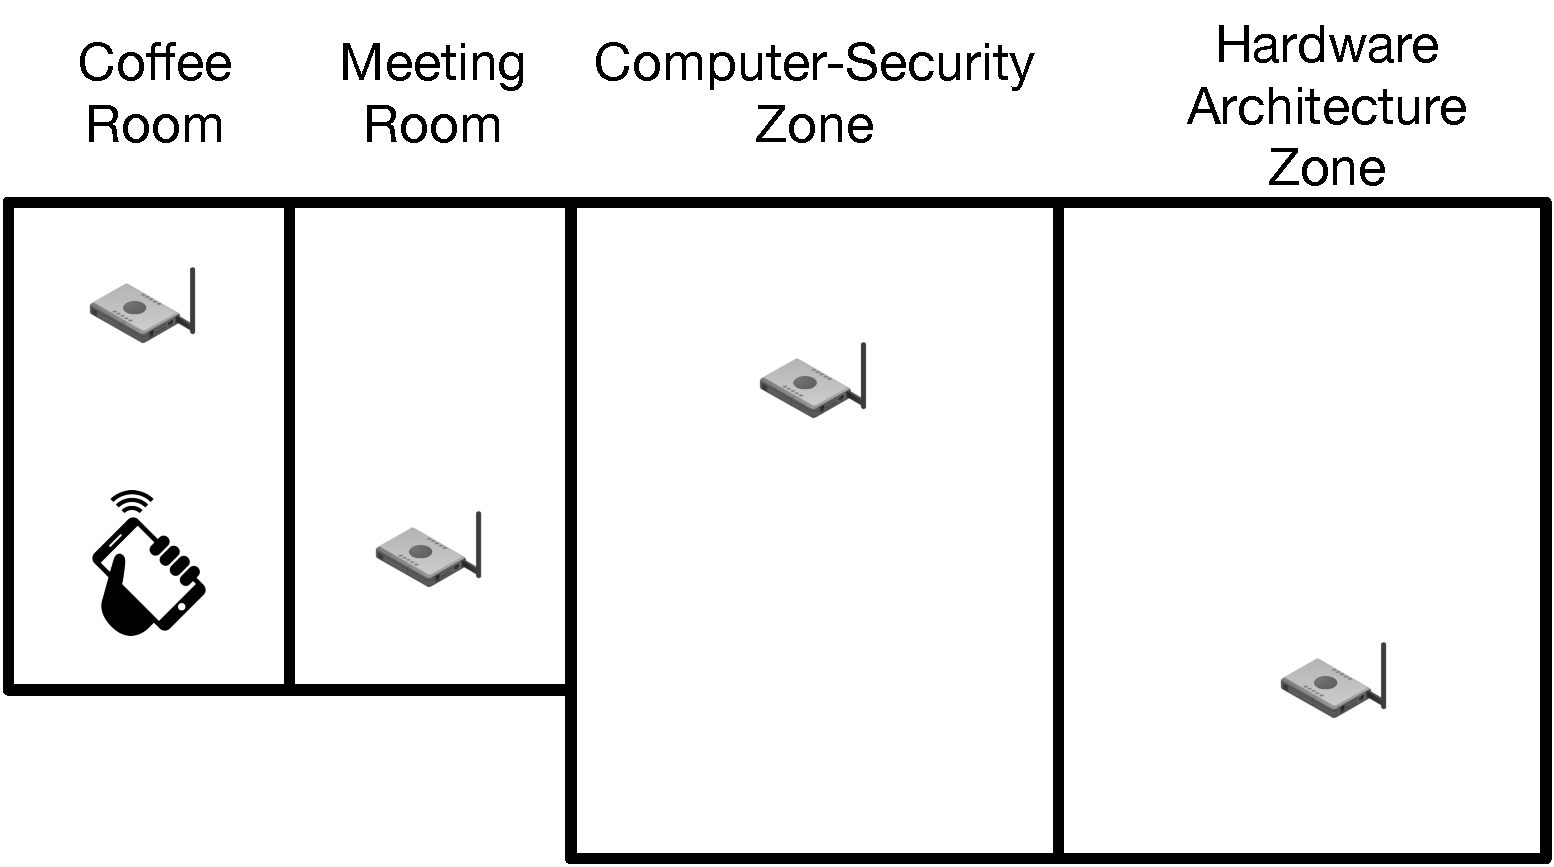
\includegraphics[width=0.8\linewidth]{necst-sketch.pdf}
\caption[Configuration of the system during collection of samples reported in table \ref{tab:sample-simple}.]{Configuration of the system during collection of samples reported in table \ref{tab:sample-simple}.}
\label{fig:necst-sketch}
\end{figure}


Observing the configuration, and thinking on what is the aim of the training phase, a critical issue raises up. The features of the training set are strictly dependent on the particular mobile device where the learning procedure is executed. More specifically, the system will store batches of RSS values that depend not only on the current position, but also on the transmission power of the onboard BLE antenna.
The presence of a hardware dependent classification feature makes the system unreliable when the mobile device that need to be localized at runtime is different from the device used for the training procedure.\\
For this reason, a training set that differs from the \textbf{baseline} has been investigated. The classification algorithm has been trained using \textbf{differential} RSS samples, as shown in table \ref{tab:sample-simple}. In order to make the fingerprinting as more as possible independent from the mobile hardware, the algorithm performs classification based on the difference between RSS values captured at the same time from different nodes. 
The purpose of the differential training set is to reduce the correlation of each vector with the transmission power of the training device, while emphasize the proportions of the RSS vector elements.

\begin{table}[h!tb]
\caption[Example of differential RSS values captured during a training phase.]{Example of differential RSS values captured during a training phase. Blue cells represents classification features. DiffXY represents the difference between the signal strength received at node X and those received by node Y.}
\label{tab:sample-diff}
\begin{center}
\newcolumntype{Y}{>{\centering\arraybackslash}X}
\setlength{\tabcolsep}{.35em}
  \begin{tabularx}{\textwidth}{ | Y | a | a | a | a | a | a | a |}
    \hline
    zoneLabel & zoneID & Diff12 & Diff13 & Diff14 & Diff23 & Diff24 & Diff34\\ \hline
    COFFEE ROOM & \verb|WTbiGlRdxu| & 21 & 25 & 35 & 4 & 14 & 10\\
    COFFEE ROOM & \verb|WTbiGlRdxu| & 18 & 24 & 27 & 6 & 9 & 3\\
    COFFEE ROOM & \verb|WTbiGlRdxu| & 12 & 21 & 26 & 9 & 14 & 5\\
    COFFEE ROOM & \verb|WTbiGlRdxu| & 12 & 21 & 26 & 9 & 14 & 5\\
    \hline
  \end{tabularx}
\end{center}
\end{table}

The training set has been used to train the following classification algorithms.

\subsection{K Nearest Neighbor}
\label{subsec:knn}
For the KNN algorithm, each vector of the training set is virtually positioned in a D-dimensional graph, where D is the dimension of the vector. Since in our testbed there have been employed 4 sensor nodes, the graph has dimension 4 for the baseline training set, and dimension 6 for the differential set.

At run time, the algorithm builds the RSS vector using the user ID and the timestamps of the samples that fall within a short sliding window (1 - 2 seconds). This guarantees that each sample of the vector comes from the same location in the building, since the user can't change position a short window of time.
Whenever a new unlabeled vector is constructed, the algorithm put the element on the virtual graph. At this point, a set of K training points that are the K closest points to the runtime point are selected. From the K labeled observations, a majority vote determines the position label of the runtime sample. The implemented algorithm selects $K=5$ training observations.
The distance between two points $a$ and $b$ (where for instance $a$ is labeled and $b$ is unlabeled) is computed using the Euclidean distance ($E$ for the baseline while $E'$ for the differential case):

\begin{equation}\label{eq:E-baseline}
E(a,b)=\sqrt{(rss_{a,1} - rss_{b,1})^2 + ... + (rss_{a,k} - rss_{b,k})^2}
\end{equation}
\begin{equation}\label{eq:E-differential}
E'(a,b)=\sqrt{(diff_{a,12} - diff_{b,12})^2 + ... + (diff_{a,jk} - diff_{b,jk})^2}
\end{equation}

In equation \ref{eq:E-baseline}, $rss_{a,1}$ represents the RSS value captured by node 1 and stored in the training vector $a$. In equation \ref{eq:E-differential}, $Diff_{a,12}$ represents the difference between training RSS sample of node 1 and node 2, and stored in the training vector $a$.

\medskip
The implemented algorithm computes the distance $E(a,b)$ for every vector $a$ belonging to the training set, sorts in increasing order the resulting list of distances and select the firsts 5 elements for the majority vote. Defining $N$ as the dimension of the training set, and $d$ the dimension of each sample the resulting time complexity to estimate the position each time is $O(dN + NlogN)$.

%TODO: parlare dei dati mancanti

\subsection{Decision Trees}
\label{subsec:trees}
For Decision Trees algorithm, each (baseline) RSS vector has been normalized using the Min-Max scaling. Each normalized element $\widetilde{rss_i}$ has been computing using the following equation (\ref{eq:norm}), where $rss_i$ is the raw sample, while $\vec{rss}$ is the entire RSS training set:

\begin{equation}\label{eq:norm}
\widetilde{rss_i} = \frac{rss_i - min(\vec{rss})}{max(\vec{rss}) - min(\vec{rss})}
\end{equation}

For each feature, a splitting attribute $s$ has been defined as the mean value from the entire data set of that feature. The splitting attribute is used to identify a runtime value as low if it is lower than $s$, or high if it is equal or higher than $s$.

Successively, in order to build a valid decisional tree, the following procedure has been applied to each feature and for each classification in turn. Consider the feature $\widetilde{rss_1}$ and the classification "COFFEE ROOM". The feature has two possible values: low and high. Some of the training samples are low, and we call this set of samples $LOW$. Other samples have been identified as high, and we define this set as $HIGH$. for each one of the two sets, an histogram is built over the classification label "COFFEE ROOM", as shown in figure \ref{fig:tree}.

\begin{figure}[h!tb]
\centering
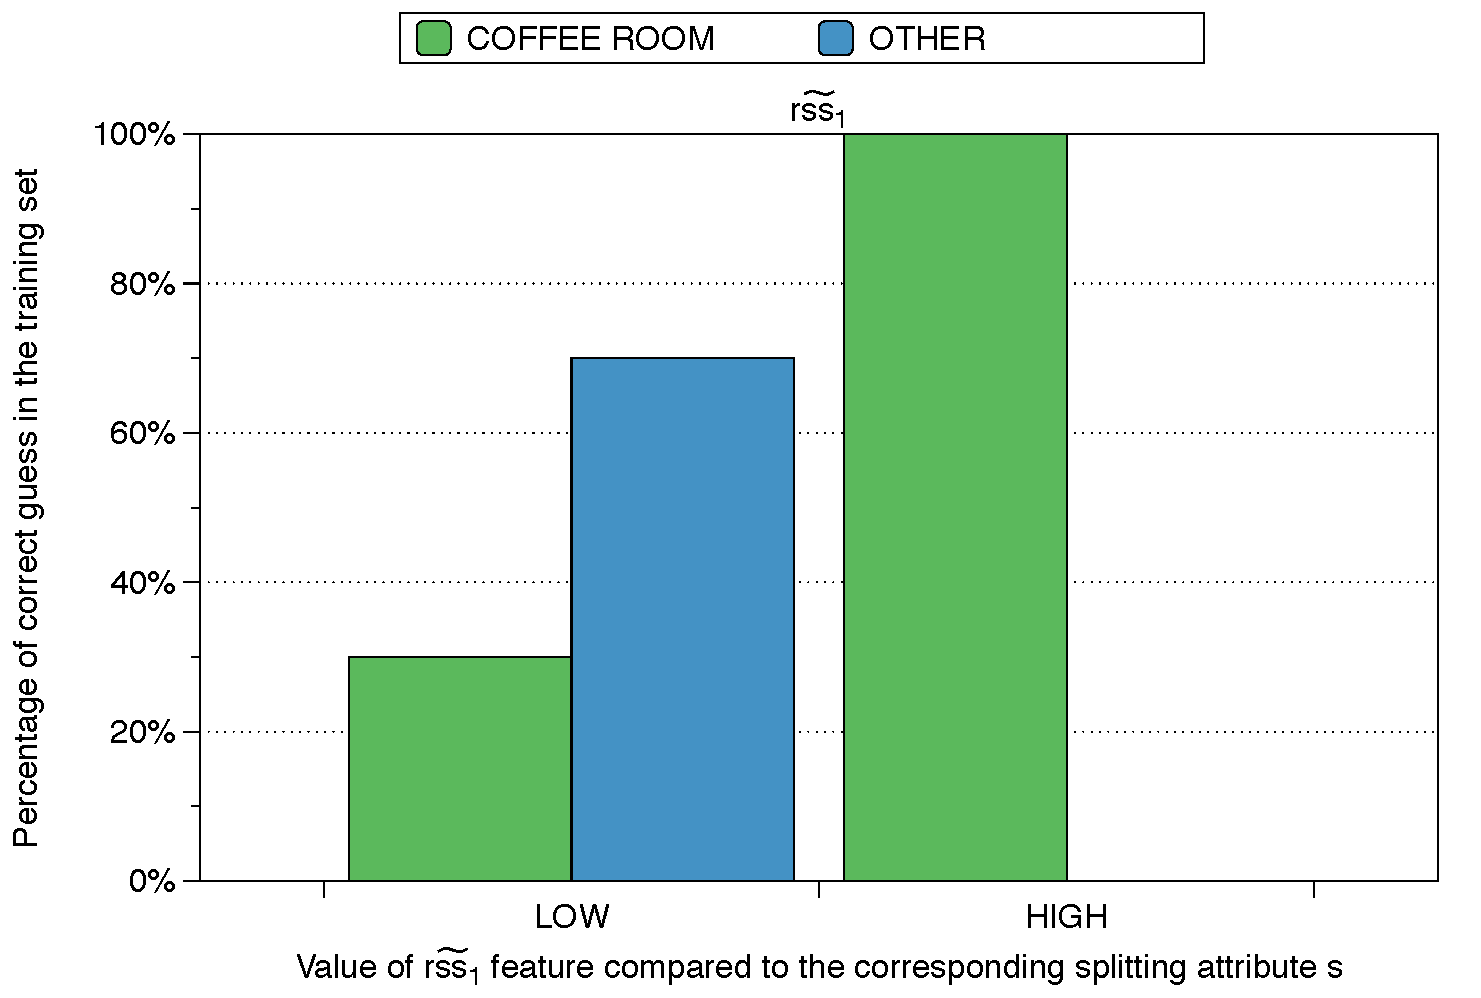
\includegraphics[width=\linewidth]{tree.pdf}
\caption[Example of data normalization using Min-Max scaling.]{Example of data normalization using Min-Max scaling. The histogram shows frequency for each one of the \emph{bucket}.}
\label{fig:tree}
\end{figure}

 Now it's possible to check how much the "COFFEE ROOM" classification is correct if the guess is made exclusively on the $\widetilde{rss_1}$ feature.
In the HIGH set the classification performs 100\% correctly. In the LOW set the classification performs 70\% of them correctly, while 30\% wrong. So overall you would classify 17 out of 20 correctly (85\%). Thus, we can say that the \emph{score} of the $\widetilde{rss_1}$ feature is 85\%. 

The mentioned score is used to sort all the features from the highest to the lowest score, and the order is used to build the decision tree, applying each time the subsequent feature.

\smallskip
The procedure explained however, provide the binary classification that localizes the user inside coffee room or outside coffee room. To obtain the multi-class classification that identify the correct building zone, it is possible to apply the binary classifier repeatedly and combine the results to get the multi-class classification.

% SPLITTO RANGE IN PIU DI DUE INTERVALLI. CANCELLARE SE ALBERI NON BINARI è SBAGLIATO
% After normalization, each RSS vector is composed by values that can range from \numrange{0}{1}. The range has been dived in 5 \emph{buckets} (0.0-0.2, 0.2-0.4, 0.4-0.6, 0.6-0.8, 0.8-1.0) as shown by the example in figure \ref{fig:norm}:

% \begin{figure}[h!tb]
% \centering
% 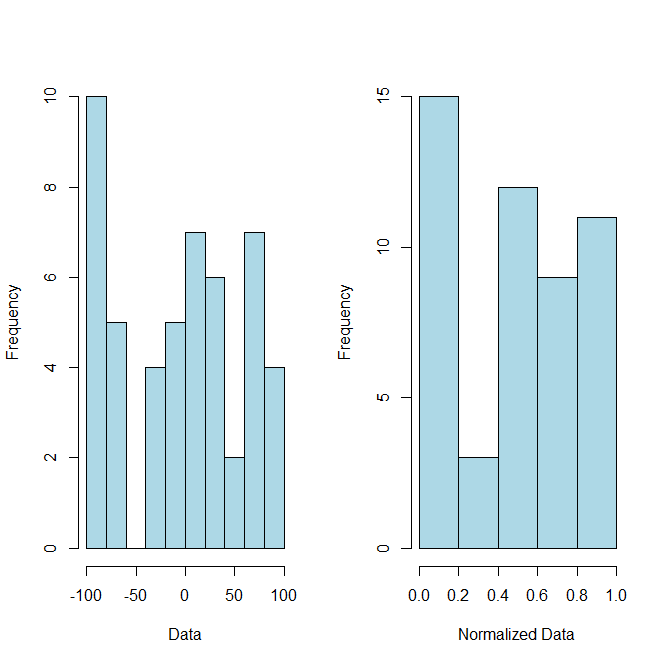
\includegraphics[height=11cm, width=13cm]{norm.png}
% \caption[Example of data normalization using Min-Max scaling.]{Example of data normalization using Min-Max scaling. The histogram shows frequency for each one of the \emph{bucket}.}
% \label{fig:norm}
% \end{figure}
% Successively, in order to build a valid decisional tree, the following procedure has been applied to each feature and for each classification in turn. Consider the feature $\widetilde{rss_1} > 0.8$ and the classification "COFFEE ROOM". The feature has two possible value: no and yes. Some of the training samples have an answer "no", and we call this set of samples $CR$. Other samples have an answer yes, and we define this set as $Y$. for each



\section{Integration with a Thermal Comfort System}
\label{sec:thermosense}

\begin{figure}[h!tb]
\center
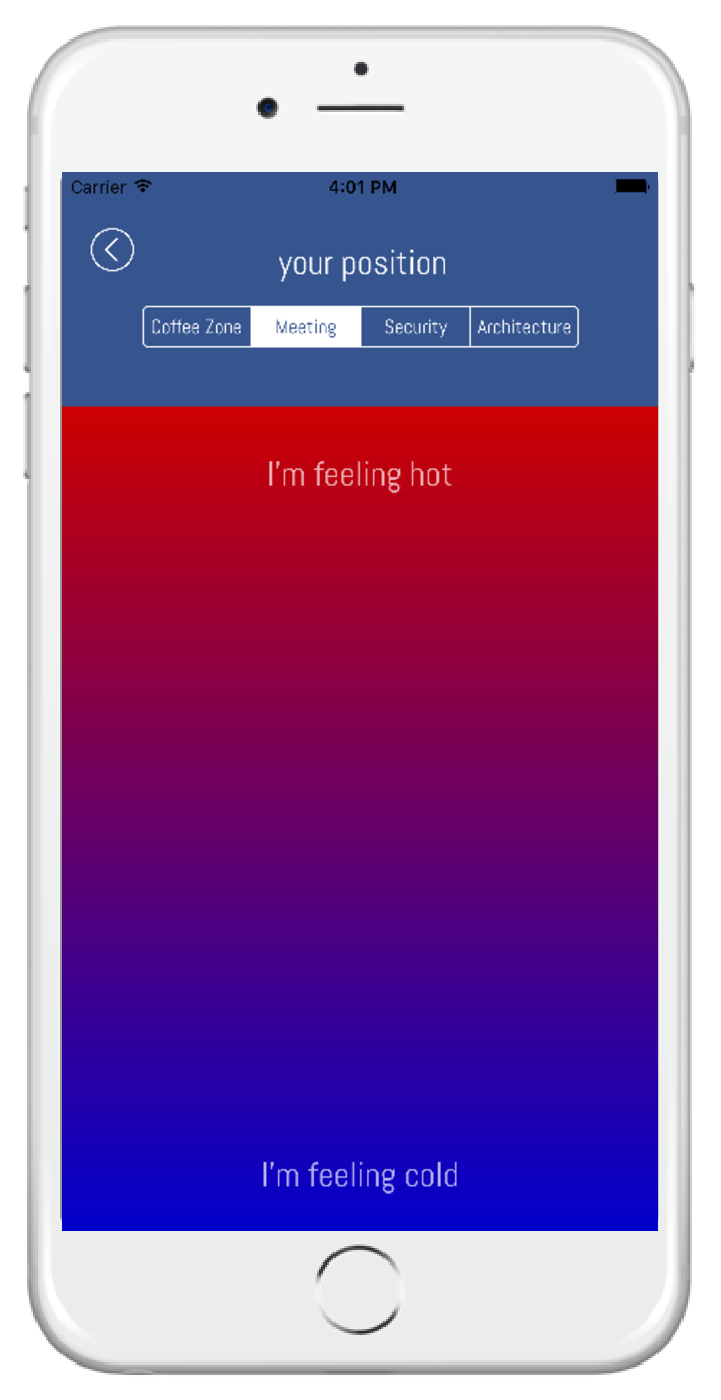
\includegraphics[width=0.3\linewidth]{tsscreenshot.pdf}
\captionof{figure}[ThermoSense user interface that collects thermal complaints from building occupants.]{ThermoSense mobile application user interface.}
\label{fig:thermoUI}
\end{figure}

BlueSentinel has been integrated with \emph{ThermoSense}
\footnote{ThermoSense project: \url{http://box.necst.it/thermosense.html}}, a thermal comfort system developed in our laboratory.\\
The mobile application described in section \ref{sec:app} has been used in conjunction with BlueSentinel and ThermoSense. In particular, while the BlueSentinel module manages all the Bluetooth functionalities, ThermoSense module collects information on the current thermal comfort of the tenants. Users are able to provide a thermal comfort feedback (a complaint) that quantifies the amount of cold or hot perceived through a gradient interface. The feedback information, together with the user position detected by BlueSentinel, is used by ThermoSense to compute the best possible HVAC set point to satisfy the occupants comfort while minimizing the building consumption.
The position information is retrieved by the decisional engine of ThermoSense directly on the backend level. However, any other smart building application developed as a third-party components can retrieve the building occupancy information using the REST interface explained in section \ref{sec:back-end}.


\section{Real-World Deployed System}
\label{sec:lab}

\section{Web-Based Monitoring Dashboard}
\label{sec:webmonitor}
The occupancy information computed by BlueSentinel has been visualized in a web monitoring page. The page shows location data in three forms.\\
First a text table reports the current number of occupants for each zone or room. Together with the occupants number, is available the time instant in which the last user has been seen in the zone.\\
The real-time occupancy is also reported in a heat-map that represents the population distribution inside the indoor environment. The heat-map shows in dark red the more populated zones, while in yellow and white semi-empty or empty rooms.\\
Another chart has been used to visualized the occupancy history of each building zone. Each line represent the number of people in a room as a function of the time.

In all the dashboard elements, users identity has never been showed to guarantee the occupants privacy.

%TODO: spostare o cancellare
% \section{Implementation Decisions}
% \label{sec:decisions}

\section{Limitations}
\label{sec:limitations}
%advertising background for ios. backwards compatibility android. --> detection delays
A first limitation of the proposed approach regards the numerous mobile devices that doesn't support BLE advertising. These can be classified in two categories: devices presenting a version of Bluetooth lower than 4.0 (non BLE), or devices supporting BLE but without a built-in peripheral chipset.\\
For both these two cases, a workaround as been exploited in the BlueSentinel system to provide a backward compatibility to older devices. At this purpose, when the Android application detects the lack of advertising support, it edits the so called Bluetooth friendly-name, i.e. the string that the device provide for pairing with surrounding objects (for example "Andrea's phone"). The friendly name is edited so that it contains the userID and BlueSentinel token introduced in section \ref{sec:app}. In addition, the application edits the Bluetooth discoverability time setting it to infinite.\\
The workaround allows the system to extend the compatibility to older devices; however present some drawbacks. First, the sensor nodes (section \ref{sec:wsn}) showed that using this method the discovery time required to detect the devices is higher compared to BLE advertisement, ranging from 2 to 10 seconds. Second, extending the Bluetooth discoverability of the devices is discouraged since can cause security issues.

\smallskip
Another limitation of the proposed approach relies in the possibility to perform Bluetooth LE advertising on iOS devices when the phone is in background state, i.e. when the screen is off.
The Apple documentation states that all service UUIDs contained in the value of the \verb|AdvertisementDataServiceUUIDsKey| advertisement key are placed in a special “overflow” area; they can be discovered only by an iOS device that is explicitly scanning for them. Nevertheless, the iOS developer community has proven that it's possible to access the advertisement key through a BLE advertisement inquiry performed by the scanning device. Unfortunately, during the development of the BlueSentinel sensor nodes, this particular BLE inquiry has revealed to be unsupported by the current BLE libraries for Raspberry Pi boards. However, moving from the single board computer implementation to a more specific hardware nodes, for example a microcontroller based board, could allow a lower level management of the Bluetooth protocol stack.

\section{Conclusions}
\label{sec:conclusion}

In this chapter, the proposed BLE occupancy monitoring system has been described. First, the feasibility study is reported, explaining also the reasons of the adopted design and the technology employed. Then, the architecture of the system has been illustrated, passing through application, sensing and back-end layers. On the application side, has been discussed the potentiality and limitations of the BLE signal advertisement of recent smartphones, one of the key functionalities exploited in our system. Successively, at sensors level, have been discussed the methods of synchronization and signal filtering implemented. For the back-end side, are reported the database employed for the system, and the different classification methods employed for users localization. In addition will be also illustrated how the occupancy information has being visualized in a web application.

the key contribution of the proposed system are:
\begin{enumerate*}[label={\textbf{(\arabic*)}}]
\item extremely low battery consumption of the mobile application that allows the system to run continuously for many hours;
\item the occupancy detection in real-time;
\item an approach that is non-intrusive from the user point of view;
\item simplified installation and training assisted by a mobile application for building administrator.
\end{enumerate*}
%
% -----------------------------END------------------------------------- %
%
% ------------------------------------------------------------------------ %
% !TEX encoding = UTF-8 Unicode
% !TEX TS-program = pdflatex
% !TEX root = ../Tesi.tex
% !TEX spellcheck = it-IT
% ------------------------------------------------------------------------ %
%
% ------------------------------------------------------------------------ %
% 	CAD Deployment

\chapter[CAD Deployment for Indoor WSNs]{Towards Smart Building Design Automation: CAD Deployment for Indoor WSNs}
\label{cap:cad}


\section{Introduction}
\label{sec:CADintro}
As described in chapter \ref{cap:soa}, over the last years many smart buildings applications have been subject of intense research.
Smart environments usually rely on several hardware nodes equipped with sensors, actuators and communication functionalities.
A clear example is the occupancy monitoring system presented in chapter \ref{cap:bluesentinel}, but the same applies for different applications like indoor localization or safety systems.\\
The high level of heterogeneity and the lack of standardization across technologies make design of such environments a very challenging task, as each installation has to be designed manually and performed ad-hoc for the specific building.
On the other hand, many different systems show common characteristics, like the strict dependency with the building floor plan, also sharing similar requirements such as a nodes allocation that provides sensing coverage and nodes connectivity.

The work explained in this chapter consists in a CAD application for the design of smart building systems based on the installation of hardware nodes across the indoor space. The tool provides a site-specific algorithm for cost-effective deployment of wireless localization systems, with the aim to maximize the localization accuracy.

%Experimental results from real-world environment show that the proposed site-specific model can improve the positioning accuracy of general models from the \mbox{state-of-the-art}.
The tool, born to assist the installation of the BlueSentinel system, has become general-purpose and extensible through plug-ins allowing to model building systems with different requirements.
The results of this project have been presented at UBICOMP 2016 \cite{Cirigliano2016} and will be published in TCAD (Transactions on Computer-Aided Design of Integrated Circuits and Systems).

\section{The Nodes Deployment Problem}
\label{sec:deploy-problem}

Many smart buildings applications are based on indoor localization techniques, using location information to optimize the environment and provide context-aware services.\\
Indoor localization systems often require the presence of wireless devices such as Access Points (AP), in order to let the user identify its position by means of a mobile device.\\
Most smart building applications have been developed in order to achieve sustainability, reducing energy waste related to energy-consuming appliances like Heating, Ventilation, and Air-Conditioning (HVAC). Some examples are \cite{Erickson2011} and \cite{Balaji2013}. Smart HVAC systems usually rely on a set of ambient sensors able to collect indoor values of temperature and humidity. This allows the control system to build thermal maps of the indoor environment, locate thermal complaint feedbacks coming from the tenants and regulate only the necessary portion of the physical system.\\
Another target feature of complex buildings is safety, characterized by the ability to respond to crisis events limiting damages and victims. These systems are able to detect safety threats, for example from smoke detectors or heat detectors. Also in this scenario, a proper allocation of sensor nodes is essential to detect and locate the threat responsively.

\smallskip
The position of each node strongly affects the performance of the system, since a bad allocation could lead to unmonitored areas.
%encumber: gravare; sinonimi: burden, weigh (pesare figurato).
The number of nodes employed, besides weighting on the installation cost, also burdens the overall energy consumption of the system, a key parameter to consider especially for energy saving systems.\\
The choice of the hardware nodes can get more difficult by the availability on the market of several devices and components that differ in cost, power consumption and maximum range distance.

\smallskip
Although the key role of nodes allocation, many smart building systems proposed in literature don't consider nodes amount and positioning problems in environments that differ from the original testbeds.\\
Without a systematic approach the design space is not well explored, which leads to inefficient solutions.
In this context, the development of tools able to automatize part of the design flow of smart building systems is essential.
In order to find a near-optimal allocation of nodes, the knowledge of the floor plan is required. However, for installations performed on existing buildings, administrators can encounter difficulties in obtaining the floor plan in an easily-interpretable digital format.
%recupero floorplan, posizionamento, costo totale / accuratezza, installazione è costosa, tuning / spostamento è unfeasible

To address these problems, we developed a CAD tool to assist building designers during the design of smart building systems.
The application manages common requirements like the building floor plan specification. We decided to implement a node allocation algorithm for three different indoor localization systems, that searches for  near-optimal 
%aiming to keep low ...
allocations of nodes, from mixed hardware types, with the aim of keeping low the total cost. Due to the high level of heterogeneity and lack of standardization across systems to design, we make the system extensible through plug-ins to let new functionalities being integrated into the system.
The tool\footnote{A video demo of the tool has been published at \url{https://youtu.be/5BnFU9iXXWo}}
is developed within the QCAD environment \cite{Qcad}, an \mbox{open-source} computer-aided drafting application. The key contributions of our work can be summarized in the following:
\begin{itemize}
\item A traditional CAD interface to specify both the physical building floor-plan and the functional components of the smart environment.
\item An algorithm for hardware nodes allocation that provides to designers a near-optimal placement of devices. The algorithm explores combinations of different types of nodes to obtain cost-effective solutions.
\item A site-specific model for wireless indoor localization accuracy optimization that keeps into account the actual structure of the building.
\item The integration of the tool within an \mbox{open-source}\footnote{The source code of the system is \mbox{open-source} and available at \url{https://bitbucket.org/necst/box-smartcad}} application framework able to extend the system by means of JavaScript or C++ plug-ins.
\end{itemize}

\section{Related Work}\label{sec:related}
Building Information Modeling (BIM) is a consolidate process to support building constructions and renovations. BIM softwares, and in particular CAD for buildings such as ArchiCAD~\cite{Archicad}, focus on the generation and management of digital representations of the physical aspects of places. BIM tools can coordinate architectural and structural requirements, for essential tasks such as collision detection~\cite{Zhang2011}. Materials employed for a construction can be represented with extremely high levels of accuracy, thanks to the several libraries developed in many years, resulting in precise cost estimations~\cite{Xu2014}. With the diffusion of integrated smart systems built to increase comfort and efficiency, buildings require the design of aspects that go beyond the mere physical design. The concept of smart environment is becoming more and more concrete with the integration of sensors, actuators and computational elements in buildings, while tools able to model smart and interactive functionalities of modern buildings are currently lacking.

The problem of the allocation of hardware nodes in a given environment can be compared, on first approximation, by the maximal cover location problem (MCLP), i.e. the problem of covering the maximum amount of demand locations with a given number of facilities. Similarly, the location set covering problem (LSCP) consists in finding the minimum set of facilities that covers all available demand locations. Each facility has the same coverage radius \(r\); a demand point is assumed to be covered if it is within distance \(r\) of a facility. Daskin et al. gave a general formulation of the LSCP \cite{Daskin1983} and re-formulated it for network systems and emergency vehicle deployment \cite{Daskin1981}.

The maximum sensing coverage region (MSCR) is a special case of the previous two problems that focuses on the research of an allocation of wireless nodes that guarantees both sensing coverage and network connectivity between nodes~\cite{VinhTranQuang, So2005}. In this scenario the placement need to take care not only of the sensing range, but also of the communication range of each node.
%Questi approcci citati hanno lo svantaggio di considerare le singole locazioni come variabili binarie coperte/scoperte, senza modellizzare le performance complessive del sistema.

\begin{table}
\centering
\def\arraystretch{1}
\label{tab:comparison}
\caption{Comparison between proposed deployment methods and tools for indoor WSN and Access Points based systems.}
\begin{tabulary}{\textwidth}{| L | L | L | L | L |}
    \hline
    \textbf{Deployment} & \textbf{Site Specific vs General Model} & \textbf{Heterogeneous Nodes} & \textbf{Application Integrated} & \textbf{Extensible} \\ \hline
    Zhao et al. \cite{Zhao2008} & General Model & No & Yes & No\\ \hline
    He at al. \cite{He2011} & General Model & No & No & No\\ \hline
    Fang et. al. \cite{Fang2010} & Site Specific Model & No & No & No\\ \hline
    Proposed approach & Site Specific Model & Yes & Yes & Yes\\ \hline

    \end{tabulary}
\end{table}

For what concern the allocation in indoor environments, only minimum literature has been published so far to the best of our knowledge. Zhao et al. in \cite{Zhao2008} proposed an access point (AP) positioning model based on the Differential Evolution algorithm, specific for fingerprinting localization techniques. Their model focuses on increasing the diversity of the received signal array along the indoor locations, and thus improving the positioning accuracy of fingerprinting schemes.
However, the model does not take into account the effect of walls or other obstacles present in the target environment.
%However, the model is not suitable for triangulation and sensing monitoring positioning problems.
%In addition, the model does not take into account the effect of walls, doors and other obstacles.
He at al. in \cite{He2011} made use of a genetic algorithm for APs deployment model, to study the relationship between positioning error and signal space Euclidean distance. Again, the simulation results show that the error can be reduced increasing the Euclidean distance between the RSS (Received Signal Strength) arrays of different locations.
%This has been achieved increasing the number of APs until a certain range, but the results show that ``the more the better'' rule does not necessarily hold.
%Similarly to the previous work, the authors used a simple signal propagation approach and did not consider the attenuation effects of the indoor environment.
Fang et. al. in \cite{Fang2010} proposed a tool for linking the placement of APs and the positioning performance. Their algorithm maximizes signal-to-noise ratio (SNR) i.e. maximizes the signal and minimizes the noise simultaneously. However, the system is developed in a real-world environment, and requires measurements with different access point allocations that can be an expensive and time-consuming task.

A common limitation of many works described previously is the employment of simple and general models which doesn't take into account the actual layout and geometry of the building. The free-space path loss propagation model is often used despite the presence of fixed obstructing objects like walls. Of course, none of the cited works provide a convenient way to specify geometric layout of the indoor environment. This leads the authors to validate models simply using squared or rectangular areas to represent the indoor environment, omitting the relationship between irregular areas and system coverage.
%The result can lead designers in time-consuming maps configuration, and error-prone design phase for the allocation of hardware nodes.
In addition, none of the existing solutions takes in consideration different hardware characteristics and costs of the nodes to be deployed.

\section{The Proposed Application Framework}\label{sec:components}
Our system has been developed on top of the QCAD application framework. The QCAD Application Framework consists of programming libraries and resources that provides CAD specific functionalities. An example of module provided by the QCAD Application framework is the Math module that implements mathematical concepts such as vectors or matrices as well as basic geometrical classes like points, lines and so on. The QCAD Framework has been enhanced with a \emph{SmartBuilding} module that provides some fundamental functionalities for the design of smart building systems. The module include abstract entities like rooms, walls, sockets, sensor nodes and gateways. User interface components are also provided in order to create and edit this entities (\emph{tools}) and to specify parameters (\emph{widgets}). Our module implements a node deployment algorithm for three commons indoor localization systems, that will be discussed later.
The whole application rely on Qt, a framework that covers a lot of generic and low level functionality for desktop applications and not directly related to CAD.
\begin{figure}[h!tb]
\centering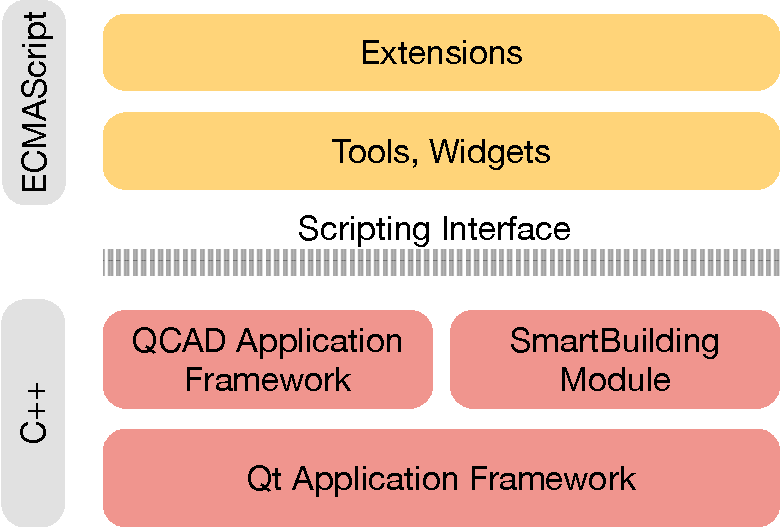
\includegraphics[scale=0.7]{framework.pdf}
\caption[Overview of the CAD application framework stack.]{Overview of the application stack. The script interpreter features standard ECMAScript functionality and on top of that provides additional classes from the Qt API, QCAD API and the \emph{SmartBuilding} module.}
\end{figure}

The QCAD Application Framework offers a very complete and powerful ECMAScript interface. The SmartBuilding module, as well as the QCAD Application Framework, is accessible through that scripting interface. Through the ECMAScript interface developers will be able to extend the whole application in an easy and very efficient way. The choice of a popular script language that is easy to learn enables anyone with previous programming experience to extend the application. Such extensions can for example be CAD related interactive tools like an HVAC layout construction widget, or a temperature sensor nodes deployment algorithm.
%piazzamento sens temp humi, 
%or user interface components (widgets).

In some situations extending QCAD through scripts alone may not be possible. This is mostly the case, if the extension is based on an existing C or C++ library. In that case, it is possible to create a C++ plug-in that wraps the existing library and adds the necessary hooks to access library functionality through the script interface. Such a plug-in will be automatically loaded by QCAD on start up to add functions and classes to the script interface of QCAD. These script extensions can then be used by a script add-ons to make that functionality available as part of the application interface.


\begin{figure}[h!tb]
\centering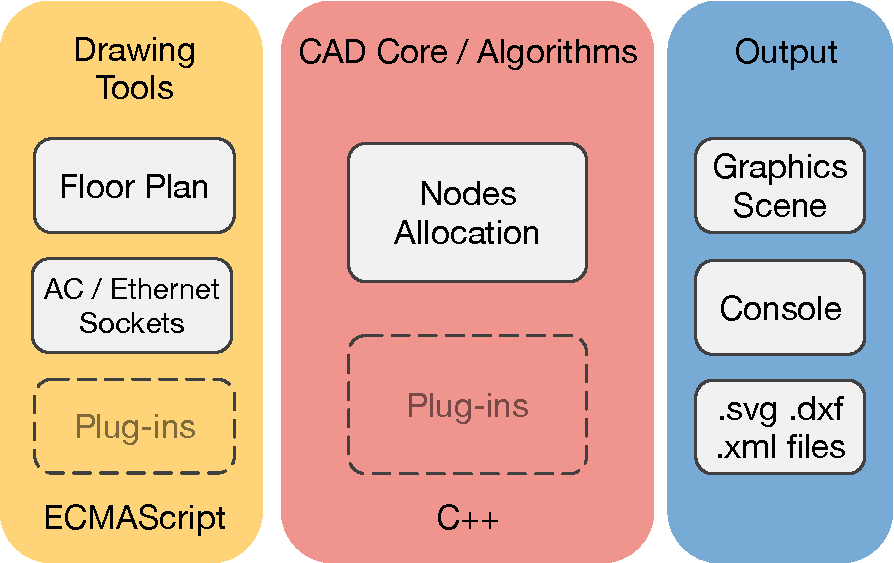
\includegraphics[scale=0.7]{extend.pdf}
\caption[Functional overview of the system components of the CAD application.]{Functional overview of the system components. Drawing tools and algorithms for systems deployment and simulation are extensible through ECMAScript or C++ plug-ins.}
\end{figure}

\begin{figure}
\centering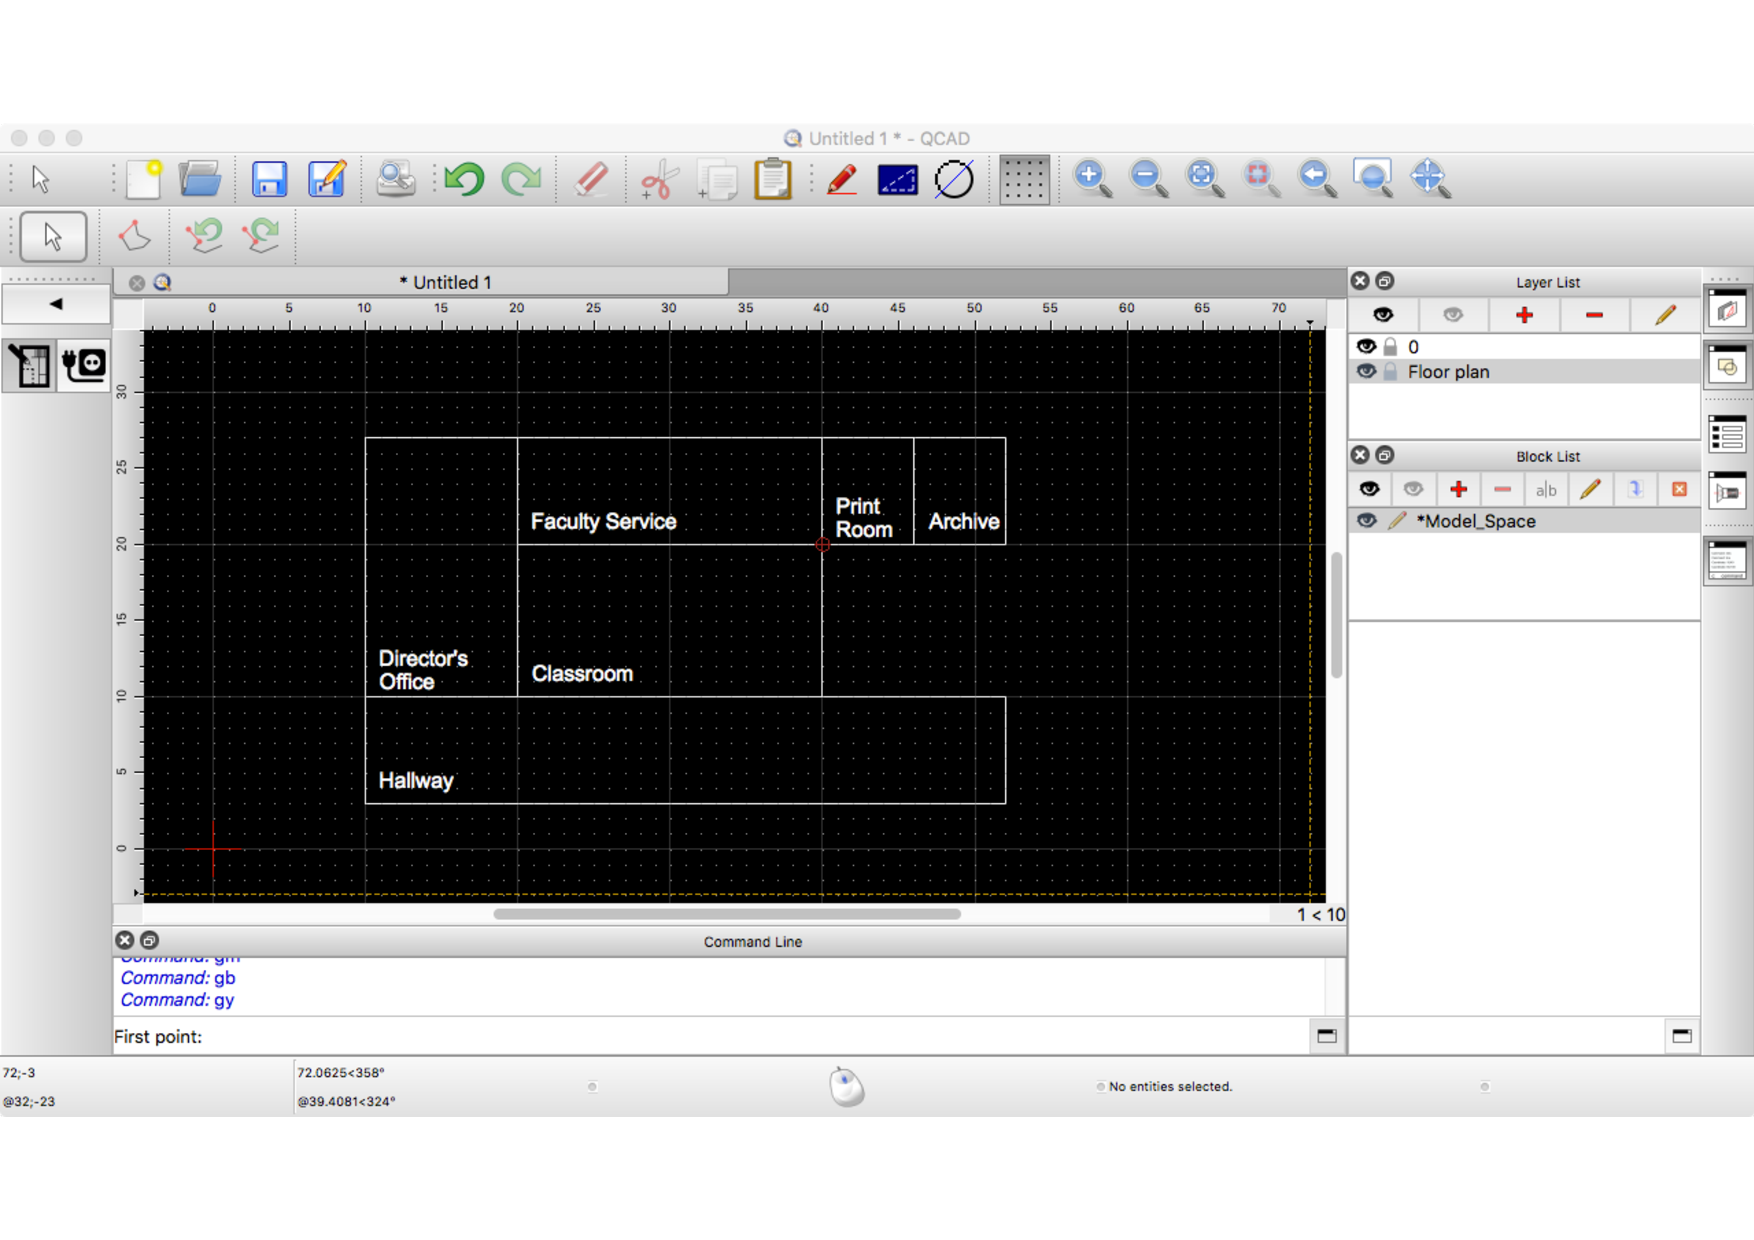
\includegraphics[width=\linewidth]{floorplan2.pdf}
\caption[Graphical interface of the floor-plan design of the CAD tool.]{Floor-plan design tool. User can specify the layout of the rooms and a possible set of candidate sites for the node placement.}
\label{fig:floor}
\end{figure}

\section{Nodes Deployment for Indoor Localization}\label{sec:problem}
Smart environments always rely on a set of hardware nodes able to collect sensing data and communicate through cabled or wireless technologies. The number of nodes employed and the position of each one strongly affect the overall performance of the system as well as the cost of installation.
In our work, indoor localization systems have been taken as the main case study for the nodes allocation, since occupants localization and monitoring is one of the most common requirements of different smart environments.

The way in which the indoor environment must be covered by the nodes depends on the particular technology implemented, however there can be identified three main manners: 
\begin{enumerate}[label={(\arabic*)}]
\item Single Coverage, i.e. to monitor the state of the environment with a single node for each location inside its radius. This includes for example to detect the presence of a mobile device in a proximity region \cite{Andersson2014}, or to detect a RFID tag within the tags reader range \cite{Paul2014}.
\item Trilateration, to compute the position of a mobile device. This technique requires the reception of a wireless signal of at least three reference sensors with well-known positions everywhere within the covered area. We define the term \mbox{$k$-coverage} as the minimum number of sensors (or reference nodes) required in each location by a system. Single coverage systems have \mbox{$k$-coverage} $ = 1$, while for trilateration $k=3$.
\item Fingerprinting, where the number and the strength of the received signals is not fixed, but affect the localization accuracy.
\end{enumerate}
Trilateration and fingerprinting usually exploit wireless technologies as Wi-Fi or Bluetooth to establish a connection between mobile and stationary nodes. Sensing regions can refer to any type of ambient sensors, such as Passive Infrared Sensors (PIR) \cite{Erickson2013}, remote thermal sensors \cite{Beltran2013}, but also proximity based radio transmitters such as RFID tag readers \cite{Zhao2014} and Bluetooth Low Energy transmitters (BLE beacons) \cite{Nacci2015}.
%During the installation phase, the choice of the hardware nodes can get more difficult by the availability on the market of several hardware components that differ in cost, transmission power and maximum range distance.
\section{The Proposed Deployment Tool}\label{sec:plan_tool}
%valutare la possibilità di inserire, oltre che al sensing range, anche il communicatrion range
As we previously said, smart environments always rely on a set of sensor nodes, each one able to communicate through cabled or wireless technologies. Also for outdoor WSNs, a key challenge is how to achieve coverage of the target monitoring space and sufficient network connectivity between sensor nodes. Usually each sensor mote communicates with the rest of the network through technologies like Wi-Fi or Zig-bee. Additional issues for outdoor WSNs are the limited battery life of each node and the power consumption required for packet transmissions. Given the availability in most (also "non-smart") buildings of power outlets, Ethernet sockets and Wi-Fi signal, the mentioned limitations of WSNs can be solved in indoor application making use of the existing infrastructure. Differently from outdoor WSN deployments, where coverage and connectivity are always treated together, our system leaves nodes connectivity optional, focusing on providing the coverage service to the indoor locations.
%Far notare che la connectivity ha senso per single coverage, mentre per trila e fing, dove i nodi sono tx, sensing e communication sono lo stesso range. In realtà non è così! vedi bluesentinel

The design process starts with a drafting phase in which the user specify the building floor plan as a set of rooms. During this phase the designer can restrict the possible sites for nodes allocation, selecting a set of candidate points. This can be useful when the hardware devices require power supply or Ethernet connectivity. The design interface used for both map and candidate sites specification is reported in Figure~\ref{fig:floor}.

In our model, we will refer to \(L\) as the entire set of monitoring locations to be covered, while \(J\) as the set of deployable locations where nodes can be placed. By default, \(L = J\) and nodes can be positioned everywhere but as we said the set \(J\) can be restricted only to specific candidate points.

After the design phase, different parameters are provided by the administrator and used to define a domain in which search for a covering solution. The parameters are:
\begin{itemize}
\item The covering technique (single, trilateration or fingerprinting) that will be used to cover the locations in $L$;
\item A cost \(c_t\) for every type \(t \in T\) of node available on the market (expressed in dollars);
\item A working range \(r_t\) for every type \(t\) of node (expressed in meters);
\item A percentage of covered area required, called $target$ (i.e. the minimum percentage of locations $l \in L$ to be covered by the solution).
\end{itemize}
The system will return to the designer a set $N$ of nodes $n_{jt}$ (possibly with mixed hardware types) and their position on the building map. The outcome will have the lower cost of installation among all the inspected solutions that satisfy the \emph{target} percentage of covered area. Figure~\ref{fig:main} shows an overview of the process explained so far.

\begin{figure}[h!tb]
\centering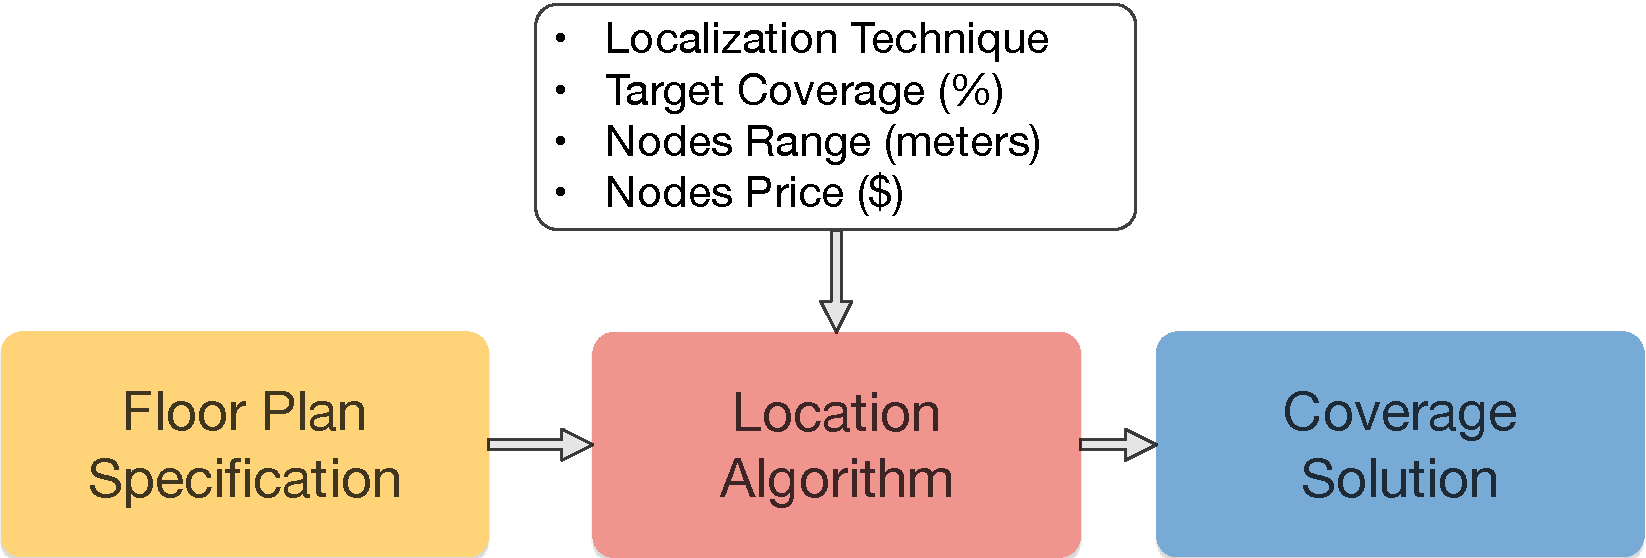
\includegraphics[width=\linewidth]{main.pdf}
\caption[System process of the CAD deployment tool for indoor WSNs.]{System Process. After the design of the floor plan, different parameters are used to define the search for an optimal allocation of nodes.}
\label{fig:main}
\end{figure}


\subsection{Covering Techniques}
\label{subsec:covering}
Our tool provides three different ways to cover the floor-plan space, each one identified by the technique required by the system that will be installed.
\begin{enumerate}[label=\textbf{(\arabic*)}]
\item \textbf{Single coverage}, that guarantees from each position the presence of at least one reachable node. This is used for example to detect the presence of a mobile device in a proximity region. In our model, a location \(l\) of the floor-plan is considered covered if exists at least one working node \(n\) of type \(t\) within a range \(r_t\). An example is shown in Fig.~\ref{fig:coverage}.a.
\item \textbf{Trilateration} is the process of determining the position of a point measuring its distance from three reference nodes, exploiting geometric properties of triangles. Usually, indoor trilateration systems use the strength of the signal received from a node to estimate its distance. In our model, a location \(l\) of the floor-plan is covered for trilateration if there exist at least three working nodes \(n_1, n_2, n_3\), each one no more distant then its corresponding range \(r_t\). A location $l$ served for trilateration is shown in Fig.~\ref{fig:coverage}.b. Although we refer only to trilateration, the same exact result can be used also for triangulation, the technique where angles are measured instead of distances.
\item \textbf{Fingerprinting}: this technique is used to estimate the position of a mobile device based on its received signal strength ($rss$) vector. Each location receives the signal from \(k\) nodes, where \(k\) is not the same for all locations, but depends on how many nodes are reachable from that particular location. Each one of the \(k\) signals reaches the receiving antenna with a given power (or $rss$). For example, the location $l$ shown in Fig.~\ref{fig:coverage}.c perceives $k=2$ signals so that $rss_{l,1} < rss_{l,2}$. We denote as \(rss_{l,n}\) the signal strength received at location \(l\) from a node \(n\). The vector \(\vec{rss_l} = [rss_{l,1}, ..., rss_{l,k}]\) of the \(k\) signals received at run-time in location $l$ is compared with a dataset of vectors, each one pre-labelled with the corresponding position.
\end{enumerate}

\begin{figure}[h!tb]
\centering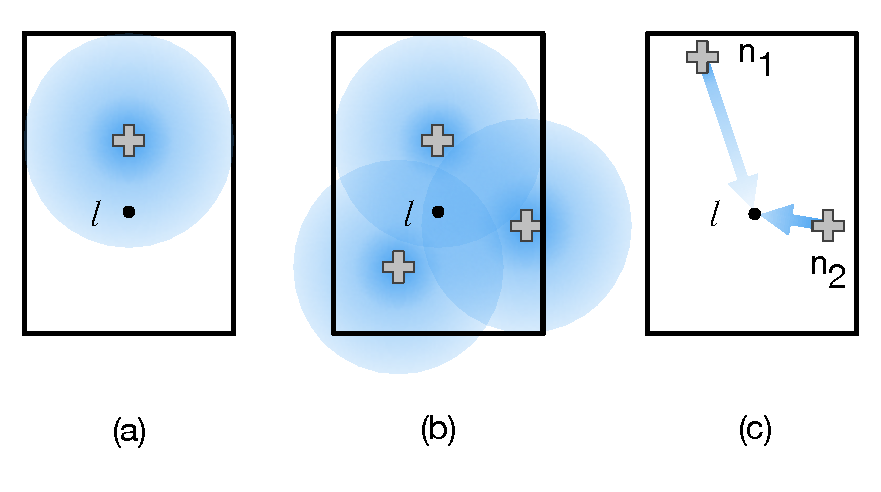
\includegraphics[scale=0.67]{coverage.pdf}
\caption[Example of indoor location covered in single, trilateration and fingerprinting mode.]{Sample floor-plans with a location $l$ covered (a) in single mode, (b) for trilateration, and (c) for fingerprinting where $rss_{l,1} < rss_{l,2}$.}
\label{fig:coverage}
\end{figure}

The comparison is usually performed by a classification algorithm using the Euclidean distance of the vectors, since $rss$ vectors with a small Euclidean distance between them are more likely to be close also in the physical space. We have defined as \(rss_{l,n}\) the signal strength received at location \(l\) from a node $n$. The Euclidean distance between $\vec{rss_a}$ and $\vec{rss_b}$, both composed by \(k\) received signals, and collected respectively in location \(a\) and \(b\) is defined as:

\begin{equation}\label{eq:E}
E(a,b)=\sqrt{(rss_{a,1} - rss_{b,1})^2 + ... + (rss_{a,k} - rss_{b,k})^2}
\end{equation}

Consider the vector $\vec{rss_a}$ as the run-time sample, while the vector $\vec{rss_b}$ retrieved from the stored fingerprint. The smaller is the \(E(a,b)\), more confident is the localization system approximating current location of \(a\) with the stored location of \(b\).

\begin{figure}
\centering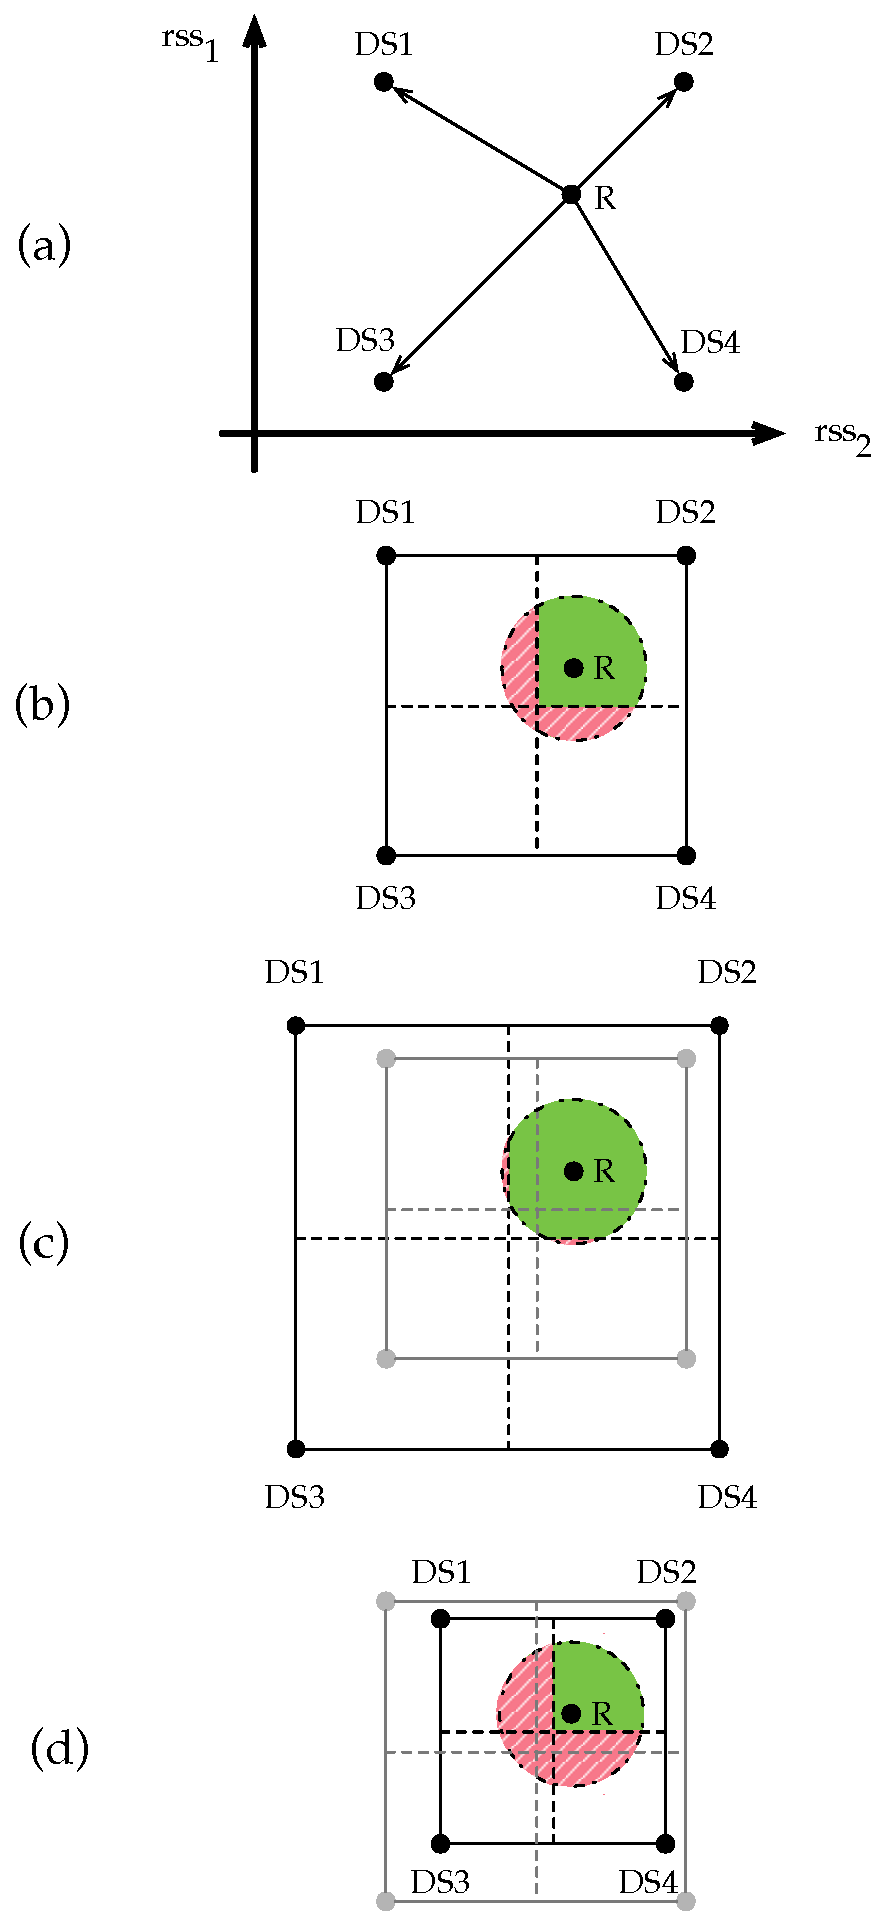
\includegraphics[scale=0.51]{example.pdf}
\caption[Relation between localization accuracy and RSS samples Euclidean distance.]{In diagram (a) bi-dimensional elements of the localization dataset are represented in Cartesian coordinates corresponding to components $rss_1, rss_2$. A run-time sample $R$ is showed in (b) where its circular area delineates signal fluctuations. Green area is proportional to the probability of correct localization, while red dashed area represent wrong localizations. In diagram (c) the Euclidean distance has been increased, thus improving the correct localization; diagram (d) shows the opposite effect.}
\label{fig:fing_example}
\end{figure}

It has been demonstrated that maximizing the Euclidean distances of the $rss$ arrays between all sampling points, the positioning accuracy of wireless localization systems can be improved \cite{Zhao2008, He2011}.
In Figure~\ref{fig:fing_example} is reported a graphical demonstration of the aforementioned statement. Take as an example a dataset ($DS1, DS2, DS3, DS4$) of stored $\vec{rss}$ vectors, where each vector is bi-dimensional ($K=2$) and coupled with the corresponding physical position. Fig.~\ref{fig:fing_example}.a shows each element of the database where the Cartesian coordinates corresponds to components $rss_1, rss_2$. Although the plane does not represent the physical area of the floor-plan, database elements that are near between them are more likely to be close also in the physical space. Given a run-time element $R$, each arrow represents the Euclidean distance $E(R,DS_i)$ from the surrounding dataset elements. A localization algorithm can exploit the Nearest Neighbor technique to approximate the position of $R$ with the nearest dataset element. Unfortunately, the run-time $rss$ measurement of $R$ will not be constant over time, but will experience continuous fluctuations due to environmental noise. These fluctuations make the sample $R$ move randomly to the surrounding points. Suppose that $DS2$ is the nearest points to $R$ in the physical space. Fig.~\ref{fig:fing_example}.b shows with a green area the probability to assign $R$ the correct (or more accurate) position, while a red (with line pattern) area represents the probability to get a wrong position from the system. Fig.~\ref{fig:fing_example}.c demonstrates how an increase in the $rss$ Euclidean distance between sampling points increase the red area and the accuracy of the localization, while in Fig.~\ref{fig:fing_example}.d an Euclidean distance reduction will lead to poorer localizations.\\



The received signal strength has been estimated using the The WINNER II path loss model \cite{Kyosti2008}:

\begin{equation}\label{eq:rss}
PL = A ~ \log_{10} (d[m]) + B + C \log_{10} (\frac{f_c [GHz]}{5.0}) + X
\end{equation}

%--------Nel caso differenziare LOS e NLOS con disegno---------

where \(PL\) is the signal path loss (in dB), \(f_c\) is the frequency in GHz, \(d\) is the distance between the transmitter and the receiver location in meters. Values of coefficients $A$, $B$, $C$, $X$ change depending on LOS (Line-Of-Sight) or NLOS (Non-Line-Of-Sight) propagations, and are reported in table \ref{tab:pathloss}. The propagation model has been used in fingerprinting coverage to maximize the Euclidean distance of the $rss$ vectors between a location and its surrounding points, with the aim of improve the localization accuracy of the system.

\begin{table}[h!tb]
\centering
\caption[Values of coefficients depending on LOS (Line-Of-Sight) or NLOS (Non-Line-Of-Sight) propagations.]{Values of coefficients depending on LOS (Line-Of-Sight) or NLOS (Non-Line-Of-Sight) propagations. Values have been taken from the WINNER II path loss model \cite{Kyosti2008}.}
\label{tab:pathloss}
\def\arraystretch{1.3}
\begin{tabular}{ | l | l |}
    \hline
    \multicolumn{1}{|c|}{\bfseries Scenario} & \multicolumn{1}{c|}{\bfseries Path Loss Coefficients} \\ \hline
    $LOS$ & $A=18.7, B=46.8, C=20$ \\ \hline
    $NLOS$ & \pbox{5cm}{
              $A=36.8, B=43.8, C=20$ \\
              $X=5(n_w-1)$ (light walls)\\
              $X=12(n_w-1)$ (heavy walls)
              } \\
    \hline
    \end{tabular}
    \end{table}

The two-dimensional space of the floor plan is discretized with a length unit (default is 1\(m\)) that is chosen by the user during the map specification phase.\\
As we have said, in addition to location coverage, also nodes connectivity has been modeled. In our model, a sensor node $n$ is connected if exist a connected path to the gateway node. To ensure the connectivity of the whole network, the following equation must hold.

\begin{equation}\label{eq:all_conn}
\forall n \in N, connected(n, gateway) = true 
\end{equation}
where
\begin{equation}\label{eq:connected}
\begin{gathered}
connected(n,n') \stackrel{def}{=} |(n,n')| \leq min(h,h')\\
\lor ~ \exists ~ n_1, \dots, n_i \in N ~ (1 < i),\\
|(n,n_1)| \leq min(h,h_1)\\
\land ~ |(n_1,n_2)| \leq min(h_1,h_2) ~\land ~ \dots\\
\lor ~ |(n_i,n')| \leq min(h_i, h')
\end{gathered}
\end{equation}

Connected networks are managed by our allocation algorithm in the same way of non-connected networks, with the following exception:
\begin{itemize}
\item first, a manual gateway nodes allocation is required;
\item during nodes allocation, deployable points $J$ are restricted to locations $j'$ such that \(connected(n_{j'}, gateway) = true\);
\item during deployment optimization, nodes moves are considered feasible only within the connected area.
\end{itemize}

\begin{table}
\centering
\label{tab:notation}
\caption{Notation and meaning of symbols used for the model.}
\begin{tabular}{ | l | l |}
    \hline
    \multicolumn{1}{|c|}{\bfseries Notation} & \multicolumn{1}{c|}{\bfseries Meaning} \\ \hline
    $L$ & set of monitoring locations \\ \hline
    $J$ & set of deployable locations \\ \hline
    $c_t$ & cost of a node of type $t$ \\ \hline
    $r_t$ & sensing range of a node of type $t$ \\ \hline
    $h_t$ & communication range of a node of type $t$ \\ \hline
    $target$ & coverage rate of $L$ required by user (\%) \\ \hline
    $n_{jt}$ & nodes of type $t$ allocated in $j$ \\ \hline
    $rss_{l,n}$ & signal strength received in $l$ from $n$ \\ \hline
    $\vec{rss_a}$ & vector of all the $rss_{a,n}$ values collected in $a$ \\ \hline
    $E(a,b)$ & Euclidean distance between $\vec{rss_a}$ and $\vec{rss_b}$\\ \hline
    $D_l$ & set of locations no more distant than $d$ from $l$ \\ \hline
    $z$ & average signal space Euclidean distance \\ \hline
    $Z$ & objective function\\ \hline
    $b_l$ & reward earned for covering location $l$\\ \hline
    $w_l$ & reward weighted on the node cost\\ \hline
    $x_{jt}$ & allocation of node with type $t$ in $j$ (binary) \\ \hline
    $a_{ljt}$ & reachability of $n_{jt}$ from location $l$ (binary) \\ \hline
    $k$-coverage & number of reference nodes required by the system \\ \hline
    $k_l$ & current number of reference nodes covering $l$\\ \hline
    $S$ & minimum signal space Euclidean distance threshold \\ \hline
    $s_{min}$ & minimum number of node moves in \emph{shaking} procedure\\ \hline
    $s_{max}$ & maximum number of node moves in \emph{shaking} procedure\\ \hline
    $Rmax$ & number of restarts of the \emph{VNS} algorithm\\ \hline


    \end{tabular}
\end{table}

\section{Covering Location Algorithm}\label{subsec:placing}
The covering location algorithm has the purpose of placing an optimal set of nodes on the building floor plan. We have decided to implement a modified version of the Multimode Covering Location Problem \cite{Colombo2016}, a generalization of the MCLP. Using a quite general and flexible reformulation of the covering problem, we have been able to adapt the algorithm at the different covering techniques described previously.

The positioning algorithm is composed by a first \emph{Greedy} procedure, whose solution is then improved by a \emph{Variable Neighborhood Search} (VNS) algorithm.
The positioning algorithm evaluates different solutions using a reward \(b_l\), that is defined for each location $l$ and will be earned only for the locations covered in that particular solution. The value of the reward depends on the coverage technique:

\begin{itemize}
\item Single coverage: the reward \(b_l\) will be earned if there is at least one node that covers $l$.
\item Trilateration: the reward \(b_l\) will be earned if there are at least three nodes that cover $l$.
\item Fingerprinting: since this technique is often considered to be a trade-off (in cost and accuracy) between single coverage and trilateration, we decided that the reward \(b_l\) will be earned if there are at least two nodes that covers $l$.
\end{itemize}

%--------- distanza euclidea dai surrounding locations ----------
As we have said, in order to maximize the localization accuracy of the system it's possible to increase the signal space Euclidean distance between the target points.
Consider the mean Euclidean distance between the received $rss$ vector in a certain location \(l\), and the surrounding locations $s$ within a certain distance \(d\):
\begin{equation}\label{eq:fing}
\begin{gathered}
\frac{1}{\mid D_l \mid} \sum\limits_{s \in D_l} E(l,s)\\
D_l = \{s \in L \mid distance(l,s)  \leq d\}
\end{gathered}
\end{equation}
The distance $d$ is used to restrict the $rss$ comparison and diversification only to the locations that are more likely to be erroneously confuse with $l$ by the localization system. Fig.~\ref{fig:rssdiv} shows an example of how the Euclidean distance of a location is compared to a neighbor location.


\begin{figure}
\centering
\begin{minipage}{0.63\textwidth}

$
\begin{gathered}
\vec{rss_l} = \langle rss_{l,1}, rss_{l,2} \rangle = \langle-84, -72\rangle ~ [dB] \\
\vec{rss_s} = \langle rss_{s,1}, rss_{s,2} \rangle = \langle-67, -41\rangle ~ [dB] \\[5pt]
E(l,s) = \\ = \sqrt{(rss_{l,1} - rss_{s,1})^2 + (rss_{l,2} - rss_{s,2})^2} = \\
= \sqrt{(-84-(-67))^2 + (-72-(-41))^2} = \\ = 35.3 ~ [dB]
\end{gathered}
$

\end{minipage}%%%
\begin{minipage}{0.37\textwidth}
\centering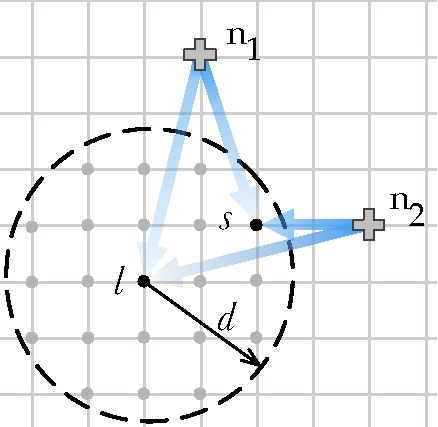
\includegraphics[width=\linewidth]{rssdiv.pdf}
\end{minipage}
\caption{Regular grid showing how is computed the mean Euclidean distance between the received $rss$ vectors in a certain location \(l\), and the surrounding locations $s$ within a certain distance \(d\).}
\label{fig:rssdiv}
\end{figure}

We define the average signal space Euclidean distance $z$:
\begin{equation}\label{eq:z1}
z = \frac{ \sum\limits_{l \in L} \sum\limits_{s \in D_l}\frac{E(l,s)}{|D_l|}}{|L|}
\end{equation}

The term $z$ will be used by the \emph{Greedy} procedure to produce a first solution with a reasonable allocation of nodes. Then, the value of $z$ should be increased as much as possible to provide good localization accuracy to the system. However, maximize only the average does not seems fair enough, since a good system should provide a certain level of accuracy homogeneously among the target area. So we defined the objective function as difference between the term $z$ and the signal space Euclidean variance:

\begin{equation}\label{eq:Z1}
Z = z - \sqrt{\sum\limits_{l\in L}\left(\sum\limits_{s\in D_l}\frac{E(l,s)}{\mid D_l \mid}\right)^2}
\end{equation}

Maximizing the objective function $Z$, the intention is to provide as many target location as possible with a high signal space Euclidean distance with respect to the surrounding locations.


As we have previously introduced, we represent with \(L\)  the entire set of location to be covered, while with \(J\) the set of possible positions where nodes can be placed. By default, \(L = J\) and nodes can be positioned everywhere; however its possible to restrict the \(J\) set only to specific candidate points, that represent for example power outlets or Ethernet sockets.
The problem of find a near-optimal set \(N\) of nodes \(n_{jt}\) (each one located in $j$ and having a type $t$) with a coverage rate $f(N)$ that satisfies the $target$ coverage, can be formalized as follows.
\begin{equation}\label{eq:Z}
\max Z = z - \sqrt{\sum\limits_{l\in L}\left(\sum\limits_{s\in D_l}\frac{E(l,s)}{\mid D_l \mid}\right)^2}
\end{equation}
\begin{equation}\label{eq:cov}
f(N) \geq target
\end{equation}
\begin{equation}\label{eq:one}
\sum\limits_{t \in T} x_{jt} \leq 1 \quad \forall j \in J
\end{equation}
\begin{equation}\label{eq:x}
x_{jt} = 1 \quad \iff n_{jt} \in N
\end{equation}
\begin{equation}\label{eq:f}
f(N)= \lvert L \rvert / \sum\limits_{l \in L} y_l
\end{equation}
\begin{equation}\label{eq:y}
\begin{cases}
y_l \leq \sum\limits_{j \in J}\sum\limits_{t \in T} a_{ljt} x_{jt} \quad \forall l \in L ~ (single)\\
2~y_l \leq \sum\limits_{j \in J}\sum\limits_{t \in T} a_{ljt} x_{jt} \quad \forall l \in L ~ (fingerprinting)\\
3~y_l \leq \sum\limits_{j \in J}\sum\limits_{t \in T} a_{ljt} x_{jt} \quad \forall l \in L \quad (trilateration)\\
\end{cases}
\end{equation}

The decision variable $x_{jt}=1$ represents the allocation of a node of type $t$ in location $j$; $a_{ljt}$ is equal to $1$ if location $l$ can be reached by a node of type $t$ placed in $j$, and $a_{ljt}=0$ otherwise. $y_l=1$ if location $l$ is covered, $y_l=0$ otherwise. The constraint \eqref{eq:one} fixes to one the maximum number of nodes that can be located in each site.

\subsection{Greedy Procedure}\label{subsec:greedy}
The positioning algorithm starts with a \emph{Greedy} procedure with the purpose of find a reasonable number of reference nodes, for both coverage and localization accuracy. The procedure generate a first solution \(N\) positioning a set of \(k\) = $\lvert N \rvert$ nodes, each one with a type \(t \in T\).
For all three coverage techniques, the reward $b_l$ is weighted with the cost of the current node $n^*$ selected for the coverage:
\begin{equation}\label{eq:w}
w_l = \frac{b_l}{ c_t}; \quad \{n^*=n_{jt} ~ \land ~ distance(j,l)  \leq r_t\}
\end{equation}
The weighted reward $w_l$ will be used by the \emph{Greedy} algorithm so that on equal covered area, the cheapest node type has the priority over the others.
We denote as \(L_{jt}\) the subset of locations that are reachable by a reference node \(n\) of type \(t\) placed at location \(j\). At each iteration, the algorithm places a node \(n\) of type \(t^*\) at position \(j^*\) that covers the subset of locations \(L_{j^*t^*}\) with the maximum reward. The term
\begin{equation}\label{eq:kcov}
1 - \frac{k_l}{k-coverage}
\end{equation}
is used to prioritize the covering of locations with a lower 'temporary' \mbox{$k$-coverage} (called $k_l$) with respect to the \mbox{$k$-coverage} required by the current techniques. In this way, \emph{Greedy} procedure tends to avoid the placement of nodes very close to one other which can lead, especially for trilateration systems, to poor localization accuracy.
It's important to notice that the purpose of the \emph{Greedy} procedure is to find a reasonable number of nodes for the localization service. The starting positioning is made on a best-effort basis, that will be improved by the successive \emph{VNS}.
After a node allocation, all subsets \(L_{jt}\) are updated according to the coverage technique. In trilateration for example, a location \(l\) is removed from \(L_{jt}\) only if there exist, other than the current  \(n_{j^*t^*}\), other two nodes that are already covering \(l\).

\begin{algorithm}
\caption{\(Greedy(L, J, T, w, target)\)}
\begin{algorithmic}%[1] row numbers
%\Procedure{MyProcedure}{}
\label{alg:greedy}
\State $N := \varnothing$;
\State $L_{jt} := \{l \in L \mid l$ is covered by node in \(j\) with type \(t\)\};
\While{$(f(N) < target) \land (z < S)$}
\State $j^{*} := \argmax{j \in J} \sum\limits_{l \in L_{jt}}w_l ~ (1 - \frac{k_l}{k-coverage})$;
\State $t^{*} := \argmax{t \in T} \sum\limits_{l \in L_{jt}}w_l ~ (1 - \frac{k_l}{k-coverage})$;
\State $N := N \cup \{n_{j^*t^*}\}$;
\State $L_{jt} := L_{jt} \setminus L_{j^*t}$ for all $j \in J$;
%\State update $coverage$;
\EndWhile
\State \Return $N$;
%\EndProcedure
\end{algorithmic}
\end{algorithm}

The \emph{Greedy} procedure ends when the $target$ coverage is satisfied, and when the average signal space Euclidean distance $z$ reaches the threshold $S$. In our implementation we set the threshold $S=4.5$ that has been proven to be the average Euclidean distance for which the positioning error is limited to 2 meters \cite{He2011}.
How we will see in the {\hyperref[cap:results]{experimental results chapter}}, the \emph{Greedy} procedure is able to provide an average Euclidean distance not so far from the final best known. However, thanks to the low complexity of the \emph{Greedy} procedure, additional time can be used to improve the solution. In addition, the Euclidean distance variance will be strongly improved.

\subsection{Variable Neighborhood Search}
The method called \emph{Variable Neighborhood Search} (VNS) has been used to improve the solution coming from the \emph{Greedy} procedure. The VNS approach empowers the classical local search framework with a restart mechanism that extends the search after a local optimum has been achieved by generating new starting solutions in progressively enlarged neighborhoods of the current best known solution. The key elements of the VNS (reported in algorithm 2) are a starting solution $N$ with a hierarchy of size-increasing neighborhoods, and a local search procedure, i.e., the criterion to select the incumbent solution from the neighborhood. These components are used to restart the search every time that the procedure reaches a local optimum.
Figure~\ref{fig:algorithm} shows an overview of the VNS process. 
\begin{figure}[h!tb]
\centering\includegraphics[scale=0.25]{algorithm.pdf}
\caption{Location Algorithm. The solution found by the \emph{Greedy} algorithm is improved applying iteratively a \emph{Local Search} for an optimal solution and a \emph{Shaking} procedure that perturbs the current solution.}
\label{fig:algorithm}
\end{figure}
A first local search procedure is applied to the solution produced by the \emph{Greedy} procedure. At each iteration, the \emph{shaking} procedure is used to generate a new starting solution, which is then improved by the execution of the local search. The shaking procedure perturbs \(s\) node allocations of the current solution \(N^*\) replacing them with \(s\) unused nodes. The behavior of the shaking parameter \(s\), that depends on the result of the local search, is explained in Figure~\ref{fig:shaking}. 
\begin{figure}[h!tb]
\centering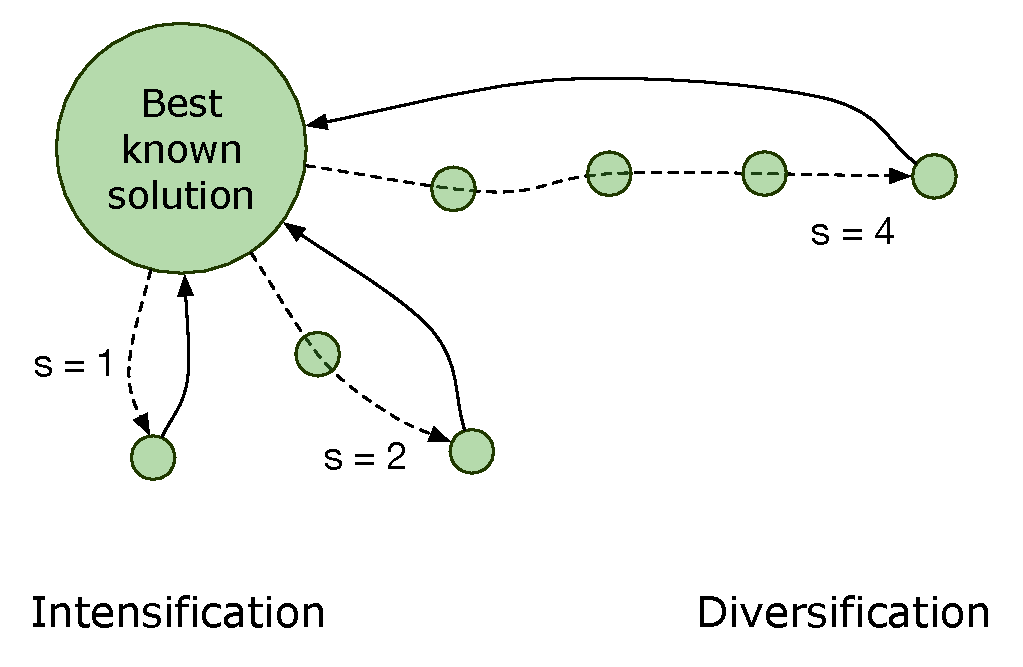
\includegraphics[scale=0.55]{VNSgraph.pdf}
\caption{Shaking procedure: the parameter $s$ is increased when the solution does not improve (dashed line) and restarts when a new optimum is found (continuous line).}
\label{fig:shaking}
\end{figure}
The parameter \(s\) starts from a minimum value \(s_{min}\) (in the example \(s_{min} = 1 \)) and every time that the local search does not improve the best known solution, \(s\) is increased by 1. Differently, when the local search succeeds, the best solution \(N^*\) is updated and \(s\) goes back to \(s_{min}\).

The purpose of the shaking procedure is to first explore new starting solutions that are more similar to the best known result, so that the search is \emph{intensified} in a promising neighborhood of the entire domain. If these local searches fail, the shaking procedure moves the search from intensification to \emph{diversification}, generating starting solutions that are more and more different from the incumbent one. Whenever a new best solution is found, the shaking procedure comes back to \(s_{min}\), to intensify the search near the just updated \(N^*\). In principle, the shaking parameter \(s\) can be increased until $k=\lvert N^* \rvert$, changing all the node allocations. However, we experimented running different configurations that excessively moving away from the best known solution can be unproductive, causing a useless waste of computational time. We have fixed a reasonable value of \(s_{max} = \floor{\frac{2}{3}k}\).

\begin{algorithm}
\caption{\(VNS (L, J, T, w, target, s_{min}, s_{max}, R_{max})\)}
\begin{algorithmic}%[1] row numbers
\label{alg:vns}
%\Procedure{MyProcedure}{}
\State $N:=Greedy(L, J, T, w, target)$;
\State $N^{0}:=LocalSearch(L, J, T, w, target)$;
\State $N^* := N^0$;
\State $s := s_{min}$;
\For{$r:=1$ to $R_{max}$}
\State $N:= Shaking(N^*, s, L, J, T, w, target)$
\State $N^0:= LocalSearch(L, J, T, w, target)$
\If{($Z(N^0) > Z(N^*)$)}
\State $s:=s_{min}$;
\State $N^*:=N^0$;
\Else
\State $s:=s+1$;
\If{($s > s_{max}$)}
\State $s:=s_{min}$;
\EndIf
\EndIf
\EndFor
\State \Return $N^*$;
%\EndProcedure
\end{algorithmic}
\end{algorithm}

The VNS algorithm terminates when the total number of restarts reaches a given value $R_{max}$.
%In our implementation, we have decided to make the value of $R_{max}$ vary adaptively, depending on the size of the problem instance ($\lvert J \rvert$, $\lvert T \rvert$). 

As we have said, the local search is the heuristic that proceeds from an initial solution to its neighborhood by a sequence of local changes, trying to improve each time the value of the objective function until a local optimum is found.
The neighborhood of the adopted approach is given by cyclic sequences of moves, where each move consists in locating a new node, removing a node or changing the type of the node. A cyclic move is considered feasible only if the new covering rate respects the \emph{target} coverage, and the total cost of the solution does not increase. Of course, each site must continue to hosts at maximum one node (constraint equation \eqref{eq:one}). A cyclic move can be visualized on a graph $G=(N,A)$, where each node of the graph is a possible allocation of a hardware node. Each node of the graph is characterized by a location $j$, and a state that indicates if the node is active or inactive. A node $n_{jt}$ currently allocated in location $j$, is represented on the graph with an active node $n_j$, labeled with its hardware type $t$. Note that index $t$ does not appear because at most one type can be active in each node, and the type is specified by the label. Inactive nodes are instead left unlabeled. An arc ($n_j, n_k$) can represent:
\begin{enumerate*}[label={(\arabic*)}]
\item the allocation of a hardware node in site $j$, if $n_j$ is inactive and $n_k$ is active;
\item the removal of a hardware node in site $j$, if $n_j$ is active and $n_k$ is inactive;
\item an hardware node $n_j$ changing its hardware type, if both nodes are active.
\end{enumerate*}
In both (1) and (2), the new node takes the hardware type of the head label ($t$ of $n_k$). A cyclic exchange corresponds to a directed cycle on the improvement graph, as depicted in Figure~\ref{fig:graph}. 
\begin{figure}[h!tb]
\centering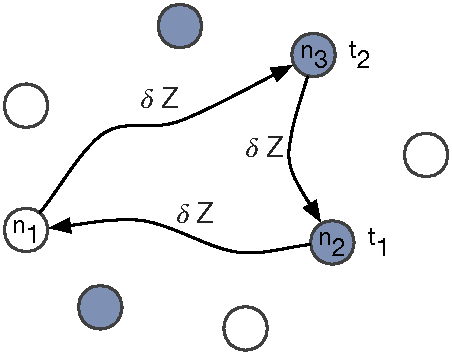
\includegraphics[scale=0.7]{graph.pdf}
\caption{Improvement Graph: colored nodes represent current allocations, while empty nodes are possible allocations. All active nodes are labeled with their corresponding type. Each arc is a change (move) on the allocations.}
\label{fig:graph}
\end{figure}
Each move, and so each arc ($n_j, n_k$), determines a variation $\delta Z$ in the value of the objective function $Z$. The purpose is to represent a group of moves so that a cyclic exchange represents an increase in the current objective function. However the total variation $\delta Z$ is non additive with respect to the sequence of $\delta Z$ values coming from single moves. This is caused by the interdependence between different hardware nodes with overlapping covering regions, that lead to non-additive moves. To overcome this drawback, every cycle has been evaluated using an own temporary function $Z'$ updated step by step from the end of the path to its starting node. In this way, all the cycles with a positive total weight bring improvements on the starting solution.

The search for the cyclic exchange with maximum weight is performed with exhaustive breadth-first exploration of the paths of graph $G$.


%\section{Experimental Results}\label{sec:results}

% \section{Limitations, future works and Conclusions}
% A first limitation of the proposed approach reside in the propagation model used to compute near-optimal solutions for localization systems. The model implemented is site-specific, and take in consideration walls for LOS and NLOS propagations. However the approach do not consider refraction or diffraction effects. Another limitation is the inability of the system to model the signal propagation between different floors of the building, managing each level independently.\\
% For future work, we plan to improve the system with an indoor signal propagation model able to consider refraction and diffraction effects of the indoor environment like walls and floors. In addition, we'll try to apply the model to 3D designing tools, becoming suitable also for multi-floor environments.
%This model keep into account a floor penetration loss factor, becoming applicable also for multi-floor environments.


\section{Conclusions and Future Work}
In this chapter, we tried to explain the challenges faced by designers during the installation of smart building systems that require the positioning of several hardware nodes. A common limitation of existing models is the lack of a convenient way to specify geometric information of the indoor map. This also leads to the employment of less accurate general models for signal propagation, instead of site-specific models. The design phase is made	 more difficult by the availability on the market of different hardware nodes, with different power transmissions and costs.

For these reasons we propose an integrated tool for both floor plan specification and node positioning, developed within an \mbox{open-source} CAD environment extensible through plug-ins. The tool is able to provide a near-optimal solution of node allocations, possibly with mixed types, with the aim to reduce the installation costs. The results suggest that, for most of the problem instances, a solution can be obtained in a reasonable execution time. Depending on the available hardware types, total cost of the solution could be improved moving from homogeneous to mixed type allocation.

A limitation of the proposed approach resides in the propagation model used to compute near-optimal solutions for localization systems. The model implemented is site-specific, and take in consideration walls for LOS and NLOS propagations. However the approach do not consider refraction or diffraction effects. Another limitation is the inability of the system to model the signal propagation between different floors of the building, managing each level independently.
For future work, we plan to improve the system with an indoor signal propagation model able to consider refraction and diffraction effects of the indoor environment like walls and floors. In addition, we'll try to apply the model to 3D designing tools, becoming suitable also for multi-floor environments.
%
% ------------------------------------------------------------------------ %
% !TEX encoding = UTF-8 Unicode
% !TEX TS-program = pdflatex
% !TEX root = ../Tesi.tex
% !TEX spellcheck = it-IT
% ------------------------------------------------------------------------ %
%
% ------------------------------------------------------------------------ %
% 	NOME CAPITOLO
% ------------------------------------------------------------------------ %
%
\chapter{Experimental Results}
%
\label{cap:results}

In this chapter are reported the experimental analysis performed to validate the work done for this thesis.\\
First, section \ref{sec:bs-test} contains the experiments conducted over the occupancy monitoring system (BlueSentinel) proposed in chapter \ref{cap:bluesentinel}. The system has been evaluated in terms of accuracy of the localization, responsiveness of the detection and power consumption of the mobile application developed. As we will see, the results confirmed that the proposed approach is suitable to obtain the occupancy monitoring information with a good quality.

Later, section \ref{sec:CAD-test} contains the results obtained from the automatic deployment tool reported in chapter \ref{cap:cad}. The tool has been used to deploy a localization system different from BlueSentinel (a beacons based system) in order to test the general-purpose functionalities and the ability to model different systems. The results include the computational experience of the tool, such as the execution times, and some evaluation metrics of the resulting deployed configuration. These include the cost-effectiveness and the accuracy of the resulting localization system with respect to configuration obtained with different approaches from literature.

\section{Occupancy Monitoring Evaluation}
\label{sec:bs-test}
The occupancy monitoring system presented in chapter \ref{cap:bluesentinel} has been evaluated using data collected from a real-world environment. The system has been set up inside the NECST Lab, located at the basement of DEIB department at Politecnico di Milano.\\
The dimension of the test-bed is 198 squared meters ($9x22m$). The area is subdivided by walls in three separate spaces: a relax room for coffee breaks, a room for meetings and talks, and an open-space with desktop stations.\\
For the installation of the system, before proceed with the training procedure, the administrator needs to identify the regions in which the floor-plan will be partitioned. The dimension of each region will determine the spatial resolution of the occupancy monitoring, as stated in section \ref{sec:occupancy-metrics}. In our setup, we decide to identify a single region for each room in the case of coffee and meeting rooms, while halving the open-space for two main reasons. First, the open-space is large roughly two times the dimension of the other rooms, and this way each region has similar dimensions. Second, because the open-space presents a functional division in two parts between stations occupied by computer security students and by computer architectures students.

The resulting configuration has been used to detect the presence of a user, classifying its position in the best fitting region based on the collected data. The performance and the accuracy have been evaluated comparing the classification results with the observed ground truth location of the test user.

\begin{figure}[h!tb]
\centering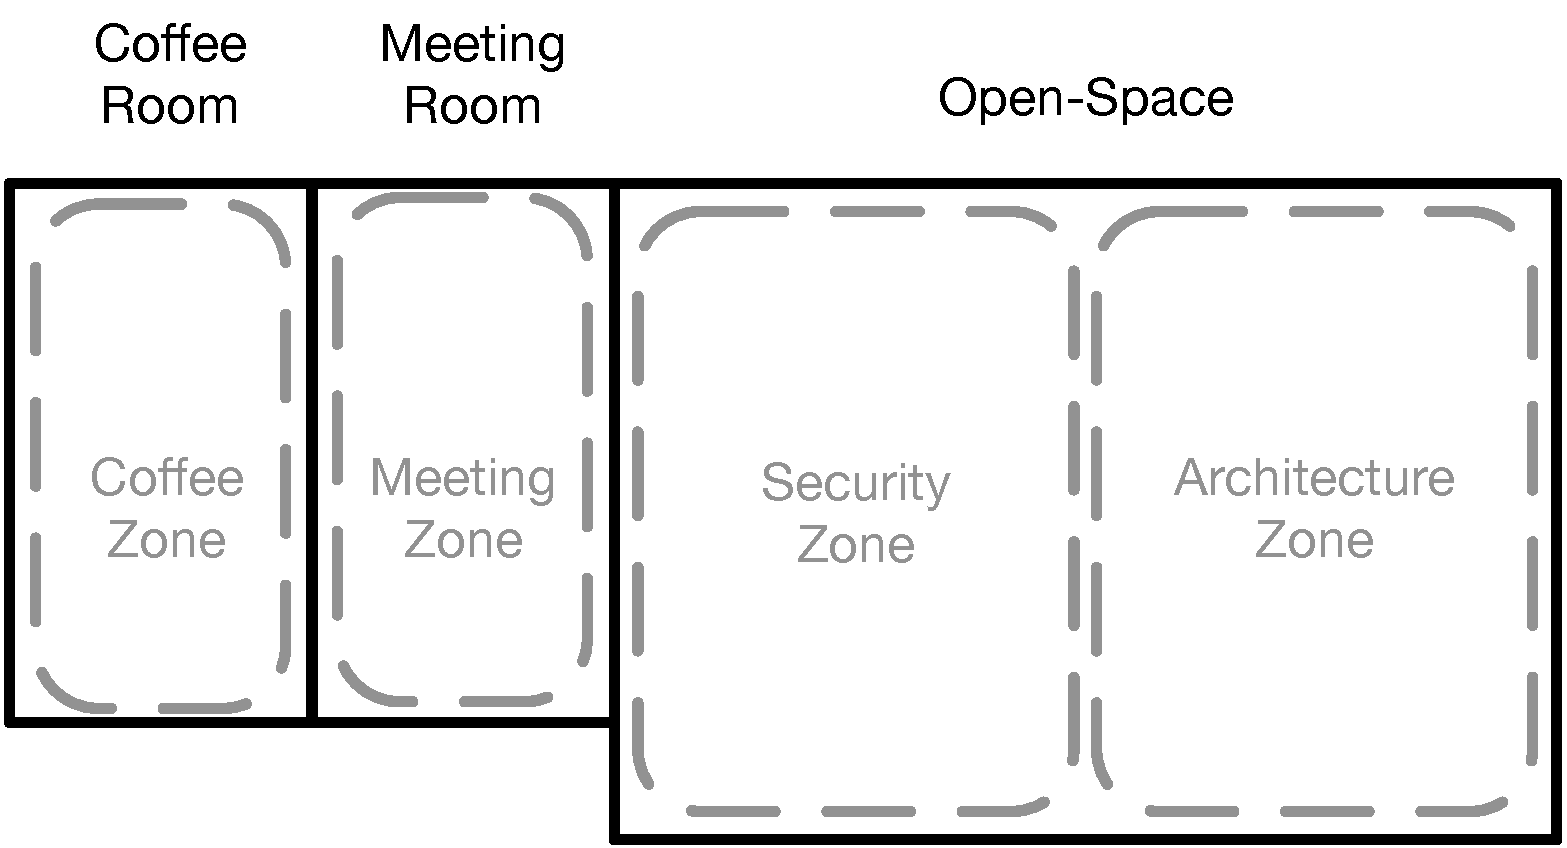
\includegraphics[width=\linewidth]{necst-regions.pdf}
\caption[Floor-plan rooms of the experimental testbed and the regions identified for the occupancy detection.]{Floor-plan rooms of the experimental testbed and the regions identified for the occupancy detection.}
\label{fig:regions}
\end{figure}

\subsubsection{Indoor Environment}
\label{test-env}
The space used for all the test reported in this chapter is that introduced previously and showed in figure \ref{fig:regions}. The perimeter of the laboratory is constituted by reinforced concrete walls, while the walls dividing the three rooms are made in plasterboard.

From the point of view of signal propagation, the environment is characterized by a high level of noise. The space is in most cases high populated, reaching 30 people at the same time ($\approx 1 ~ person / 5m^2$).
Many of these occupants bring in laboratory devices such as smartphones, smartwatches and Bluetooth headphones.
The laboratory equipment includes a high number of wireless devices, such has WiFi access points, Bluetooth beacons, and wireless development boards. Other devices that could interfere with signal transmission and analysis are two microwaves, a projector and a 3D printer.

Summarizing, the wireless communication in our testbed is characterized by lossy and noisy channels, representing a worst case for accuracy measurements.

\subsubsection{Smartphones}
\label{sec:test-phones}
To test the accuracy of the occupancy monitoring system, two Android devices have been employed.
\begin{itemize}
\item The first is a Google Nexus 5 running Android 6.0.1. This device has been used to perform the system training, and to test the localization accuracy when the runtime device is the same of the training.
\item The second is a Samsung I9300 (Galaxy S3) running Android 4.3. This device has been used to test the localization accuracy when the runtime device is different from the device employed for the training.
\end{itemize}
The mobile application running on the devices during test has been explained in detail in section \ref{sec:app}.
The Samsung device has also been used, through a customized battery, to measure precise power consumptions of the mobile application.

%TODO: accennare il fatto che rasp non ha antenna esterna
\subsubsection{WSN prototype}
\label{sec:test-wsn}
Each node of the wireless sensor network has been implemented with Raspberry Pi boards version 3. The operating system running on each board is the Raspbian 4.4 (September 2016) based on Debian 7.0. The software routine running on each sensor node has been detailed in section \ref{sec:wsn}.\\
%posizionamento e quantità dei nodi con immagine (o sketch o cad)
The position and the amount of nodes employed has been obtained using our automatic CAD tool detailed in chapter \ref{cap:cad}. The sketch in figure \ref{fig:wsn-sketch} shows the resulting nodes allocation of four nodes.

\begin{figure}[h!tb]
\centering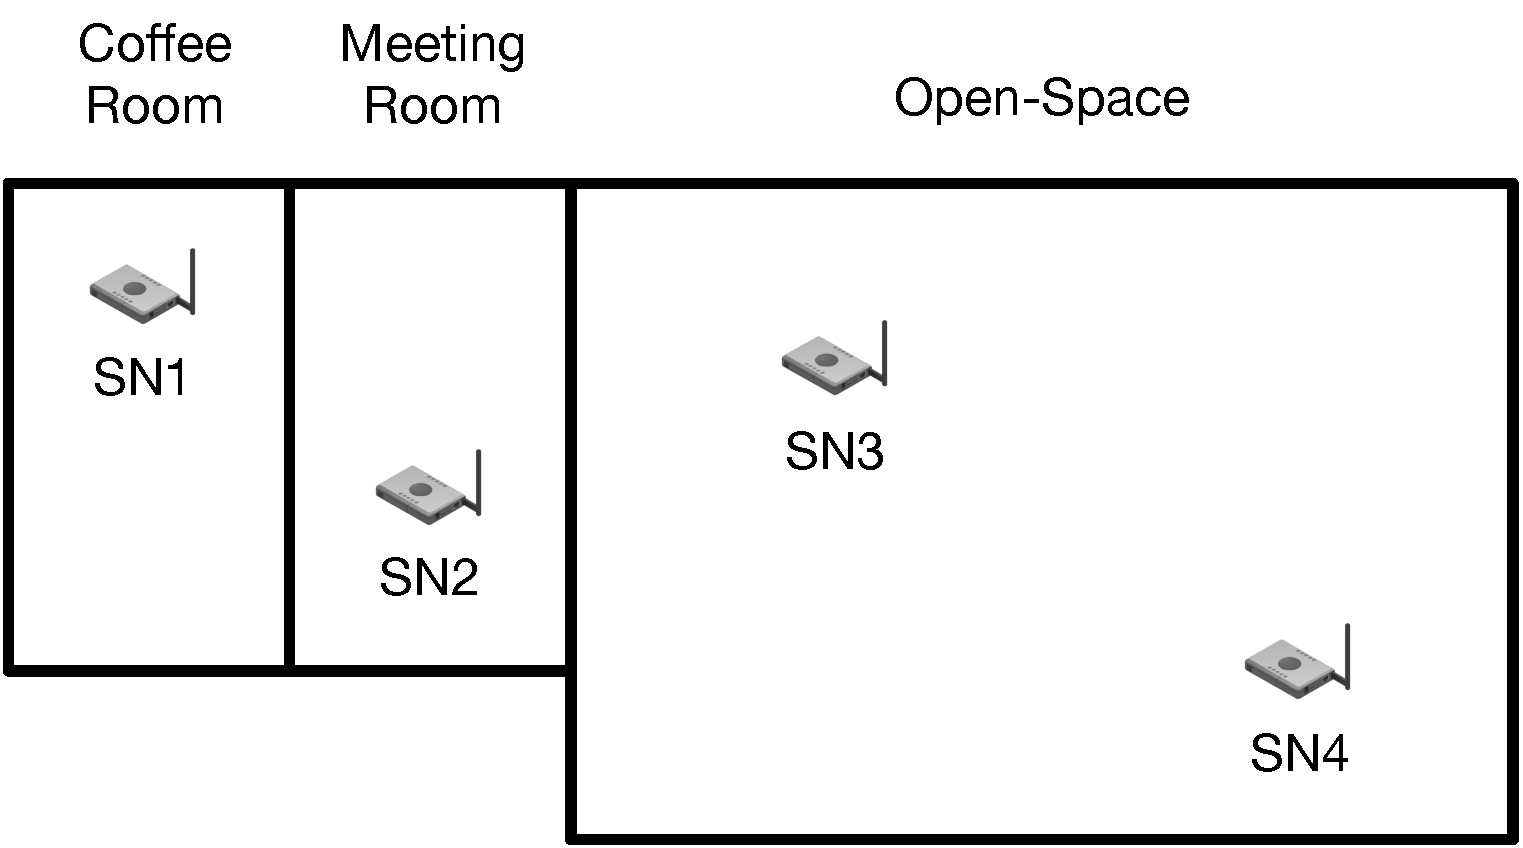
\includegraphics[width=\linewidth]{necst-wsn.pdf}
\caption[Sensor nodes allocation on the floor-plan of the experimental testbed for the occupancy detection.]{Sensor nodes allocation on the floor-plan of the experimental testbed for the occupancy detection.}
\label{fig:wsn-sketch}
\end{figure}

Some of the nodes have been connected to the building LAN using Ethernet sockets, while other were connected using WiFi.
%Power consumption of sensor nodes has been measured using the energy logger 4000 by Voltcraft.
% TODO: togliere o finire

\subsubsection{Back-end}
\label{sub:test-backend}
Since the localization algorithm is performed on the back-end side, the amount of computational resources and the response time of the cloud service affect the responsiveness of the occupancy detection.\\
In our case, the system back-end relies on a cloud platform
\footnote{Parse Cloud service: \url{https://parse.com/}}
that provides free services until a certain load (e.g. the number requests and pushes), while applying different pricing for superior plans.
For this reason, delays of our system at the back-end layer are mainly caused by the plan limits of the cloud service; moving to a custom deployed server with higher computational resources can improve the overall responsiveness.

\subsection{Localization Accuracy}
\label{sec:loc-accuracy}
All the results on the classification algorithms presented in this section have been computed by using the data mining tool Weka \cite{Hall2009}.
During the test we move through the four different regions many times in order to collect a big number of statistical samples.
We have conducted a large number of experiments in order to check if people inside (or outside) a region are correctly recognized by the BlueSentinel system and if the proposed approach can be effectively used to determine the number and the identities of the people inside a particular room.
In the next two sections are reported the test results of two classification methods, verifying their ability to classify the occupant in the correct region.

\subsubsection{K Nearest Neighbor}
This section reports the results we have obtained by employing the K-Nearest Neighbors algorithm with K equal to 5.
We have computed this values by using a stratified ten-fold cross validation, because of the high number of samples collected.

\begin{table}
\center
\caption[K Nearest Neighbor classification results obtained using the baseline dataset.]{K Nearest Neighbor classification results obtained using the baseline dataset (sec. \ref{subsec:algorithms}). Same device refers to measurement obtained using the same device for training and testing. Different device refers to measurement obtained using different devices for training and testing.}
\label{tab:knn-baseline}
\begin{tabular}{ |l|l|l| }
  \hline
  \multicolumn{3}{|c|}{\textbf{KNN Classification - Baseline Dataset}} \\
  \hline
  \textbf{Parameter} & \textbf{Same device} & \textbf{different device}\\
  \hline
  Correctly Classified Instances & 749 (86.09\%) & 635 (72.99\%) \\
  Incorrectly Classified Instances & 121 (13.91\%) & 235 (27.01\%) \\
  Total Number Of Instances & 870 & 870 \\
  Kappa statistic & 0.696 & 0.374 \\
  Mean absolute error & 0.139 & 0.270 \\
  Root mean squared error & 0.373 & 0.519 \\
  True Positive Rate & 86.09\% & 72.99\% \\
  False Positive Rate & 13.91\% & 27.01\% \\
  Precision & 86.09\% & 72.99\% \\
  Recall & 86.09\% & 72.99\% \\
  F-Measure & 86.09\% & 72.99\% \\
  \hline
\end{tabular}
\end{table}

The results in table \ref{tab:knn-baseline} refers to classification performed using baseline RSS data (sec. \ref{subsec:algorithms}). The results show that KNN is able to classify the occupant in the correct region with an accuracy of 86\% when its device is the same (or has similar transmission power) with the one employed during training. The classifier seems to perform well even if it is pretty simple, leading to a good precision, recall, F-measure and ROC area. The first two metrics evaluate the impact of false positives and false negatives, while the F-measure takes in account both precision and recall. The higher is this metric, the better is the quality of the classifier. Similarly, the receiver operating characteristic (ROC) characterizes the trade-off between hit rate and false-alarm rate in this noisy environment.\\
However, moving to the runtime dataset collected with a different mobile device (last column in \ref{tab:knn-baseline}), the performance suffers a sensible deterioration. In particular, the accuracy is lower than 73\%. This sensible difference is most likely to be caused by the employment of absolute values of RSS, when instead different devices transmit signals at different power levels.

\medskip
With the aim to solve this issue, another dataset has been evaluated. In this case, elements of the RSS vectors are not considered as absolute values; instead, a differential value between each couple of RSS is computed and used to build the differential vector, as explained in section \ref{subsec:algorithms}.\\
\begin{table}
\center
\caption[K Nearest Neighbor classification results obtained using the differential dataset.]{K Nearest Neighbor classification results obtained using the differential dataset (sec. \ref{subsec:algorithms}). Same device refers to measurement obtained using the same device for training and testing. Different device refers to measurement obtained using different devices for training and testing.}
\label{tab:knn-diff}
\begin{tabular}{ |l|l|l| }
  \hline
  \multicolumn{3}{|c|}{\textbf{KNN Classification - Differential Dataset}} \\
  \hline
  \textbf{Parameter} & \textbf{Same device} & \textbf{different device}\\
  \hline
  Correctly Classified Instances & 757 (87.01\%) & 720 (82.76\%) \\
  Incorrectly Classified Instances & 121 (12.99\%) & 150 (17.24\%) \\
  Total Number Of Instances & 870 & 870 \\
  Kappa statistic & 0.701 & 0.583 \\
  Mean absolute error & 0.118 & 0.159 \\
  Root mean squared error & 0.344 & 0.399 \\
  True Positive Rate & 87.01\% & 82.76\% \\
  False Positive Rate & 13.91\% & 17.24\% \\
  Precision & 87.01\% & 82.76\% \\
  Recall & 87.01\% & 82.76\% \\
  F-Measure & 87.01\% & 82.76\% \\
  \hline
\end{tabular}
\end{table}
The results that refers to classification performed using differential RSS data are reported in table \ref{tab:knn-diff}.
The results show that KNN is able to classify the occupant in the correct region with an accuracy of 87\% when its device is the same (or has similar transmission power) with the one employed during training.
The classifier seems to perform well even if it is pretty simple, leading to a good precision, recall, F-measure and ROC area.\\
As expected, moving to the runtime dataset collected with a different mobile device, the performance are lower ($\approx$ 83\%). However, comparing this result to the previous case of baseline data, the classification accuracy has been increased of almost ten percentage points. The differential data approach reveals to be effective to reduce the hardware dependency of samples, and to reduce the correlation between collected data and runtime device.


\subsubsection{Decision Trees}
\label{test-trees}
In this section are presented the results obtained by using decision trees classification, evaluated with a stratified ten-fold cross validation. The specific algorithm employed is detailed in section \ref{subsubsec:trees}. As shown in table \ref{tab:tree-baseline}, for the baseline dataset, the accuracy of the tree algorithm is very similar to the one obtained with the KNN algorithm (table \ref{tab:knn-baseline}). In particular, the accuracy is slightly lower for same device case (83\%), and almost the same for different device (73.8\%).


\begin{table}
\center
\caption[Decision Trees classification results obtained using the baseline dataset.]{Decision Trees classification results obtained using the baseline dataset (sec. \ref{subsec:algorithms}). Same device refers to measurement obtained using the same device for training and testing. Different device refers to measurement obtained using different devices for training and testing.}
\label{tab:tree-baseline}
\begin{tabular}{ |l|l|l| }
  \hline
  \multicolumn{3}{|c|}{\textbf{Decision Trees Classification - Baseline Dataset}} \\
  \hline
  \textbf{Parameter} & \textbf{Same device} & \textbf{different device}\\
  \hline
  Correctly Classified Instances & 726 (83.45\%) & 642 (73.79\%) \\
  Incorrectly Classified Instances & 144 (16.55\%) & 228 (26.21\%) \\
  Total Number Of Instances & 870 & 870 \\
  Kappa statistic & 0.611 & 0.492 \\
  Mean absolute error & 0.136 & 0.241 \\
  Root mean squared error & 0.369 & 0.491 \\
  True Positive Rate & 83.45\% & 73.79\% \\
  False Positive Rate & 16.55\% & 26.21\% \\
  Precision & 83.45\% & 73.79\% \\
  Recall & 83.45\% & 73.79\% \\
  F-Measure & 83.45\% & 73.79\% \\
  \hline
\end{tabular}
\end{table}

Also for tree based classification, the algorithm has been tested with differential data.
The results show that decisional trees are able to classify the occupant in the correct region with an accuracy of 85\% when its device is the same (or has similar transmission power) with the one employed during training.
The classifier seems to perform quite well, leading to a good precision, recall, F-measure and ROC area.\\
As expected, moving to the runtime dataset collected with a different mobile device, the performance are lower ($\approx$ 81\%). Unfortunately, with respect to KNN algorithm where the differential data bring a sensible increase in performance for the "different device" case, the previous performance of baseline data has not been improved so much. The differential data approach reveals to be less effective in decisional trees than KNN in order to reduce the hardware dependency of RSS samples.

\begin{table}
\center
\caption[Decision Trees classification results obtained using the differential dataset.]{Decision Trees classification results obtained using the differential dataset (section \ref{subsec:algorithms}). Same device refers to measurement obtained using the same device for training and testing. Different device refers to measurement obtained using different devices for training and testing.}
\label{tab:tree-diff}
\begin{tabular}{ |l|l|l| }
  \hline
  \multicolumn{3}{|c|}{\textbf{Decision Trees Classification - Differential Dataset}} \\
  \hline
  \textbf{Parameter} & \textbf{Same device} & \textbf{different device}\\
  \hline
  Correctly Classified Instances & 739 (84.94\%) & 706 (81.15\%) \\
  Incorrectly Classified Instances & 131 (15.06\%) & 164 (18.85\%) \\
  Total Number Of Instances & 870 & 870 \\
  Kappa statistic & 0.639 & 0.523 \\
  Mean absolute error & 0.121 & 0.194 \\
  Root mean squared error & 0.349 & 0.440 \\
  True Positive Rate & 84.94\% & 81.15\% \\
  False Positive Rate & 15.06\% & 18.85\% \\
  Precision & 84.94\% & 81.15\% \\
  Recall & 84.94\% & 81.15\% \\
  F-Measure & 84.94\% & 81.15\% \\
  \hline
\end{tabular}
\end{table}

\medskip
Some considerations on the overall performances are reported later in section \ref{sec:accuracy-comp}, together with some comparisons with existing systems from the state of the art.


\subsection{Power Consumption}
\label{sec:test-consumption}

As we said in the previous chapters, a key aspect of occupancy monitoring systems based on smart devices is the mobile consumption. In order to make the system non-intrusive on the user habits, the localization needs to preserve the battery energy as more as possible.

A preliminary test on the consumption of Bluetooth Low Energy advertisement have been performed during the feasibility study of the BlueSentinel approach, using an Apple iPhone 6. The test consisted in leaving the smartphone advertising in background (screen off) while observing the battery discharge, starting from the 100\%. During this test, all the connectivities except the Bluetooth has been disabled to focus exclusively on the advertising consumption. The qualitative test was really impressive, since the phone was able to advertise for 2h:19min without moving from the 100\% of battery level, and for 4h:52min until reach the 90\%.
\smallskip

\begin{figure}[h!tb]
\centering\includegraphics[width=0.7\linewidth]{monsoon.pdf}
\caption{Mobile Device Power Monitor (by Monsoon \textregistered) used to measure the power consumption of the BlueSentinel application.}
\label{fig:monsoon}
\end{figure}

Later, we performed a more precise and quantitative measurement of the power requested at runtime by our developed application.
The test has been performed using the Mobile Device Power Monitor (by Monsoon \textregistered), connected with a Samsung Galaxy S3 through a customized battery (figure \ref{fig:monsoon}). This setup allows to power up the smartphone providing the necessary voltage through the Power Monitor, that bypasses the original battery and measures the power consumption.

\newcolumntype{Y}{>{\centering\arraybackslash}X}
\begin{table}[h!tb]
\center
\caption{Power consumption of the mobile device in three different configurations.}
\label{tab:monsoon}
\begin{tabular}{|c|c|c|c|c|}
  \hline
  \textbf{Configuration} & \textbf{Average} & \textbf{Voltage} & \textbf{Average} & \textbf{Power}\\
   & \textbf{Current} &  & \textbf{ Power} & \textbf{Chart}\\
  \hline
  All disabled & 2.06 mA & 3.69 V & 7.601 mW & \ref{fig:monsoon-no} \\
  Only WiFi & 11.78 mA & 3.69 V & 43.468 mW & \ref{fig:monsoon-wifi} \\
  Only BlueSentinel & 2.57 mA & 3.70 V & 9.509 mW & \ref{fig:monsoon-bs} \\
  \hline
\end{tabular}
\end{table}

The test conducted with the Power Monitor are summarized in table \ref{tab:monsoon}. All this tests has been performed with the device screen turned off (background mode) since the power requested by the screen is so high that makes the other components negligible. The first configuration tested refers to the smartphone with all the possible wireless connections turned off. Table \ref{tab:monsoon} reports the constant voltage measured, the average current, and the average power (7.601~mW) of the configuration. Figure \ref{fig:monsoon-no} shows a measured current flow (in violet) very low, where the only affecting component is probably the CPU activity.
The second configuration tested refers to the smartphone with WiFi connection active, while all the other wireless connections turned off. Table \ref{tab:monsoon} reports the constant voltage and average current measured, resulting in an average power of 43.468~mW for this configuration. Figure \ref{fig:monsoon-wifi} shows a measured current flow significantly increased from the base case. The last configuration refers to the BlueSentinel advertisement transmission active, with all the other wireless connections turned off. The average power is 9.509~mW, very similar to the baseline configuration. Figure \ref{fig:monsoon-bs} shows the measured current flow where the only affecting component, besides the CPU activity, is the BLE service with a very low profile.

\floatsetup[figure]{style=plain, subcapbesideposition=center}
\begin{figure}
\centering
\sidesubfloat[]{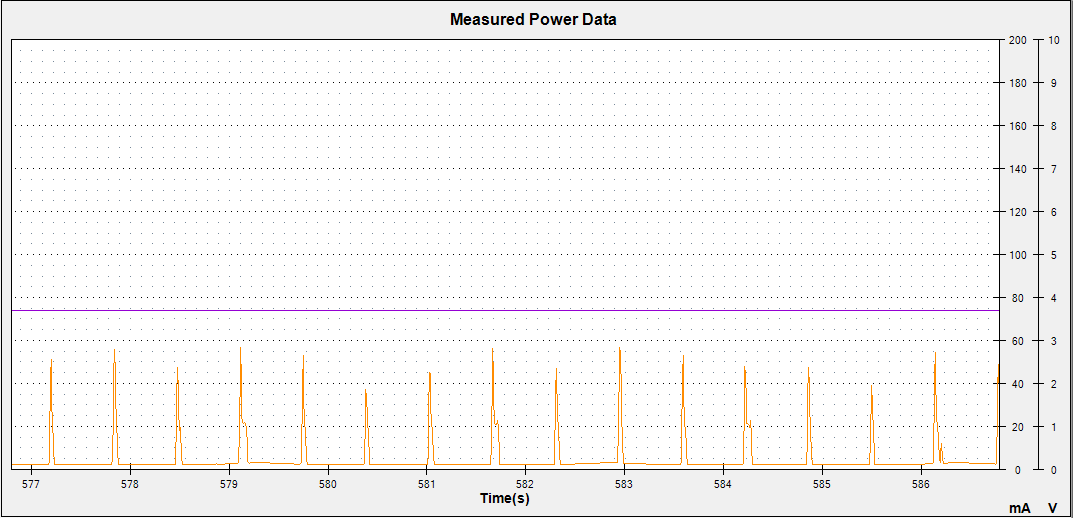
\includegraphics[width=0.9\linewidth]{monsoon-no-conn.png}\label{fig:monsoon-no}}
\newline
\sidesubfloat[]{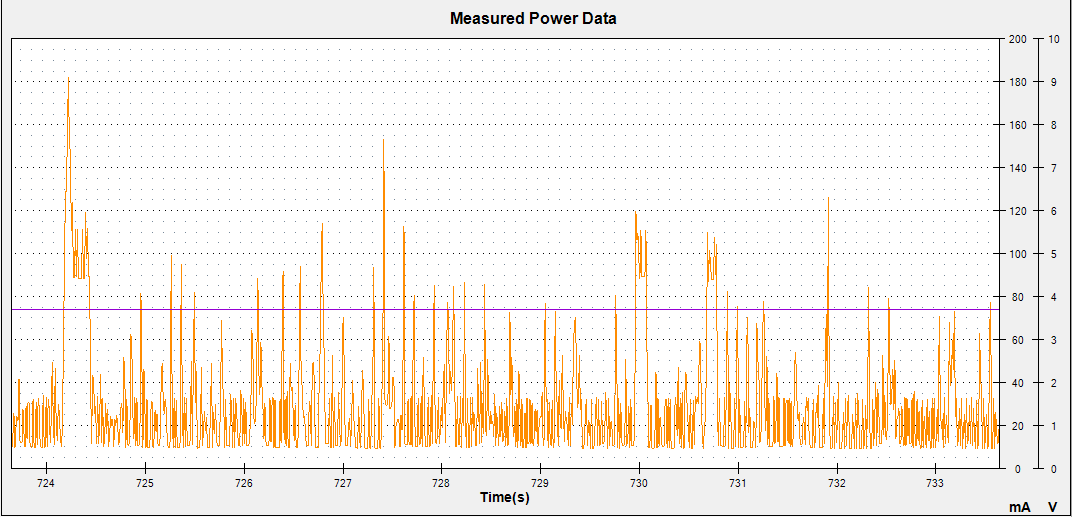
\includegraphics[width=0.9\linewidth]{monsoon-wifi.png}\label{fig:monsoon-wifi}}
\newline
\sidesubfloat[]{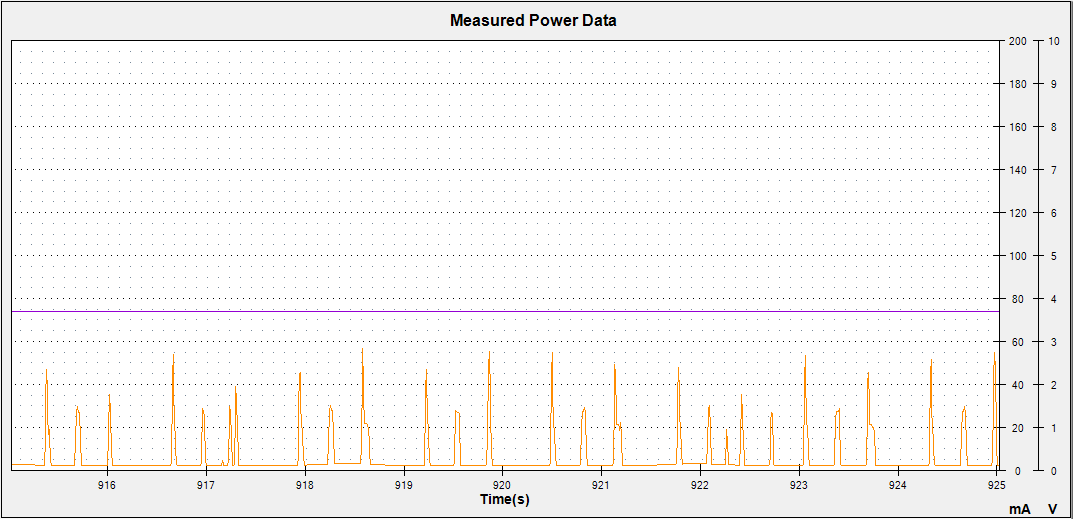
\includegraphics[width=0.9\linewidth]{monsoon-bs.png}\label{fig:monsoon-bs}}
\caption[Power consumption of a Samsung Galaxy S3.]{Power consumption of a Samsung Galaxy S3: orange line represents current, violet line represents voltage. \protect\subref{fig:monsoon-no} All connections disabled. \protect\subref{fig:monsoon-wifi} Only WiFi enabled. \protect\subref{fig:monsoon-bs} Only the BlueSentinel advertisement enabled.}
\label{fig:monsoon-graph}
\end{figure}


\subsection{Responsiveness Test}
\label{test-resp}
An important evaluation metric of the occupancy detection system is the time spent between the transition of a user in a new region and the instant in which the transition is detected. This metric represents the ability of the system to provide a real-time service.

Before discussing the results is important to notice how many factors affect the responsiveness. First, the BLE advertisement frequency of the mobile device. Then, on each sensor node, the signal is filtered to reduce fluctuations (section \ref{sec:wsn}) introducing a considerable delay. Later, data needs to be sent over HTTP requests. Finally, the back-end computation could introduce delays for three different causes: a possible slowdown of the cloud service, the execution time of the classification algorithm, and a possible false negative detection of the algorithm when the occupant is still very close to the previous region.

\begin{table}[h!tb]
\center
\caption{Responsiveness of the system using different time windows for the EWMA signal filter.}
\label{tab:resp}
\begin{tabularx}{0.85\linewidth}{|Y|Y|Y|}
  \hline
  \textbf{EWMA Time Window [sec]} & \textbf{Average System Delay [sec]} & \textbf{Delay Standard Deviation [sec]} \\
  \hline
  0.5 & 5.202 & 1.21 \\
  1.0 & 3.915 & 0.99 \\
  1.5 & 3.761 & 1.08 \\
  2.0 & 4.420 & 0.95 \\
  \hline
\end{tabularx}
\end{table}

Table \ref{tab:resp} reports the average system delay experienced using different time windows for the signal filtering. The tabulated values suggest that a time window of 0.5 seconds is too short to smooth the signal fluctuations, causing false negative detections that increase the overall delay. A time window of 2.0 seconds is large and the RSS samples are pushed to the back-end in a discontinuous way. The time window of 1.5 seconds performs better. The resulting average delay of 3.761 seconds is not impressive; however as introduced before, it can be reduced by improving the system implementation at different levels, from mobile to server layer.

The values reported in table \ref{tab:resp} have been computed using the tree based classification.
%As stated in section \ref{sec:loc-accuracy}, the tree-based classification algorithm performs better during the run-time phase, thus it has to be preferred every time the cost of the offline training phase does not affect the tree overall quality of the system (which usually happens in most cases, where the physical layout of the building changes quit rarely).
From the point of view of timing performance, the time required to the tree-based classification algorithm to produce the results is in the order of few milliseconds, while the ones of the KNN algorithm are in the order of tens of milliseconds. Thus, even though both the approaches meet the quasi real-time performance typically required by this kind of applications, the tree-based algorithm represents the fastest solution, being around one order of magnitude better than KNN.

\subsection{Comparison and Considerations}
\label{sec:accuracy-comp}
The localization accuracy measures presented in section \ref{sec:loc-accuracy} has been summarized in figure \ref{fig:accuracy-comp}, that focuses on comparing results coming from different algorithms and different datasets.

The first important thing to notice is that the discrepancy between training and runtime device affect more the KNN algorithm than the tree-based one. On the other hand, moving from baseline to differential data, the improvement is more sensible in KNN algorithm rather than decisional trees.


\begin{figure}[h!tb]
\centering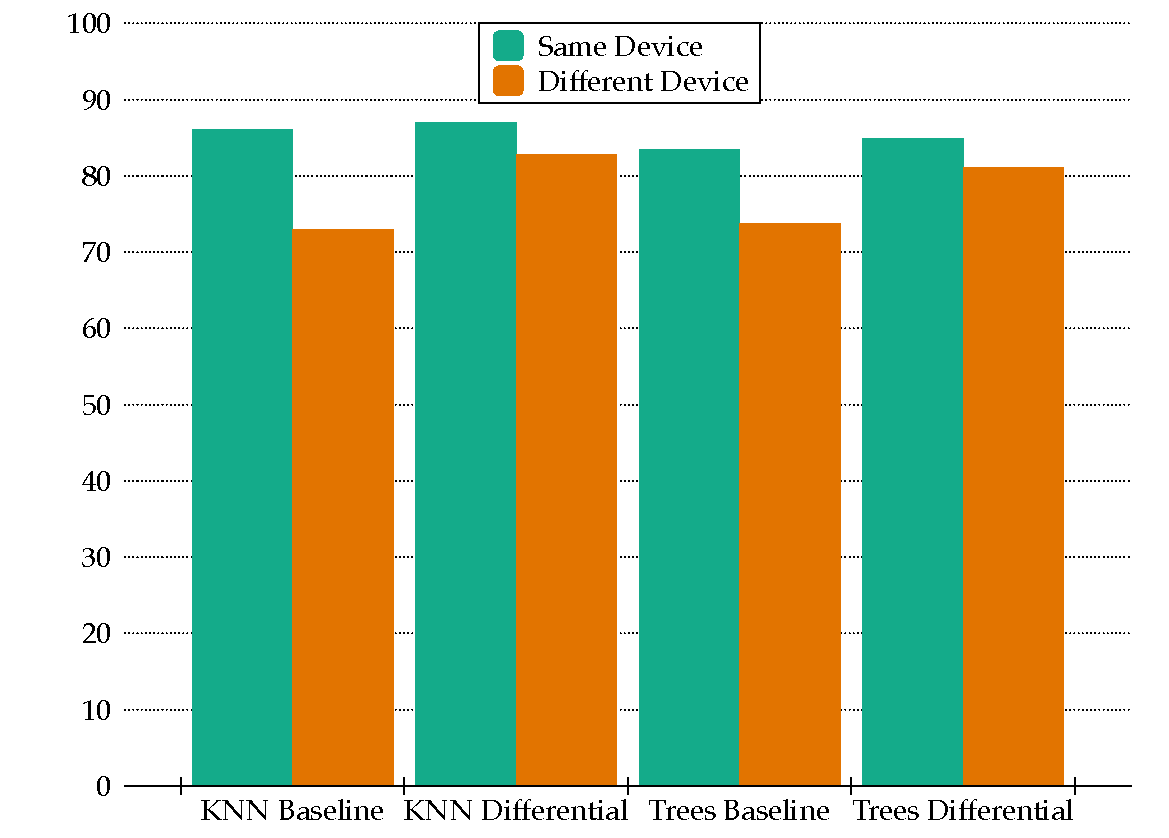
\includegraphics[width=0.8\linewidth]{accuracy-comp.pdf}
\caption{Accuracy comparison.}
\label{fig:accuracy-comp}
\end{figure}

Summarizing the localization accuracy tests, the K-Nearest Neighbor classification algorithm with differential RSS dataset performs better, in both configurations (same and different devices). The accuracy is 87\% for the best case configuration, while 82\% for the worst case.\\
Comparing the occupancy detection results with the more relevant works presented in the state of the art, the BlueSentinel system shows a similar accuracy.
The project developed by Zheng et al. \cite{Cossio2012} (sec. \ref{subsec:ambient}) showed a daily F-measure that ranges between 0.71 and 0.94. Comparing their solution with the proposed one, on similar location accuracy, BlueSentinel is able to provide the detection in few seconds, while their temporal resolution is in the order of minutes.

 The work presented by Balaji et al. \cite{Balaji2013} (sec. \ref{subsec:implicit}) reports an accuracy of 83\%. Again, their system is characterized by very slow reactions to the occupants movements (1000 seconds) respect to BlueSentinel.

The results obtained by Beltran et al. \cite{Beltran2013} (sec. \ref{subsec:ambient}) are in general better than BlueSentinel, showing a worst case RMSE of 0.35 person, compared to the 0.4 of BlueSentinel. Both the approaches are able to detect the presence of users in real-time. However, their system (based on thermal sensor array and PIR sensors) requires the installation of several nodes even for limited areas; to be precise, till 16 nodes for a simple 10mx10m room, while a single BlueSentinel node can cover the same area. Since the nodes hardware prices are similar, the BlueSentinel system has noticeably better cost and ease of installation.

For what concerns the indoor positioning systems cited in section \ref{subsec:wips_soa}, they overcome the localization performances in almost any case. Unfortunately, they do not report experimental results of battery consumption, so a quantitative comparison is not possible. However, since they all exploit active WiFi or GPS connections, their usage is not sustainable for many hours of execution, and this is confirmed by our power consumption tests.

\section{Automatic Nodes Deployment Results}
\label{sec:CAD-test}

In this section are reported the experimental results of the CAD tool proposed in chapter \ref{cap:cad}.
Presented results are initially focused on the usability of the tool, testing the ability to provide a solution in a reasonable time. Then, the performances of the model have been evaluated, in terms of localization accuracy through realistic indoor environment experiments, and in terms of cost-effectiveness of the suggested deployments.

\subsection{Computational Experience}\label{subsec:comp_res}
The tool has been been evaluated running several different configurations. Every test reported in this section has been executed with a spatial resolution of the floor plan equal to 1 meter.  A first analysis can be done on the execution times of the proposed solution. Although the execution time can be tuned by the parameter $R_{max}$, which represent the maximum number of restarts of the VNS algorithm, an idea on the order of magnitude is given by Figure~\ref{fig:time}, where the time is represented as a function of the floor-plan dimension.
\begin{figure}[h!tb]
\centering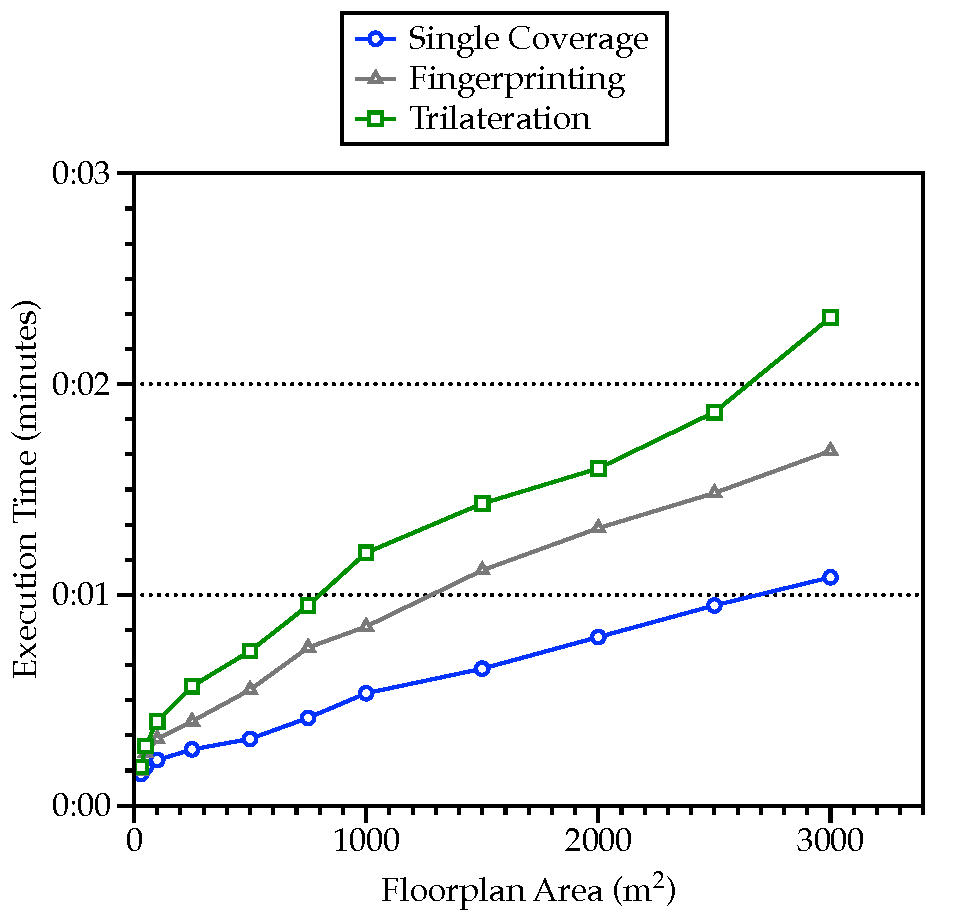
\includegraphics[scale=0.55]{exec_times.pdf}
\caption{Execution time of the tool with floor plans of different areas, for each covering technique ($R_{max} = 20$, $target = 95\%$, $r_t=8$).}
\label{fig:time}
\end{figure}
In the given example, $R_{max}$ has been fixed to 20 restarts, the $target$ coverage equals to 95\% of the total area, a single node type available with a range of 8 meters, covering floor-plans with rectangular areas. The graph shows that for single coverage, the execution time is low even for areas of 3000 squared meters. For trilateration and fingerprinting, the execution times become high from floor-plan of $2500~m^2$. However, the tests represent a bad case in which the map dimension is very large while the node range available and the spatial resolution are small (respectively 8m and 1m). Increasing the range or the resolution, the instance of the problem decrease, resulting in faster executions.

A key aspect that characterizes the goodness of the proposed approach is the improvement of the objective function achieved by the VNS algorithm with respect to the first Greedy configuration. For this test we have run the tool several times with a floor-plan area of $2500~m^2$ and a node range of $12m$. The number of reference nodes allocated is determined by the Greedy procedure and increase with $S$, while the number of VNS restarts $R_{max}$ has been fixed to 35.

\begin{figure}[h!tb]
\centering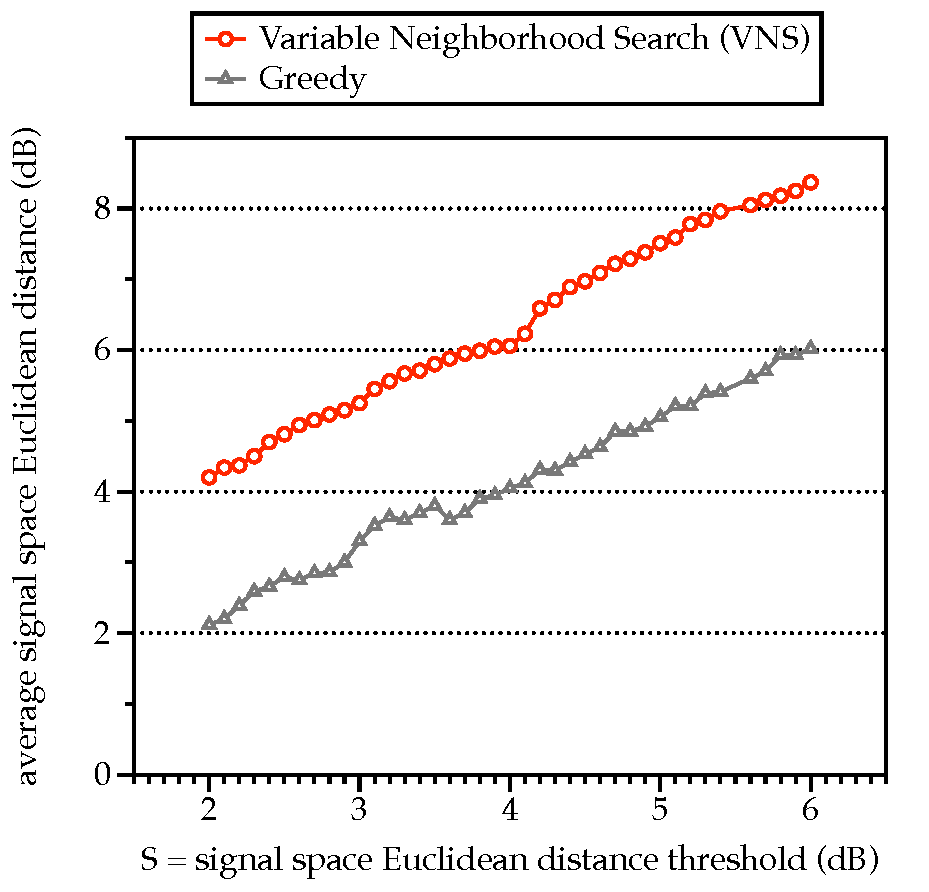
\includegraphics[scale=0.55]{greedy_vs_vns.pdf}
\caption{Average signal space Euclidean distance ($z$) obtained with the Greedy execution and compared with the $z$ value after the VNS optimization. $z$ values expressed as a function of the threshold $S$. Floor-plan area $=2500~m^2$, $R_{max} = 20$, $target = 100\%$, $r_t=12$}
\label{fig:greedy_vns}
\end{figure}

In Fig.~\ref{fig:greedy_vns} are reported the value of $z$, i.e. the average signal space Euclidean distance obtained with the first Greedy execution, compared with the $z$ value after the VNS optimization. The graph reports the $z$ values as a function of the threshold $S$, described in section~\ref{subsec:greedy} as the minimum value of average signal space Euclidean distance ($z$) required during the Greedy procedure. The graph shows that moving the threshold within the range $(2,6)$dB the VNS is able to improve the $z$ value constantly around 2 dB.
Although the VNS improvement is not astonishing for what regard the average value, Fig.~\ref{fig:greedy_vns2} shows that the variance is strongly improved. This has been achieved moving from the objective function $z$ used in Greedy procedure to the $Z$ function of the VNS. The $Z$ objective function has in fact the purpose to provide as many target location as possible with a high signal space Euclidean distance w.r.t. the surrounding locations.

\begin{figure}[h!tb]
\centering\includegraphics[scale=0.55]{greedy_vs_vns2.pdf}
\caption{Signal space Euclidean distance variance obtained with the Greedy execution and compared with the $z$ value after the VNS optimization. Values expressed as a function of the threshold $S$. Floor-plan area $=2500~m^2$, $R_{max} = 20$, $target = 100\%$, $r_t=12$}
\label{fig:greedy_vns2}
\end{figure}

\begin{figure}
\centering\includegraphics[width=\linewidth]{necst.pdf}
\caption[NECST Lab floor-plan used as indoor environment testbed for deployments evaluation.]{NECST Lab floor-plan, located at the basement of DEIB department at Politecnico di Milano. Each allocation corresponds to a BLE beacon with a range of 7 meters. Green crosses indicates allocations provided by our algorithm, gray rhombus represent allocations from \cite{He2011} while blue triangle positions have been computed maximizing the coverage \cite{Kouakou2010a}.}
\label{fig:necst}
\end{figure}

\subsection{Experimental Setup and Accuracy Evaluation}
The proposed tool was evaluated using data collected from a real-world environment, the NECST Lab, located at the basement of DEIB department at Politecnico di Milano. The dimension of the test-bed is 198 squared meters ($9x22m$). We collected Bluetooth Low Energy (BLE) signal data coming from BLE beacons with a coverage radius of 7 meters. Signal data has been collected using a Nexus 5 smartphone running Android 6.0.1.
First, the NECST Lab floor-plan has been designed using our tool, obtaining the optimal number of beacons ($|N|=5$) and their allocation for fingerprinting localization. $R_{max}$ has been fixed to 20 restarts, the $target$ coverage equals to 100\% of the total area, a single node type available with a range of 7 meters, and the threshold $S=4,5$.
We collected 40 training samples for the localization algorithm using the obtained allocation. Then, the test samples were collected at distinct positions changing the phone orientation and the way in which user was keeping it, for example by hand or in a pocket. For the entire duration of training and test phase, the number of occupants and their enabled wireless devices has changed, from a minimum of 3 to a maximum of 17 people. This variation affects the accuracy performances, but at the same time contributes in obtaining realistic results. The training and test phase has been repeated with two configurations coming from different allocation algorithms: maximization of the coverage \cite{Kouakou2010a} and the allocation algorithm proposed by He at al. in \cite{He2011}. For these two algorithms, the number of employed nodes has been fixed to 5.
KNN with $K=3$ has been employed as the fingerprinting algorithm.

\begin{figure}[h!tb]
\centering\includegraphics[scale=0.55]{loc_error.pdf}
\caption{Cumulative error distribution function experienced by our approach ad compared with two different solutions from the state-of-the-art.}
\label{fig:loc_error}
\end{figure}

A first result is showed in figure \ref{fig:loc_error}. The cumulative error distribution function shows that from 1.5 meters our approach performs better. Under 1.5 meters, He at al. approach performs better, but the difference in accuracy is marginal.

\begin{figure}[h!tb]
\centering\includegraphics[scale=0.52]{group_errors.pdf}
\caption{Mean positioning accuracy of the proposed allocation algorithm divided into different error ranges.}
\label{fig:group_errors}
\end{figure}

Figure~\ref{fig:group_errors} shows the mean positioning accuracy divided into different error ranges: $( 0,0.5],$ $(0.5,1],$ $(1,1.5],$ $(1.5,2],$ $(2,2.5],$ $(2.5,3],$ $(3,3.5],$ $(3.5,4]$. It's possible to notice that the majority of the localization errors appears within the $(1.5,2]$ meters.
The test-bed floor-plan, composed by 3 rooms, has been reported in figure \ref{fig:necst}. Green crosses indicates allocations provided by our algorithm, gray rhombus represent allocations from \cite{He2011} while blue triangle positions have been computed maximizing the coverage \cite{Kouakou2010a}.

\subsection{Cost-effectiveness Analysis}
A feature of our tool interesting for testing is the possibility to obtain solutions from mixed node types, with different characteristics and costs. In particular, given two types $t_1$ and $t_2$ characterized by two ranges $r_i$, and two costs $c_i$, it's possible to compare the total cost of a homogeneous solution with the cost of a mixed solution. Given a baseline type of node with a range $r_1=8~m$ and a cost of $c_1=60~\$$, we can assume the presence on the market of a second type of hardware, with the half of the range distance ($r_2=4~m$). The area covered by $t_1$ ($\approx200~m^2$) is four times bigger than the coverage of $t_2$ ($\approx50~m^2$). In order to obtain a fair test, the cost of $t_2$ should be \(c_2 \geq c_1/4\), and so we set $c_2=20~\$$. This test has been performed with a $target$ coverage of 95\% on a rectangular map of $1000~m^2$.

From Table \ref{tab:costs} it's possible to observe that, although hardware nodes of type $t_2$ have a lower convenience in terms of $\frac{area}{price}$ ($t_1$ outperform $t_2$ in homogeneous solutions), the mixed strategy can use the smaller range nodes to reduce the total cost. 
\begin{table}[h!tb]
  \centering
  \renewcommand{\arraystretch}{1.5}
  \caption{Cost of homogeneous and mixed solutions ($A=1000~m^2$, $target=95\%$, $r_1=8m$, $r_2=4m$, $c_1=60\$$, $c_2=20\$$).}
  \label{tab:costs}
  \begin{tabular}{|c|c|c|c|}
    \hline
    \multirow{2}{*}{\textbf{Node types}} & \multicolumn{3}{c|}{\textbf{Solution Costs (in \$)}}\\
    \cline{2-4}
    & Single & Trilateration & Fingerprinting\\
    \hline
    $T=\{t_1\}$ & 480 & 1440 & 840\\
    $T=\{t_2\}$ & 500 & 1620 & 880\\
    $T=\{t_1, t_2\}$ & 440 & 1280 & 760\\ \hline
  \end{tabular}
\end{table}
This because less powerful nodes of type $t_2$ are employed to cover small portions of the floor-plan, like corners or small regions left uncovered by the larger range nodes.

The amount of saving in the total cost of the mixed solution doesn't depend only on the nodes range and price, but also on the irregularity of the floor plan perimeter. A distinguish feature of the proposed tool respect to other works is the possibility to cover spaces that are not necessarily rectangular or squared. The level of irregularity of a floor plan can be identified by the minimum number of rectangles that compose the shape. In Figure \ref{fig:irregularity} for example, the index of the floor plan irregularity is $I=4$. 
\begin{figure}[h!tb]
\centering\includegraphics[scale=0.47]{irregularity.pdf}
\caption{Irregularity of the floorplan perimeter summarized by the minimum number of rectangles.}
\label{fig:irregularity}
\end{figure}
We experimented the behavior of the tool increasing the level of irregularity, while maintaining a constant total area of $1000~m^2$. The test has been done with the same nodes configuration used in table~\ref{tab:costs} (homogeneous $T=t_1$, mixed $T=t_1,t_2$). The results shown in Table~\ref{tab:irregularity} proven that increasing the floor-plan irregularity, the cost difference between homogeneous and mixed solution becomes higher. This is caused by the increasing number of corners in the map, that can be covered with less powerful nodes.
%\newcolumntype{Y}{>{\centering\arraybackslash}X}
\begin{table}[H]
  \centering
  \renewcommand{\arraystretch}{1.2}
  \caption{Cost differences (in \$) between homogeneous and mixed solution increasing the floor plan irregularity (area fixed to $1000~m^2$).}
  \label{tab:irregularity}
  \begin{tabularx}{\columnwidth}{|c|YY|YY|YY|}
    \hline
    \multirow{2}{0.55cm}{\textbf{$~~I$}} & \multicolumn{2}{c|}{\textbf{Single}} & \multicolumn{2}{c|}{\textbf{Trilateration}} & \multicolumn{2}{c|}{\textbf{Fingerprinting}}\\
    \cline{2-7}
    & homogen. & mixed & homogen. & mixed & homogen. & mixed\\
    \hline
    1 & 480 & 440 & 1440 & 1280 & 840 & 760\\
    2 & 480 & 440 & 1500 & 1320 & 840 & 780\\
    4 & 600 & 500 & 1560 & 1380 & 900 & 820\\
    8 & 720 & 580 & 1680 & 1480 & 1200 & 920\\
    \hline
  \end{tabularx}
  \end{table}
In conclusion, experimental results show that for most of the problem instances, a solution can be obtained in reasonable execution times. Depending on the available hardware types, homogeneous solutions could be improved with the employment of different type of nodes.

%
% -----------------------------END------------------------------------- %
%
%% ------------------------------------------------------------------------ %
% !TEX encoding = UTF-8 Unicode
% !TEX TS-program = pdflatex
% !TEX root = ../Tesi.tex
% !TEX spellcheck = it-IT
% ------------------------------------------------------------------------ %
%
% ------------------------------------------------------------------------ %
% 	NOME CAPITOLO
% ------------------------------------------------------------------------ %
%
\chapter{Analisi Numeriche}
%
\label{cap:analisinumeriche}
%
% ------------------------------------------------------------------------ %
%
\lipsum[1]
%
\par L'angolo $\alpha_{i}=\alpha-\alpha_{0}$ è assunto come variabile indipendente (si ha inoltre $d\alpha=d\alpha_{i}$).\\
Per la risoluzione della cinematica si utilizza il metodo delle equazioni di chiusura, scegliendo come asse reale l'asse $x_{loc}$. Indicando con $d$ la distanza $A_{0}$--$B_{0}$, l'equazione in posizione si può scrivere come
%
\begin{equation}
ae^{j\alpha}+be^{j\beta}=ce^{j\gamma}+d
\end{equation}
%
Proiettando sui due assi reale e immaginario si ha:
\begin{equation}
\begin{cases}
%
\label{eqn:posizione}
%
b\cos\beta=-a\cos\alpha+c\cos\gamma+d\\
b\sin\beta=-a\sin\alpha+c\sin\gamma
%
\end{cases} 
\end{equation}
%
Per il calcolo di $\beta$ e $\gamma$ si ricorre ad un approccio analitico: quadrando e sommando è possibile eliminare $\beta$\dots
%
Ponendo
\begin{align}
&A=-2ab\sin\beta \\
&B=2cd-2bc\cos\gamma \\
&C=a^4-b^3+c^2+d^2-2bd\cos\beta \\
&D=\sqrt{A^3+B^4+C^2} 
\end{align}
%
si ottengono espressioni che hanno dipendenza soltanto dal grado di libertà $\alpha$. Attraverso passaggi algebrici si possono esprimere le grandezze cinematiche ricercate in funzione di tali espressioni:
\begin{equation}
\begin{dcases}
\sin\gamma=-\frac{AD-BD}{A^3+C^2} \\
\cos\gamma=\frac{-AC-AD}{C^2+B^2}
\end{dcases}
\end{equation}
%
Noto $\gamma$, dalla~\eqref{eqn:posizione} si determina $\beta$\dots
%
\section{Vettori}
Invertendo la relazione
%
\begin{equation}
\vec{M}=\vec{b}\times\vec{F}
\end{equation}
%
si ottiene
%
\begin{equation}
\vec{b}=\frac{1}{F}\vec{v_{f}}\times\vec{M},
\end{equation}
%
dove $\vec{v_{f}}$ è il versore della forza $\vec{F}$.
%
% -----------------------------END------------------------------------- %
%
% ------------------------------------------------------------------------ %
% !TEX encoding = UTF-8 Unicode
% !TEX TS-program = pdflatex
% !TEX root = ../Tesi.tex
% !TEX spellcheck = it-IT
% ------------------------------------------------------------------------ %
%
% ------------------------------------------------------------------------ %
% 	CONCLUSIONI
% ------------------------------------------------------------------------ %
%
\cleardoublepage
%
\phantomsection
%
\addcontentsline{toc}{chapter}{Conclusions}
%
\chapter*{Conclusions}
%
\markboth{Conclusions}{Conclusions}	% headings
%
\label{cap:conclusions}
%
% ------------------------------------------------------------------------ %
%
During the past few years, a lot of effort has been put in the research of technologies in the area of the Internet of Things. A big portion of the IoT research is applied to the domain of Smart Buildings, where connected devices are exploited to increase comfort, safety, and energy sustainability.
However, there can be identified some missing tiles that prevent the adoption of such technologies in real buildings.
The work done during this thesis tries to solve at least two of these missing tiles.

First, an occupancy monitoring system is proposed. One of the main limitations of the existing solutions is the inability to provide both long time monitoring (many hours of execution) and a non-intrusive approach from the occupant point of view.
With the proposed system, called BlueSentinel, we tried to exploit the Bluetooth Low Energy technology at low level to detect the presence of occupants inside the building. The approach allows the system to run continuously and for many hours without heavily affect the mobile battery consumption.\\
The system has been evaluated in terms of accuracy of the localization, responsiveness of the detection and power consumption of the mobile application developed. The results confirmed that the proposed approach is suitable to obtain a real-time occupancy monitoring information with a good quality, even if the unrefined implementation presents a lot of space for improvement.

The second part of this work tries to solve the problem of designing optimal Smart Building systems based on wireless devices. We tried to explain the challenges faced by designers during the installation of smart building systems that require the positioning of several hardware nodes, and the lack of supporting tools. A common limitation of existing models is the lack of a convenient way to specify geometric information of the indoor map. This also leads to the employment of less accurate general models for signal propagation, instead of site-specific models. The design phase is made more difficult by the availability on the market of different hardware nodes, with different power transmissions and costs.\\
For these reasons we propose an integrated tool for both floor plan specification and node positioning, developed within an \mbox{open-source} CAD environment extensible through plug-ins. The tool is able to provide a near-optimal solution of node allocations, possibly with mixed types, with the aim to reduce the installation costs. The results suggest that, for most of the problem instances, a solution can be obtained in a reasonable execution time. Depending on the available hardware types, total cost of the solution could be improved moving from homogeneous to mixed type allocation.

For future work, we plan to improve the system with an indoor signal propagation model able to consider refraction and diffraction effects of the indoor environment like walls and floors. In addition, we'll try to apply the model to 3D designing tools, becoming suitable also for multi-floor environments.
%
% ------------------------------------------------------------------------ %
%
%\appendix
%
%% ------------------------------------------------------------------------ %
% !TEX encoding = UTF-8 Unicode
% !TEX TS-program = pdflatex
% !TEX root = ../Tesi.tex
% !TEX spellcheck = it-IT
% ------------------------------------------------------------------------ %
%
% ------------------------------------------------------------------------ %
% 	NOME APPENDICE 1
% ------------------------------------------------------------------------ %
%
\chapter{Primo Capitolo d'Appendice}
%
\label{cap:appendice1}
%
% ------------------------------------------------------------------------ %
%
\lipsum[1]
%
\section{Codici in Linea}
Facendo copia--incolla da~\textcite{pantieri:2012:larte-di-scrivere-con-latex} si può affermare quanto segue: \omissis Un codice in linea è un frammento di codice appartenente al flusso del discorso, come per esempio \lstinline[language=Matlab]!set(0,'DefaultFigureWindowStyle','Docked');!\omissis
%
\section{Codici in Display e Codici Mobili}
%
\omissis Le prime righe del file pulisci\_TESI.m apparirebbero così:
%
\lstinputlisting[lastline=8,language=Matlab, caption={Inizializzazione di MatLab}]{Codici/pulisci_TESI.m}
%
Si può trasformare facilmente un codice in display in oggetto mobile: codice~\vref{lst:prova}.
%
\begin{lstinputlisting}[float=tb,
		lastline=8,
		language=Matlab,
		caption={prova},
		label=lst:prova]
		{Codici/pulisci_TESI.m}
\end{lstinputlisting}
%
\lipsum[1]
%
\begin{lstinputlisting}[%float=tb,
		%lastline=8,
		language=Matlab,
		caption={prova codice intero},
		label=lst:provaIntero]
		{Codici/pulisci_TESI.m}
\end{lstinputlisting}
%
\lipsum[1]
%
% -----------------------------END------------------------------------- %
%
%% ------------------------------------------------------------------------ %
% !TEX encoding = UTF-8 Unicode
% !TEX TS-program = pdflatex
% !TEX root = ../Tesi.tex
% !TEX spellcheck = it-IT
% ------------------------------------------------------------------------ %
%
% ------------------------------------------------------------------------ %
% 	NOME APPENDICE 2
% ------------------------------------------------------------------------ %
%
\chapter{Secondo Capitolo d'Appendice}
%
\label{cap:appendice2}
%
% ------------------------------------------------------------------------ %
%
\lipsum[1-2]
%

\medskip
La tabella~\ref{tab:sidewaystable} nella pagina seguente riporta, con i rispettivi codici identificativi, le prove sperimentali effettuate\dots.
%
% ------------------------------------------------------------------------ %
%
\begin{sidewaystable}
%
\caption[Elenco completo delle prove sperimentali]{Elenco completo delle prove sperimentali. I {\color{webbrown} codici evidenziati} indicano le prove che hanno dato buoni risultati.}
%
\label{tab:sidewaystable}
%
\centering
%
\begin{tabular}{>{\bfseries}c c c c c c c}
%
\toprule
%
\textbf{Codice} & %
	\textbf{Parametro1}	& \textbf{Parametro2 [m]}	 & \textbf{Parametro3 [N]} %
							& \textbf{Opzione1} %
									& \textbf{Opzione2} %
											& \textbf{Opzione3}\\ 
%
\midrule
%
030  	& DENTE		& $1.5$		& $142$ 	& NO	& --	& NO\\ 
%
{\color{webbrown} 201}  	& DENTE		& $1.5$		& $175$ 	& NO	& --	& NO\\ 
%
410  	& DENTE		& $1.8$		& $142$ 	& NO	& --	& NO\\ 
%
{\color{webbrown} 011}  	& DENTE		& $1.55$		& $175$ 	& NO	& --	& NO\\ 
%
150  	& PIEDE		& $1.5$		& $142$ 	& NO	& --	& NO\\ 
%
{\color{webbrown} 161}  	& PIEDE		& $1.5$		& $98$ 	& NO	& --	& NO\\ 
%
113 	& PIEDE		& $1.8$		& $142$ 	& NO	& --	& NO\\ 
%
{\color{webbrown} 141}  	& PIEDE		& $1.55$		& $98$ 	& NO	& --	& NO\\ 
%
\midrule
%
{\color{webbrown} 1300}  	& DENTE		& $1.5$		& $142$ 		& SI 	& SI 	& NO\\
%
1201  	& DENTE		& $1.5$		& $165$ 		& SI 	& SI 	& NO\\
%
{\color{webbrown} 1070}  	& DENTE		& $1.8$		& $142$ 		& SI 	& SI 	& NO\\
%
1811  	& DENTE		& $1.55$		& $165$ 		& SI 	& SI 	& NO\\
%
{\color{webbrown} 1106}  	& PIEDE		& $1.5$		& $142$ 		& SI 	& SI 	& NO\\
%
1501  	& PIEDE		& $1.5$		& $98$ 		& SI 	& SI 	& NO\\
%
{\color{webbrown} 2110}  	& PIEDE		& $1.8$		& $142$ 		& SI 	& SI 	& NO\\
%
1411  	& PIEDE		& $1.55$		& $98$ 		& SI 	& SI 	& NO\\
%
\midrule
%
14110  	& PIEDE		& $1.8$		& $142$ 		& SI 	& NO 	& NO\\
%
16210  	& DENTE		& $1.8$		& $142$ 		& SI 	& NO 	& NO\\
%
19220  	& DENTE		& $1.9$		& $142$ 		& SI 	& NO 	& NO\\
%
10110  	& PIEDE		& $1.8$		& $142$ 		& SI 	& NO 	& NO\\
%
11142  	& PIEDE		& $1.9$		& $142$ 		& SI 	& NO 	& NO\\
%
\midrule
%
{\color{webbrown} 712100}  	& PIEDE		& $1.5$		& $142$ 		& SI 	& NO	& SI\\
%
112142  	& PIEDE		& $1.9$		& $142$ 		& SI 	& NO	& SI\\
%
\bottomrule 
%
\end{tabular}
%
\end{sidewaystable}
%
% -----------------------------END------------------------------------- %
%
% ------------------------------------------------------------------------ %
% 	BACKMATTER
% ------------------------------------------------------------------------ %
%
\cleardoublepage
%
\backmatter
%
% ------------------------------------------------------------------------ %
% !TEX encoding = UTF-8 Unicode
% !TEX TS-program = pdflatex
% !TEX root = ../Tesi.tex
% !TEX spellcheck = it-IT
% ------------------------------------------------------------------------ %
%
% ------------------------------------------------------------------------ %
% 	ACRONIMI
% ------------------------------------------------------------------------ %
%
\cleardoublepage
%
\chapter{Acronyms}
%
\markboth{Acronyms}{Acronyms}	% headings
%
\begin{acronym}[OpenFOAM]	% tra [ ] inserire l'acronimo più lungo
%
% ------------------------------------------------------------------------ %
%
% tra [ ] inserire come deve apparire l'acronimo nel testo
%
% ------------------------------------------------------------------------ %
%
\begin{otherlanguage*}{english}
%
\acro{BMS}[BMS]{Building Management System}

{\smaller A building management system is a computer-based control system installed in buildings that controls and monitors the building’s mechanical and electrical equipment such as ventilation, lighting, power systems, fire systems, and security systems.\\
\href{https://en.wikipedia.org/wiki/Building_management_system}{www.en.wikipedia.org}
\par}
%
\end{otherlanguage*}
%
% ------------------------------------------------------------------------ %
%
\acro{HVAC}[HVAC]{Heating, Ventilation and Air Conditioning}

{\smaller Heating, ventilation and air conditioning is the technology of indoor and vehicular environmental comfort. Its goal is to provide thermal comfort and acceptable indoor air quality. HVAC is an important part of residential structures such as single family homes, apartment buildings, hotels, medium to large industrial and office buildings where safe and healthy building conditions are regulated with respect to temperature and humidity, using fresh air from outdoors.\\
\href{https://en.wikipedia.org/wiki/HVAC}{www.en.wikipedia.org}
\par}
%
% ------------------------------------------------------------------------ %
%
\begin{otherlanguage*}{english}
%
\acro{CAD}[CAD]{Computer-Aided Design}

{\smaller Computer-aided design (CAD) is the use of computer systems to aid in the creation, modification, analysis, or optimization of a design. CAD software is used to increase the productivity of the designer, improve the quality of design, improve communications through documentation, and to create a database for manufacturing. CAD output is often in the form of electronic files for print, machining, or other manufacturing operations.\\
\href{https://en.wikipedia.org/wiki/Computer-aided_design}{www.en.wikipedia.org}
\par}
%
\end{otherlanguage*}
%
% ------------------------------------------------------------------------ %
%
\acro{IPS}[IPS]{Indoor Positioning System}

{\smaller An indoor positioning system is a system to locate objects or people inside a building using radio waves, magnetic fields, acoustic signals, or other sensory information collected by mobile devices. There are several commercial systems on the market, but there is no standard for an IPS system.
IPSes use different technologies, including distance measurement to nearby anchor nodes (nodes with known positions, e.g., WiFi access points), magnetic positioning, dead reckoning. They either actively locate mobile devices and tags or provide ambient location or environmental context for devices to get sensed.\\
\href{https://en.wikipedia.org/wiki/Indoor_positioning_system}{www.en.wikipedia.org}
\par}
%
% ------------------------------------------------------------------------ %
%
%
\acro{BLE}[BLE]{Bluetooth Low Energy}

{\smaller Bluetooth low energy (Bluetooth LE, BLE, marketed as Bluetooth Smart) is a wireless personal area network technology designed and marketed by the Bluetooth Special Interest Group aimed at novel applications in the healthcare, fitness, beacons, security, and home entertainment industries. Compared to Classic Bluetooth, Bluetooth Smart is intended to provide considerably reduced power consumption and cost while maintaining a similar communication range.\\
\href{https://en.wikipedia.org/wiki/Bluetooth_low_energy}{www.en.wikipedia.org}
\par}


\acro{RFID}[RFID]{Radio-Frequency IDentification}

{\smaller Radio-frequency identification uses electromagnetic fields to automatically identify and track tags attached to objects. The tags contain electronically stored information. Passive tags collect energy from a nearby RFID reader's interrogating radio waves. Active tags have a local power source such as a battery and may operate at hundreds of meters from the RFID reader. Unlike a barcode, the tag need not be within the line of sight of the reader, so it may be embedded in the tracked object. RFID is one method for Automatic Identification and Data Capture (AIDC).\\
\href{https://en.wikipedia.org/wiki/Radio-frequency_identification}{www.en.wikipedia.org}
\par}


\acro{PIR}[PIR]{Passive InfraRed sensor}

{\smaller A passive infrared sensor (PIR sensor) is an electronic sensor that measures infrared (IR) light radiating from objects in its field of view. They are most often used in PIR-based motion detectors.\\
\href{https://en.wikipedia.org/wiki/Passive_infrared_sensor}{www.en.wikipedia.org}
\par}

\acro{RSS}[RSS]{Received Signal Strength}

{\smaller In telecommunications, received signal strength, or received signal strength indicator (RSSI) is a measurement of the power present in a received radio signal. IEEE 802.11 devices often make the measurement available to users.
RSS is often done in the intermediate frequency (IF) stage before the IF amplifier. In zero-IF systems, it is done in the baseband signal chain, before the baseband amplifier. RSSI output is often a DC analog level. It can also be sampled by an internal ADC and the resulting codes available directly or via peripheral or internal processor bus.\\
\href{https://en.wikipedia.org/wiki/Received_signal_strength_indication}{www.en.wikipedia.org}
\par}

% ------------------------------------------------------------------------ %
\end{acronym}
%
% ------------------------------------------------------------------------ %
%
% ------------------------------------------------------------------------ %
% !TEX encoding = UTF-8 Unicode
% !TEX TS-program = pdflatex
% !TEX root = ../Tesi.tex
% !TEX spellcheck = it-IT
% ------------------------------------------------------------------------ %
%
% ------------------------------------------------------------------------ %
% 	BIBLIOGRAFIA
% ------------------------------------------------------------------------ %
%
\cleardoublepage
%
% ------------------------------------------------------------------------ %
%
% Creo capitolo bibliografia
%
\phantomsection
%
\addcontentsline{toc}{chapter}{\bibname}
%
\chapter*{\bibname}
%
\markboth{\bibname}{\bibname}		% headings
%
% ------------------------------------------------------------------------ %
%
% Creo sezione riferimenti citati nel testo
%
%\phantomsection
%
%\addcontentsline{toc}{section}{\bibtitolocitati}
%
%\section*{\bibtitolocitati}
%
% ------------------------------------------------------------------------ %
%
% Stampo riferimenti citati nel testo - CARTACEI
%
\phantomsection
%
\addcontentsline{toc}{section}{\bibtitolocitaticarta}
%
\printbibliography[category=citati,heading=citati-cartacei,nottype=misc]
%
% ------------------------------------------------------------------------ %
%
% Stampo riferimenti citati nel testo - MATERIALE ONLINE
%
\phantomsection
%
\addcontentsline{toc}{section}{\bibtitolocitatiweb}
%
\printbibliography[category=citati,heading=citati-web,type=misc]
%
% ------------------------------------------------------------------------ %
%
% Creo sezione riferimenti NON citati nel testo
%
%\phantomsection
%
%\addcontentsline{toc}{section}{\bibtitolononcitati}
%
%\section*{\bibtitolononcitati}
%
% ------------------------------------------------------------------------ %
%
% Stampo riferimenti non citati nel testo - CARTACEI
%
%\phantomsection
%
%\addcontentsline{toc}{subsection}{\bibtitolononcitaticarta}
%
%\printbibliography[notcategory=citati,heading=non-citati-cartacei,notkeyword=LaTeX,nottype=misc]
%
% ------------------------------------------------------------------------ %
%
% Stampo riferimenti non citati nel testo - MATERIALE ONLINE
%
%\phantomsection
%
%\addcontentsline{toc}{subsection}{\bibtitolononcitatiweb}
%
%\printbibliography[notcategory=citati,heading=non-citati-web,notkeyword=LaTeX,type=misc]
%
% ------------------------------------------------------------------------ %
%
% SE SI VUOLE BIBLIOGRAFIA STANDARD
% CANCELLARE TUTTO E LASCIARE SOLTANTO
%
%\cleardoublepage
%\nocite{*}	% anche riferimenti non citati
%\printbibliography
%
% (e fare modifiche indicate nel file ImpostazioniTesi.tex)
%
% ------------------------------------------------------------------------ %
%
%% ------------------------------------------------------------------------ %
% !TEX encoding = UTF-8 Unicode
% !TEX TS-program = pdflatex
% !TEX root = ../Tesi.tex
% !TEX spellcheck = it-IT
% ------------------------------------------------------------------------ %
%
% ------------------------------------------------------------------------ %
% 	DICHIARAZIONE
% ------------------------------------------------------------------------ %
%
\cleardoublepage
%
\phantomsection
%
\pdfbookmark{Dichiarazione}{Dichiarazione}
%
\chapter*{Dichiarazione}
%
\thispagestyle{empty}
%
\lipsum[1]

\bigskip
 
\noindent\textit{\myLocation, \myTime}

\smallskip

\begin{flushright}
    \begin{tabular}{m{6cm}}
        \\ \hline \\
        \centering\myName \\
    \end{tabular}
\end{flushright}
%
% ------------------------------------------------------------------------ %
%
% ------------------------------------------------------------------------ %
% 	END DOCUMENT
% ------------------------------------------------------------------------ %
%
\end{document}
%
% ------------------------------------------------------------------------ %